%% 
%% Copyright 2007-2019 Elsevier Ltd
%% 
%% This file is part of the 'Elsarticle Bundle'.
%% ---------------------------------------------
%% 
%% It may be distributed under the conditions of the LaTeX Project Public
%% License, either version 1.2 of this license or (at your option) any
%% later version.  The latest version of this license is in
%%    http://www.latex-project.org/lppl.txt
%% and version 1.2 or later is part of all distributions of LaTeX
%% version 1999/12/01 or later.
%% 
%% The list of all files belonging to the 'Elsarticle Bundle' is
%% given in the file `manifest.txt'.
%% 

%% Template article for Elsevier's document class `elsarticle'
%% with numbered style bibliographic references
%% SP 2008/03/01
%%
%% 
%%
%% $Id: elsarticle-template-num.tex 168 2019-02-25 07:15:41Z apu.v $
%%
%%
\documentclass[preprint,12pt]{elsarticle}
\usepackage{xcolor}
\pagecolor{white}
\usepackage{hyperref}
\usepackage{subcaption}
%% Use the option review to obtain double line spacing
%% \documentclass[authoryear,preprint,review,12pt]{elsarticle}

%% Use the options 1p,twocolumn; 3p; 3p,twocolumn; 5p; or 5p,twocolumn
%% for a journal layout:
%% \documentclass[final,1p,times]{elsarticle}
%% \documentclass[final,1p,times,twocolumn]{elsarticle}
%% \documentclass[final,3p,times]{elsarticle}
%% \documentclass[final,3p,times,twocolumn]{elsarticle}
%% \documentclass[final,5p,times]{elsarticle}
%% \documentclass[final,5p,times,twocolumn]{elsarticle}

%% For including figures, graphicx.sty has been loaded in
%% elsarticle.cls. If you prefer to use the old commands
%% please give \usepackage{epsfig}
\usepackage{wrapfig}
\usepackage[section]{placeins}
\graphicspath{{figures/}}
%% The amssymb package provides various useful mathematical symbols
\usepackage{amssymb}
%% The amsthm package provides extended theorem environments
\usepackage{amsthm}
\usepackage{amsmath}

%% The lineno packages adds line numbers. Start line numbering with
%% \begin{linenumbers}, end it with \end{linenumbers}. Or switch it on
%% for the whole article with \linenumbers.
\usepackage{lineno}

\journal{Nuclear Physics A}

\begin{document}
%\linenumbers
\begin{frontmatter}

%% Title, authors and addresses

%% use the tnoteref command within \title for footnotes;
%% use the tnotetext command for theassociated footnote;
%% use the fnref command within \author or \address for footnotes;
%% use the fntext command for theassociated footnote;
%% use the corref command within \author for corresponding author footnotes;
%% use the cortext command for theassociated footnote;
%% use the ead command for the email address,
%% and the form \ead[url] for the home page:
%% \title{Title\tnoteref{label1}}
%% \tnotetext[label1]{}
%% \author{Name\corref{cor1}\fnref{label2}}
%% \ead{email address}
%% \ead[url]{home page}
%% \fntext[label2]{}
%% \cortext[cor1]{}
%% \address{Address\fnref{label3}}
%% \fntext[label3]{}

\title{Precision M\o ller  Polarimetry in Hall A at Jefferson Lab}

%% use optional labels to link authors explicitly to addresses:
%% \author[label1,label2]{}
%% \address[label1]{}
%% \address[label2]{}

\author[1]{J. Napolitano\corref{cor1}}
\ead{napolj@temple.edu}
\author[1]{D. C. Jones}
%\ead{donald.jones@temple.edu}
\address[1]{Temple University, Philadelphia, PA, 19122}
\author[2]{W. Henry}
\author[2]{D. G. Gaskell}
\address[2]{Jefferson Lab, Newport News, VA 23606}
\author[3]{D. E. King}
\author[3]{P. Souder}
\address[3]{Syracuse University, Syracuse, NY 13244}
\author[4]{K. Paschke}
\address[4]{University of Virginia, Charlottesville, VA 22903}
\author[5]{S. Park}
\author[5]{F. A. Gonzalez}
\author[5]{A. Deshpande}
\address[5]{Stony Brook University, Stony Brook, NY 11794}
\cortext[cor1]{corresponding author}


%\address[2]{Temple University, Philadelphia, PA, 19122}
\begin{abstract}
%% Text of abstract
The M\o ller polarimeter in Hall A at Jefferson Lab in Newport News, VA, has provided reliable measurements of electron beam polarization for the past two decades. Past experiments have typically required polarimetry at the $\gtrsim$1\% level of absolute uncertainty which the M\o ller polarimeter has delivered. However, the upcoming proposed experimental program including MOLLER and SoLID have stringent requirements on beam polarimetry at the level of 0.4\%\cite{MOLLER2014, SoLID2019}, requiring a systematic rethinking of all the contributing uncertainties. 

M\o ller polarimetry utilizes the double polarized scattering asymmetry of a polarized electron beam on a target with polarized atomic electrons. The target is a ferromagnetic material magnetized to align the spins in a given direction. In Hall A, the target is a pure iron foil aligned perpendicular to the beam and magnetized out of plane parallel or antiparallel to the beam direction. The acceptance of the detector is engineered to collect scattered electrons close to 90$^{\circ}$ in the center of mass frame where analyzing power is greatest.  The analyzing power is a function of center of mass angle, making an accurate simulation of the polarimeter acceptance critical. Complicating the simulated acceptance calculation  is the ``Levchuk'' effect discovered by Levchuk in 1992 \cite{Levchuk1992} where the intrinsic kinetic energy of the target electrons is not negligible, altering the scattering angle and thus the acceptance. Since the unpolarized inner orbital electrons have more kinetic energy than the outer polarized ones,  the acceptance change is polarization dependent.

Careful consideration has shown the two leading systematic errors come from determination of the analyzing power from simulation and from calculation of the target foil polarization.  In this paper we will discuss the main systematic errors for M\o ller polarimetry in Hall A that will have to be reduced in order to reach the goals for MOLLER and SoLID. Key to understanding has been recent insights provided by experience during the PREX-II and CREX experiments. We will discuss these insights and also revisit past calculations/assumptions that have been utilized in an effort to ensure nothing has been overlooked. 
\end{abstract}

%%Graphical abstract
%\begin{graphicalabstract}
%\includegraphics{grabs}
%\end{graphicalabstract}

%%Research highlights
\begin{highlights}
\item Research highlight 1
\item Research highlight 2
\end{highlights}

\begin{keyword}
%% keywords here, in the form: keyword \sep keyword

%% PACS codes here, in the form: \PACS code \sep code

%% MSC codes here, in the form: \MSC code \sep code
%% or \MSC[2008] code \sep code (2000 is the default)

\end{keyword}

\end{frontmatter}

%% \linenumbers

%% main text
\section{Introduction to M\o ller polarimetry}
As its name denotes, M\o ller polarimetery utilizes the analyzing power of polarized electron-electron scattering to determine the polarization of an electron beam. The polarized target is usually composed of iron or a highly ferromagnetic material. Elastically scattered events (beam electrons from atomic electrons) produce back-to-back electrons in the center of mass frame which if both detected in coincidence can be used to reduce backgrounds.

Following the analysis in \cite{Swartz1995}, M\o ller (electron-electron) scattering at tree level in the center of mass (CM) system is given by
\begin{align}
\frac{d\sigma}{d\Omega_{cm}}=&\frac{\alpha^2}{s}\frac{\left(3+\cos^2\theta\right)^2}{\sin^4\theta}\bigg[1- \bigg. \nonumber \\
&\bigg. P^{targ}_{\ell}P^{beam}_{\ell}A_{\ell}(\theta)-P^{targ}_tP^{beam}_tA_t(\theta)\cos\left(2\phi-\phi_{beam}-\phi_{targ}\right)\bigg]
\label{eq:moller_cx}
\end{align}
where the subscripts $T$ and $L$ refer to transverse and longitudinal polarization respectively. In the center of mass at high energy, the Mendalstam variable $s$ is equal to $(2E_{CM})^2$. The CM scattering angle is $\theta$ and the azimuthal angle of the target (beam) polarization with respect to the electron beam is $\phi_{targ(beam)}$. The analyzing powers for longitudinal and transverse polarization are given by
\begin{equation}
A_{\ell}(\theta)=\frac{\left(7+\cos^2\theta\right)\sin^2\theta}{\left(3+\cos^2\theta\right)^2}~~~\textrm{and}~~~A_t(\theta)=\frac{\sin^4\theta}{\left(3+\cos^2\theta\right)^2}.
\label{eq:analyzing_pow}
\end{equation}
$A_{\ell}$ is much larger than $A_t$ giving M\o ller polarimetery much more sensitivity to longitudinal polarization. Since $A_{\ell}$ is a maximum for 90 degree CM scattering where $A_{\ell}=7/9$, the optics of the M\o ller polarimeter in Hall A are tuned to accept events near this maximum. The M\o ller polarimeter in Hall A with its Fe foil polarized ``out of plane" in the beam direction ($P^{targ}_t=0$) is designed to measure the longitudinal polarization and be insensitive to the transverse polarization. Nevertheless, if the foil or magnetizing coils are not properly aligned and a transverse polarization develops, a non-negligible component of transverse asymmetry could in principle arise. In the ensuing discussion it will be assumed that the foil is properly aligned such that $P^{targ}_t=0$ and this term will be neglected. 

Integrating the cross section over the acceptance of the detector gives 
\[
\sigma \propto1-P^{targ}_{\ell}P^{beam}_{\ell}A_{zz},
\]
where $A_{zz}=\langle A_l(\theta)\rangle$, the acceptance-weighted analyzing power. We can now see that the left-right scattering asymmetry $A_{LR}$ is then given by 
\begin{equation}
A_{LR}=\frac{\sigma_R-\sigma_L}{\sigma_R+\sigma_L}=P^{targ}_{\ell}P^{beam}_{\ell}A_{zz},
\label{eq:A_LR}
\end{equation}
where $\sigma_{L(R)}$ are the cross sections for left (right) helicity electrons.

If $A_{zz}$ and the target polarization $P_{\ell}^{targ}$ are known, the beam polarization can be determined from the measured scattering asymmetry. 

In the approximation where the target electrons are at rest and the beam energy is large compared to the electron rest mass, $m_e$, there relationship between the lab momentum of the scattered electron, $p^{\prime}$, and the center of mass scattering angle is given by 
\begin{equation}
p^{\prime}=\frac{p_b}{2}\left(1+\cos\theta \right),
\label{eq:pvstheta}
\end{equation}
where $p_b$ is the electron beam momentum. Thus momentum analyzing the M\o ller scattered electrons also analyzes in $\theta$. Single arm M\o ller polarimeters leverage this characteristic to reduce potentially overwhelming Mott backgrounds. Using a narrow aperture in $\phi$ to select the scattering plane and a dipole to momentum analyze the scattering events perpendicular to the scattering plane produces a characteristic M\o ller``stripe" downstream of the dipole. In the absence of other focusing optics, the typical quadratic curvature of this stripe is a direct result of  the relationship in Eq. \ref{eq:pvstheta} which in the small angle approximation is second order in $\theta$. 


\subsection{Hall A M\o ller polarimeter design}
The polarimeter in Hall A is designed to take advantage of both the dipole momentum selection and the coincidence of dual arm detection to further reduce backgrounds. A simple schematic of the Hall A polarimeter is shown in Fig. \ref{fig:moller_diag} illustrating the key features. This polarimeter design adds to the essential elements 4 quadrupoles and an additional horizontal constraint due to the narrow apertures through the dipole. The quadrupoles are used to focus a distribution of M\o ller pairs roughly symmetric about the 90 degree center of mass through the dipole onto the detector. The additional focusing of the quadrupoles inverts the expected typical curvature of the M\o ller stripe on the detector plane as illustrated in Fig. \ref{fig:moller_diag}.
\begin{figure}[ht]
\centering
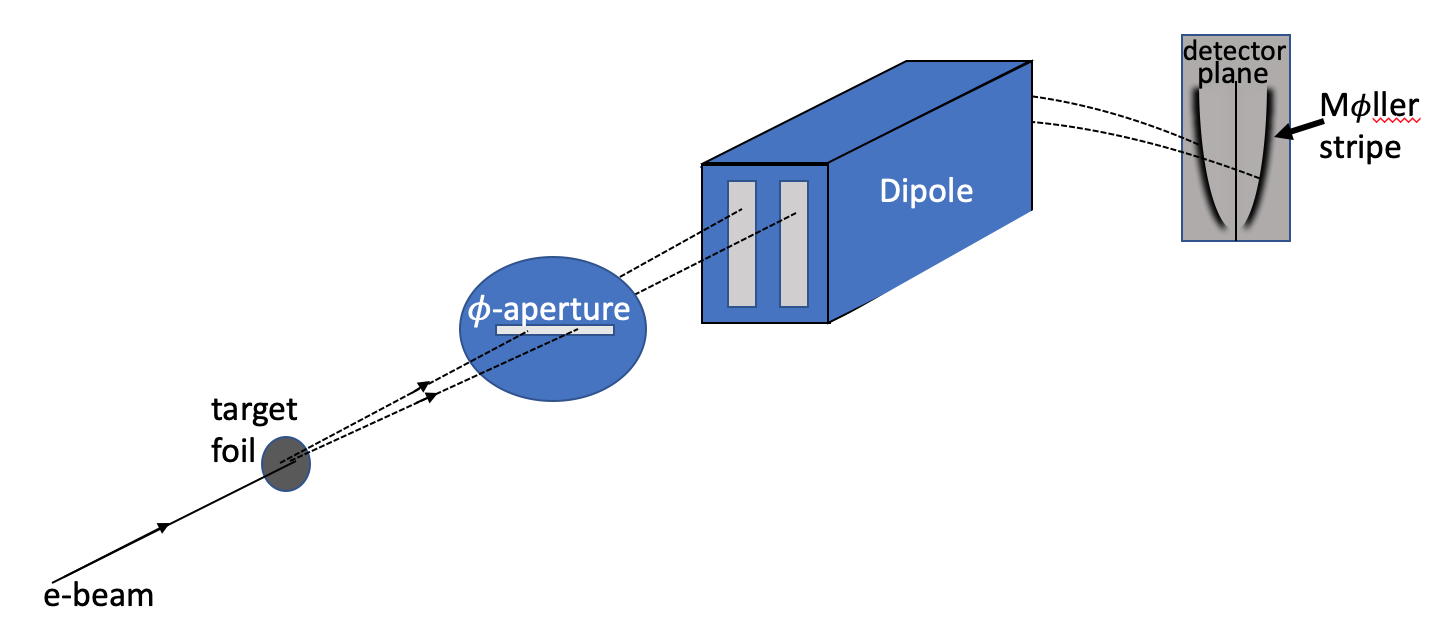
\includegraphics[width=0.7\textwidth]{simple_moller_diagram.png}
\caption{\label{fig:moller_diag}Simplified schematic showing the key features of the M\o ller polarimeter setup in Hall A. The electron beam scatters from a polarized foil target. Quadrupoles then focus the events of interest through the dipole. An aperture at the front of the dipole limits the $\phi$-acceptance defining a horizontal scattering plane. Two left-right symmetric narrow slits in the dipole momentum analyze the scattered electron pairs bending them down onto the detector plane producing characteristic M\o ller stripes.}
\end{figure}

The key elements of the M\o ller polarimeter in order going down the beamline are as follows:
\begin{enumerate}
\item{Target and its motion mechanism.}
\item{Super-conducting Helmholtz coils used to polarize the target foils.}
\item{Four quadrupoles used to focus the events of interest through the dipole.}
\item{$\phi$-acceptance defining collimator.}
\item{Dipole plus horizontal apertures.}
\item{Detector.}
\end{enumerate}
A schematic of the device including dimensions is shown in Fig. \ref{fig:G3diag}. We will briefly describe each element and the current knowledge of it. 
\begin{figure}[ht]
\centering
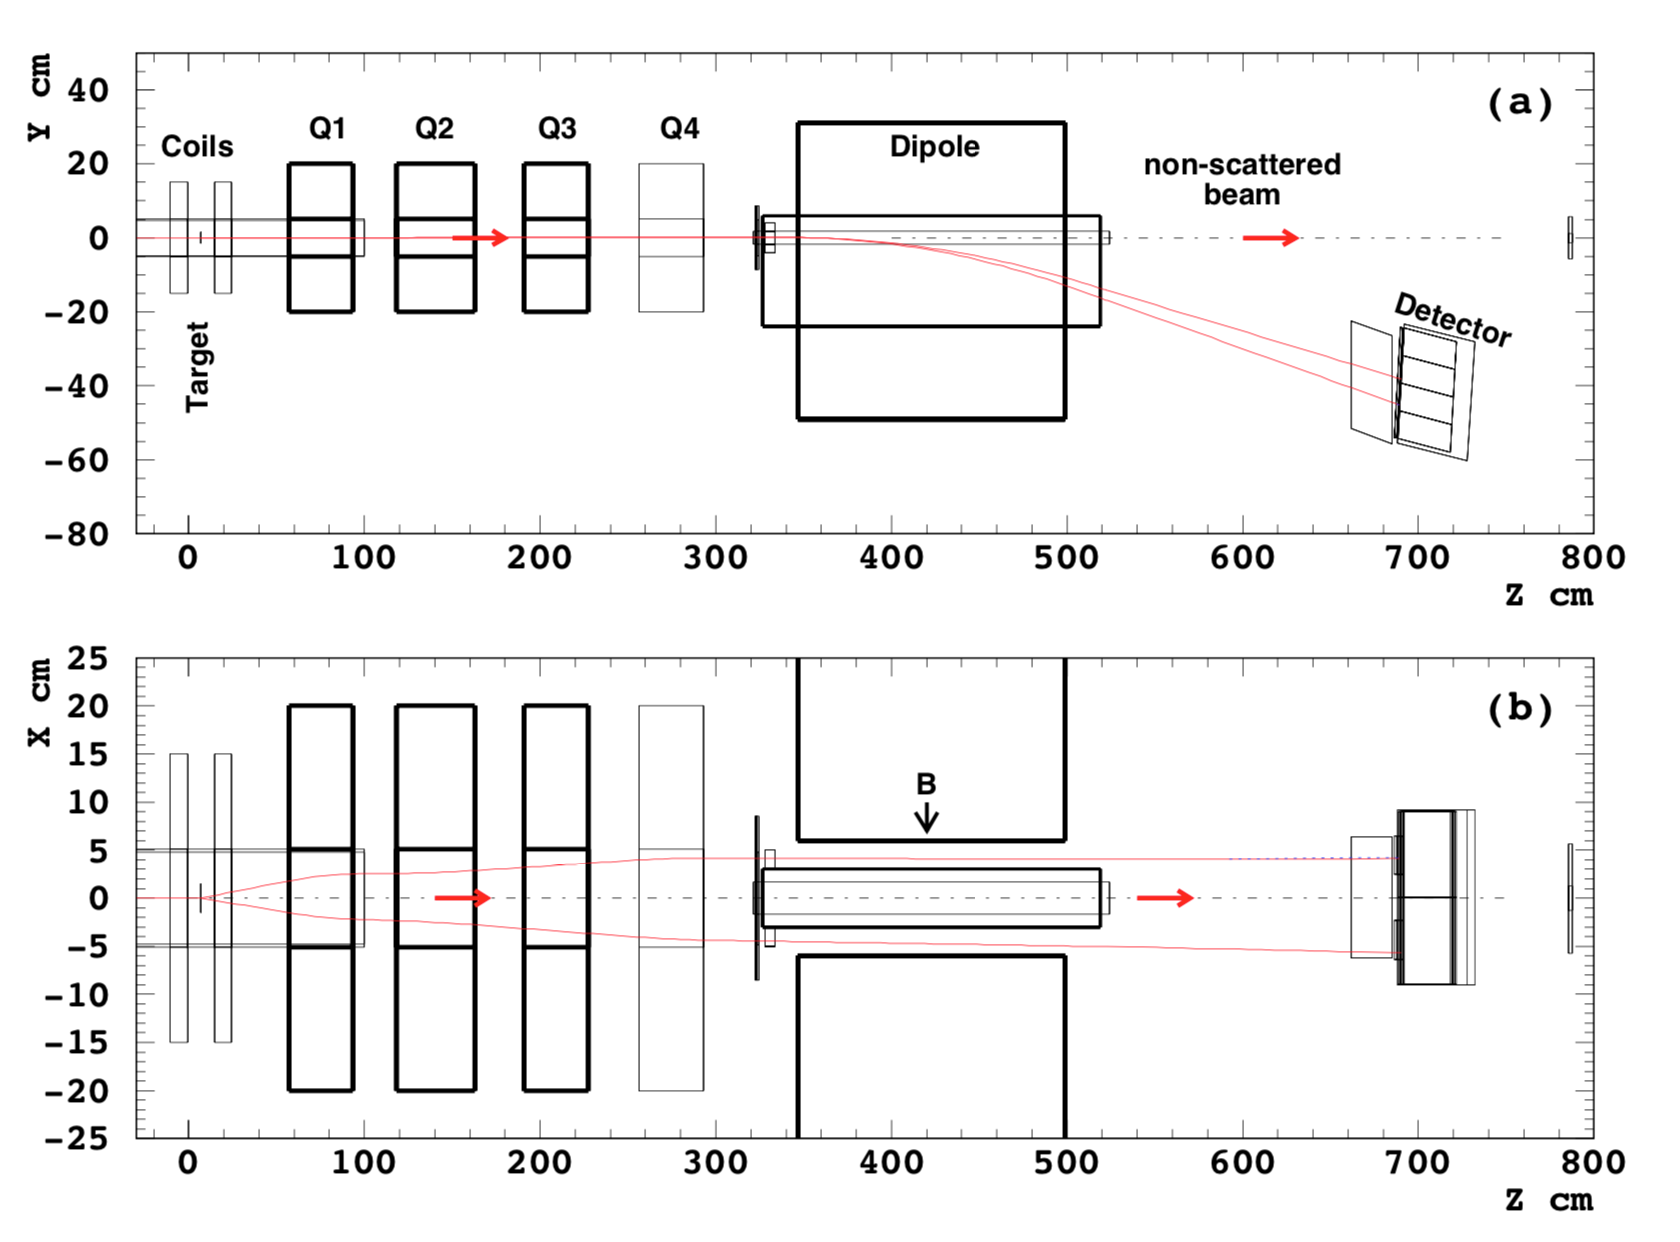
\includegraphics[width=0.9\textwidth]{G3diagram.png}
\caption{\label{fig:moller_diag}Simple schematic of the Hall A M\o ller polarimeter with dimensions.}
\end{figure}
\subsubsection{Target }
The target motion system was designed and built by Temple University. It allows for vertical insertion/extraction of the foil ladder and rotation of the foil ladder about the vertical to allow one to remove sensitivity to foil angle alignment relative to the holding field. The rotation is driven by a stepping motor attached to a 50:1 gearbox. A small bar is attached to the rotation axis to which is attached a wire potentiometer providing a voltage proportional to rotation. In principle the range of rotation can be a full 2$\pi$, however, the rod+potentiometer limits the rotation to $\pm$7 degrees. The rod motion is software limited but the rod is designed to sheer if the limits are exceeded before the system is damaged. 

\begin{figure}
\centering
\begin{tabular}{cc}
\begin{subfigure}{0.5\textwidth}
\centering
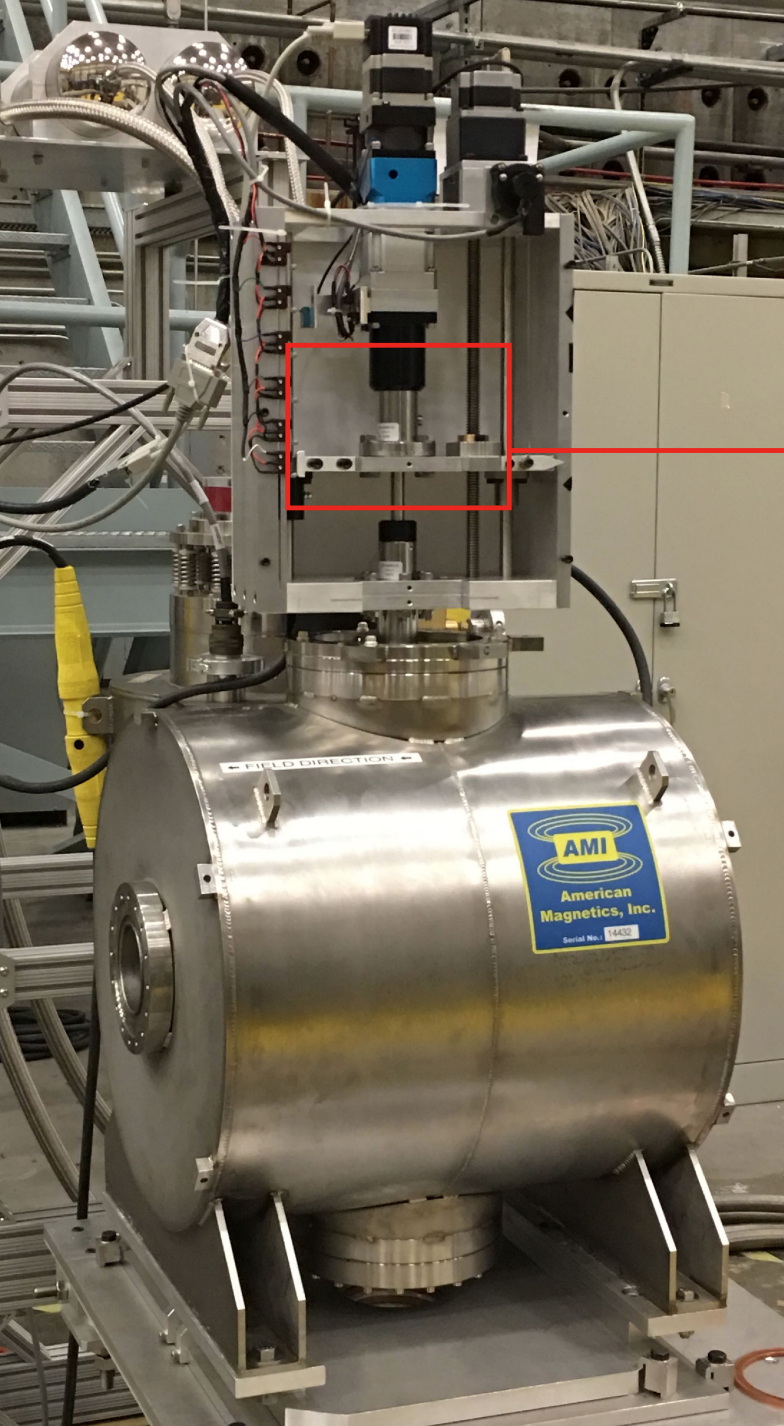
\includegraphics[width=\textwidth]{target_motion.png}
\caption{\label{fig:tgt_motion}Target motion system.}
\end{subfigure}
&
\begin{tabular}{c}
\begin{subfigure}{0.43\textwidth}
\centering
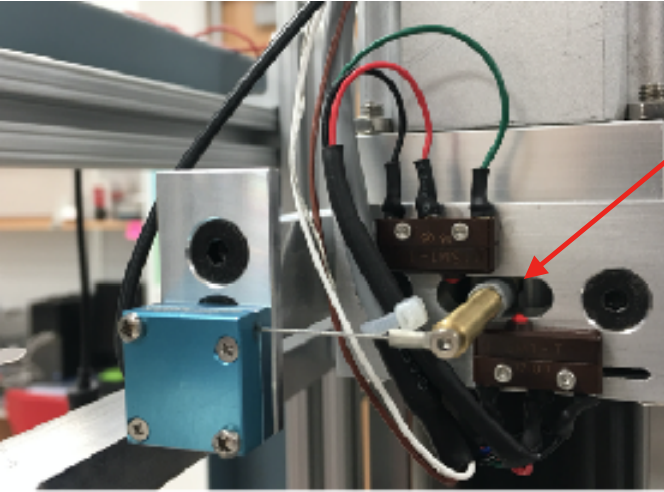
\includegraphics[width=\textwidth]{rotation.png}
\caption{\label{fig:tgt_rotation}Rotation sensor}
\end{subfigure}
\\
~\\
\begin{subfigure}{0.43\textwidth}
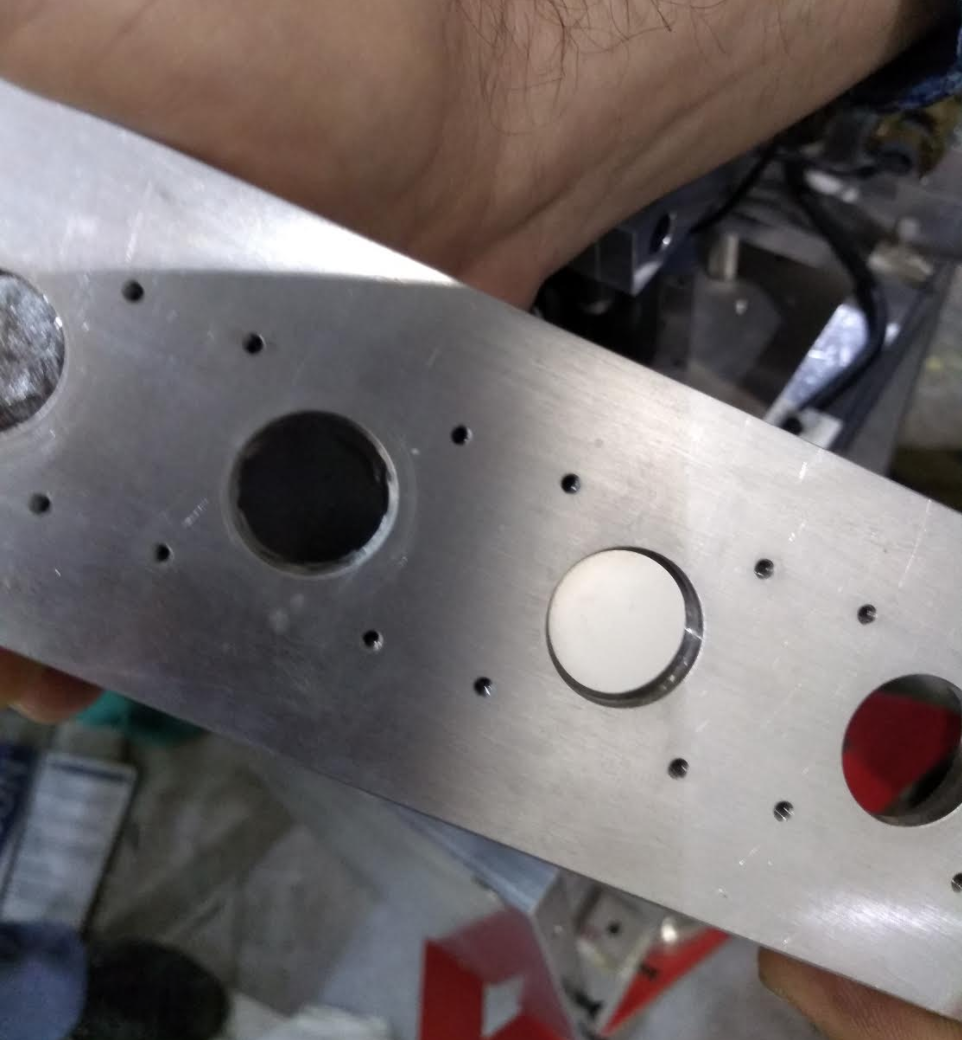
\includegraphics[width=\textwidth]{foils.png}
\caption{\label{fig:tgt_ladder}Target foil ladder.}
\end{subfigure}
\end{tabular}
\end{tabular}
\begin{center}
\caption{(a)Target motion system including vertical and rotational degrees of control. Rotation is only around the vertical. (b) Rotation measurement sensor using a brass shear rod plus a sting potentiometer. (c). Target ladder with 4 foils. From lower edge going up the foils are 11~$\mu$m Cu, 10~$\mu$m Fe,4~$\mu$m Fe, and 1~$\mu$m Fe.}
\end{center}
\end{figure}
The target ladder is designed to hold 4 thin metal foils of approximately 1 cm diameter as seen in Fig. 3c. Three Fe foils ranging in thickness from 1 ?m to 10 ?m and a single 11 ?m Cu foil are currently installed.
\subsubsection{Superconducting Helmholtz target coils}
The superconducting Helmholtz coil device used to magnetize the target foils was built by American Magnetics Inc. The system (see Fig. \ref{fig:tgt_motion}) is designed to be cryogen free in that it requires no external source of cryogenic cooling. The field at the center of the coils is horizontal and along the beam- line axis. The maximum field at the center is rated at 5 T at a maximum current of 93.28 A. Although the Jefferson Lab hardware is limited to 80 A or 4.3 T. During PREX-2/CREX the magnet was run at 4 T. The SC coil design ramp rate is 0.0254 A/sec from 0 to 85 A and a slower 0.0931 A/sec from 85 to 93.28 A. The system takes 30 hours to cool down before it can be turned on. A plot of the field map provided by the manufacturer is shown in Fig. \ref{fig:tgt_field}. For the purposes of simulation, the field map has been extended beyond the $Z=\pm38$~cm  provided by the manufacturer using a Helmholtz coil model fit to this field map.
\begin{figure}[ht]
\centering
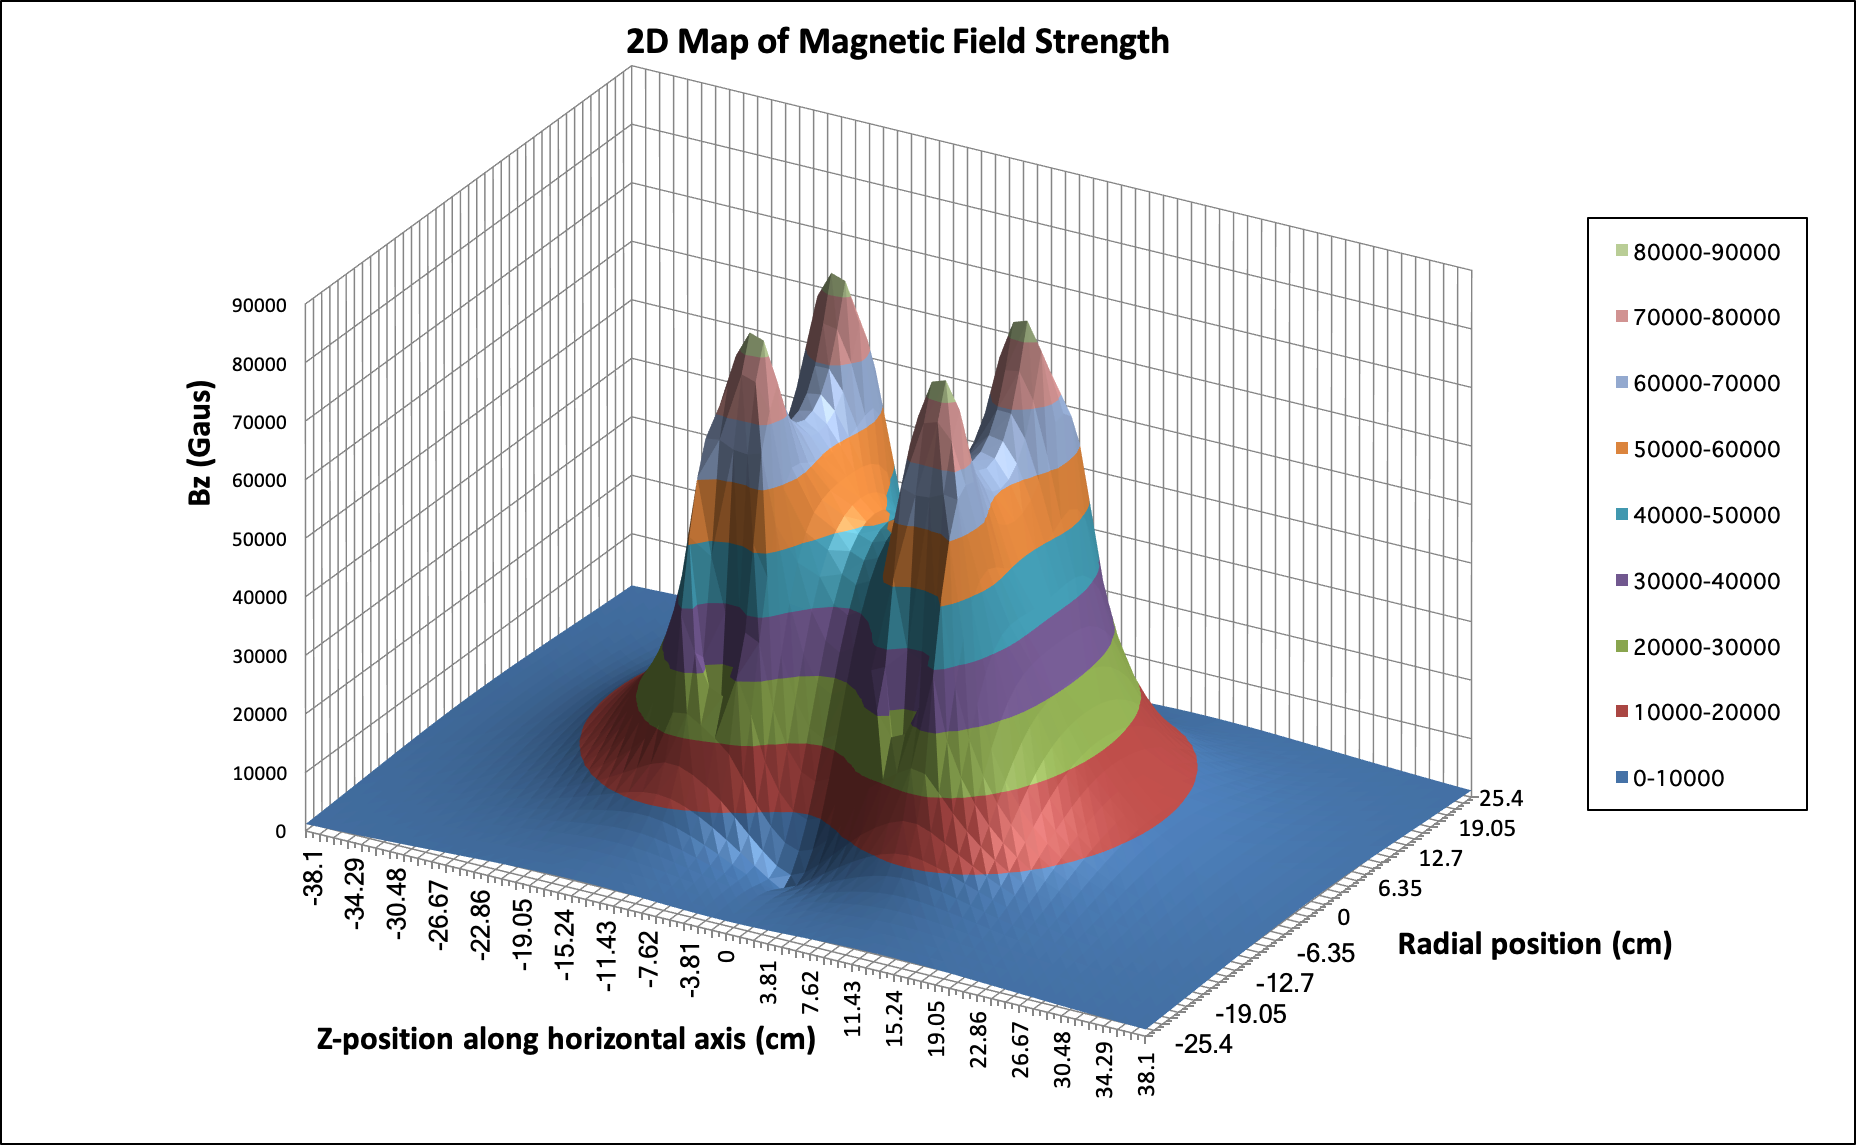
\includegraphics[width=0.9\textwidth]{target_field_map.png}
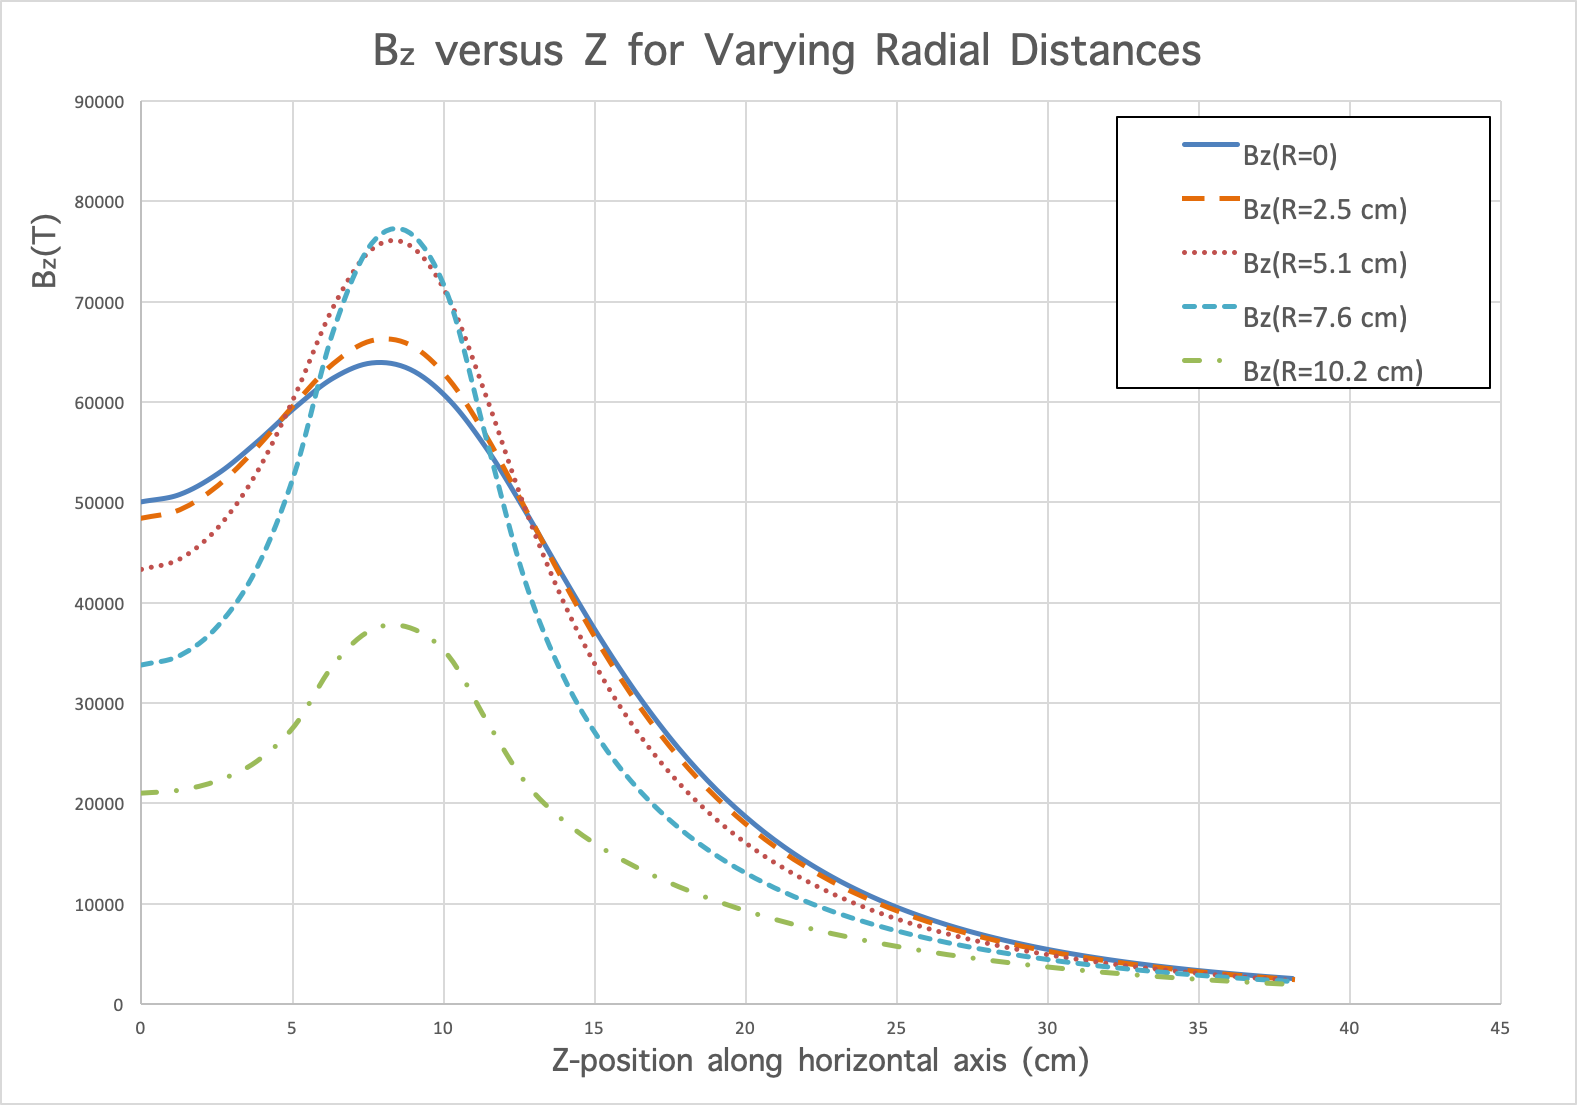
\includegraphics[width=0.9\textwidth]{BzvsZvarR.png}
\caption{\label{fig:tgt_field}Plots of manufacturer-provided magnetic field map at maximum current producing 5~T at the coil center shown in 2D (top) and 1D (bottom)}
\end{figure}
\subsubsection{Quadrupoles}
Four quadrupoles are used to focus the envelope of the events of interest through the dipole slits. The three most downstream quadrupoles (now termed Q2, Q3, and Q4 where the number increases as one moves down the beamline) are vintage optical elements originally obtained in the 1990's from LANL. These were given names Patsy, Tessa and Felicia respectively and were the only quadrupoles in the original design. During the Jefferson Lab upgrade to 12 GeV, a fourth dipole was added (now called Q1) in order to meet the higher energy requirements. 

The two most downstream quadrupoles,  Tessa and Felicia (Q3 and Q4) are of identical design and were mapped prior to their arrival at Jefferson Lab from LANL. Patsy (Q2), a slightly longer quadrupole was also mapped prior to arrival at Jefferson Lab. Q1 was designed at Jefferson Lab based on the design of Q3 and Q4. Measurements of the gradient-length (GL) versus current for each of the magnets were taken with a stretched wire \footnote{GL=$\int \mathbf{G} \cdot d \mathbf{l}$  where G is the gradient with respect to $r$, the radial distance and $l$ is along the wire which is parallel to the quadrupole z-axis and a fixed distance from it.}. These measurements are used to parametrize their non-linearity with respect to current. A simple 5 degree polynomial parametrization works well and is utilized in the GEANT4 simulation. Figure \ref{fig:GLparam} shows the GL cSaturation effects are most obvious for Q3 and Q4 with Q2 being the most linear, that is, suffering the least from saturation roll off near the maximum current.

Measurements of the higher order multipole contributions were made for each of the quadrupoles. These were made with standard techniques using a rotating wire coil. Q2, Q3 and Q4 measurements were made at LANL in 1996 and the new quadrupole Q1 was measured at Jefferson Lab in 2012. The higher order multipole contributions of for Q2, Q3 and Q4 were measured to be negligible ($<$1\% extrapolated to the pole tip at $r=5$~cm). The new quadrupole Q1 only has a significant higher order contribution from the dodecapole term and even that is only 1.5\%of the quadrupole contribution at 3.7~cm where it was measured. This turns into  5\% when extrapolated to the pole tip; however, since it is the farthest upstream quadrupole, its proximity to the target under typical operating conditions limits electrons in the acceptance to radii much less than the pole tip radius. Thus, this higher order contribution does not significantly effect the spectrometer behavior.
\section{Key Systematic Errors}

Although Eq. \ref{eq:A_LR} presents a straightforward prescription for determining the beam polarization if $A_{zz}$ and $P^{targ}_l $ are known, in general, neither of these two values are straightforward to calculate and end up being key sources of systematic error for M\o ller polarimetry.  Calculation of $A_{zz}$ requires calculating the detector acceptance, which involves a full simulation of the device and assessment of systematic error arising from inaccuracies in the optical model. Furthermore, non-uniform sampling of target atomic electrons in the acceptance of the detector gives rise to the so-called Levchuk correction, which in addition to corrections from multiple scattering and radiative corrections add additional complication to calculating $A_{zz}$. Calculating $P^{targ}_l$ requires accurate knowledge of the saturation magnetization of the target material and a precise method of extracting the pure spin component from this. It also involves assessment of uncertainty from target misalignment with the applied magnetic field and corrections for foil temperature and magnetic field strength. The remainder of this paper is dedicated to addressing the approach in Hall A to determining these values and the current assessment of systematic error. Current shortfalls will be addressed and suggestions for dealing with them provided.
\subsection{Calculating $A_{zz}$}
As previously mentioned, $A_{zz}$ is the acceptance-weighted longitudinal analyzing power $A_l$ (Eq. \ref{eq:analyzing_pow}) and, thus, determining it requires simulating the polarimeter. Furthermore, effects such as multiple scattering, radiative losses and the Levchuk effect which occur in the target must be accurately simulated and propagated through the spectrometer. We will start with an overview of the simulation and discuss its level of agreement with data.
\subsubsection{Simulation overview}
Here we discuss the details and maturity of the G4 simulation including
\begin{itemize}
\item{Overview of optical elements included and how each is known. Uncertainties and unknowns such as the width of the collimator opening and the dipole slits should also be included.}
\item{The fields of the magnetic elements. Do we use ideal or models or measured maps? If both are available which is most reliable? }
\item{Comparison to data. How do our rate scans look? Why might the normalization be wrong? }
\item{Sensitivity to misalignment of beam and optics.}
\item{Show the broken left-right asymmetry that comes from the solenoid, explain its origin and why we don't care about it.}
\end{itemize}
\subsubsection{Dealing with optics model uncertainty}
As previously discussed the absolute knowledge of the transfer optical matrix between the target and the detector has rather large uncertainties of order a few percent. This uncertainty has been traced to a combination of incorrect field assignments, misalignment of optical elements and incorrect beam orbit. Each of these is exacerbated at low beam energies such as the 1~GeV beam used by PREX-2. At the high energies of MOLLER (>10~GeV) these effects are expected to be much less significant. At the 1-2~GeV energies for PREX-2 and CREX the following procedure was demonstrated to reduce our sensitivity to knowledge of absolute optics settings. At these low energies, the four quadrupoles provided an under-constrained system with numerous possible quadrupole current settings that would provide nearly the same $\theta$ distribution of events on the detector. Possible solutions were shown using everything from a single quadrupole to all four with slight differences in expected rates. Eventually a solution was chosen using quadrupoles 1, 2, and 4 (from here on referred to as Q1, Q2 and Q4 respectively) and leaving Q3 off. Even this limited set had a number of possible configurations that could produce what appeared to be equal solutions. Qualitatively this meant that if one quadrupole current level were changed the other two could be adjusted to essentially zero out the change. Simulation suggested this flexibility could be leveraged to achieve insensitivity to absolute knowledge of the optics as long as the setup was calibrated by tuning relative to a calibration feature. For PREX-2 and CREX setups, this feature was chosen to be the rate maximum in the curve of detector coincidence rate versus Q1 current. Quadrupoles 2 and 4 were set to their nominal values provided by simulation. Next the current in Q1 was scanned mapping out the detector coincidence rate versus Q1 current. The final current setting for Q1 was determine relative to the current at rate maximum. Figure \ref{fig:uncQ2Q4} shows the simulated rate and $A_{zz}$ curves versus Q1 current when Q2 and Q4 are varied by $\pm$5\% around their nominal setpoints. The 1$\sigma$ width of the distribution of $A{zz}$ is less than XX\%. This prescription will be further examined in the next section on the Levchuk correction.


\begin{figure}[ht]
\centering
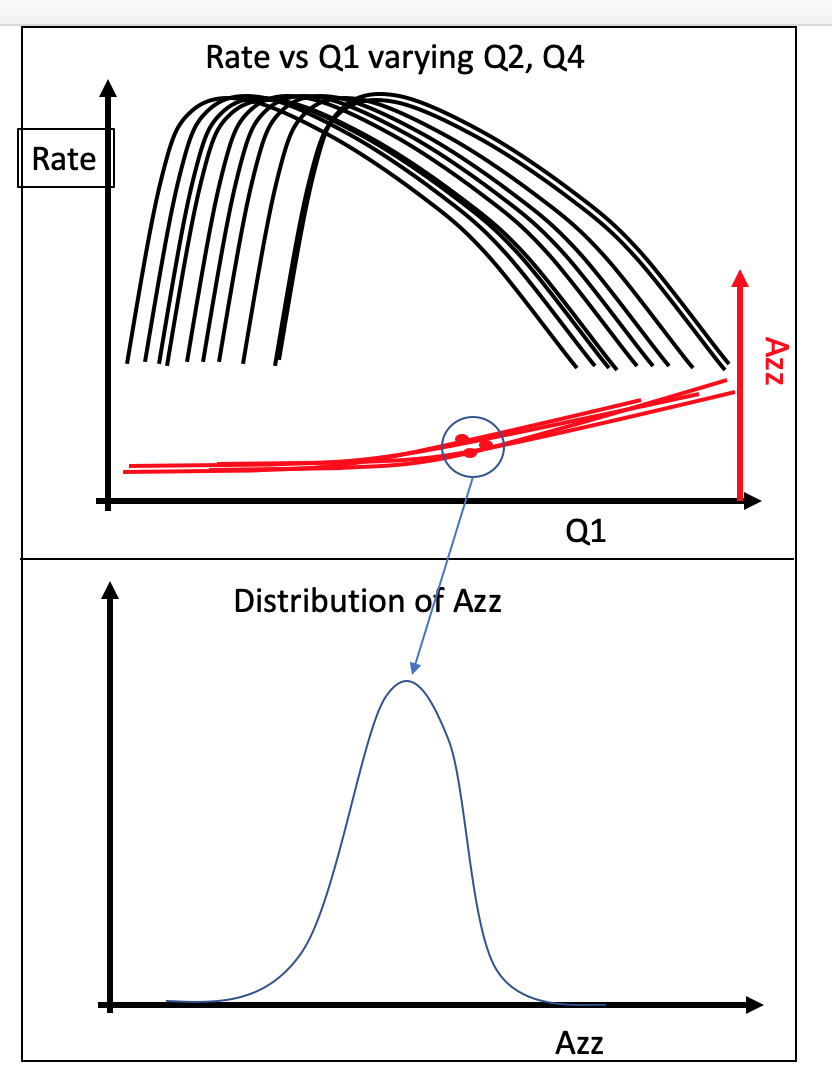
\includegraphics[width=0.7\textwidth]{AzzUncQ2Q4var.png}
\caption{\label{fig:uncQ2Q4}Top: Change in detector rate and $A_{zz}$ versus Q1 current for $\pm$5\% around the nominal setting for Q2 and Q4 currents.  Bottom: Distribution of $A_{zz} $when the setpoint for Q1 is chosen relative to the point at the maximum detector rate.}
\end{figure}
\subsection{Levchuk}

\begin{figure}[ht]
\centering
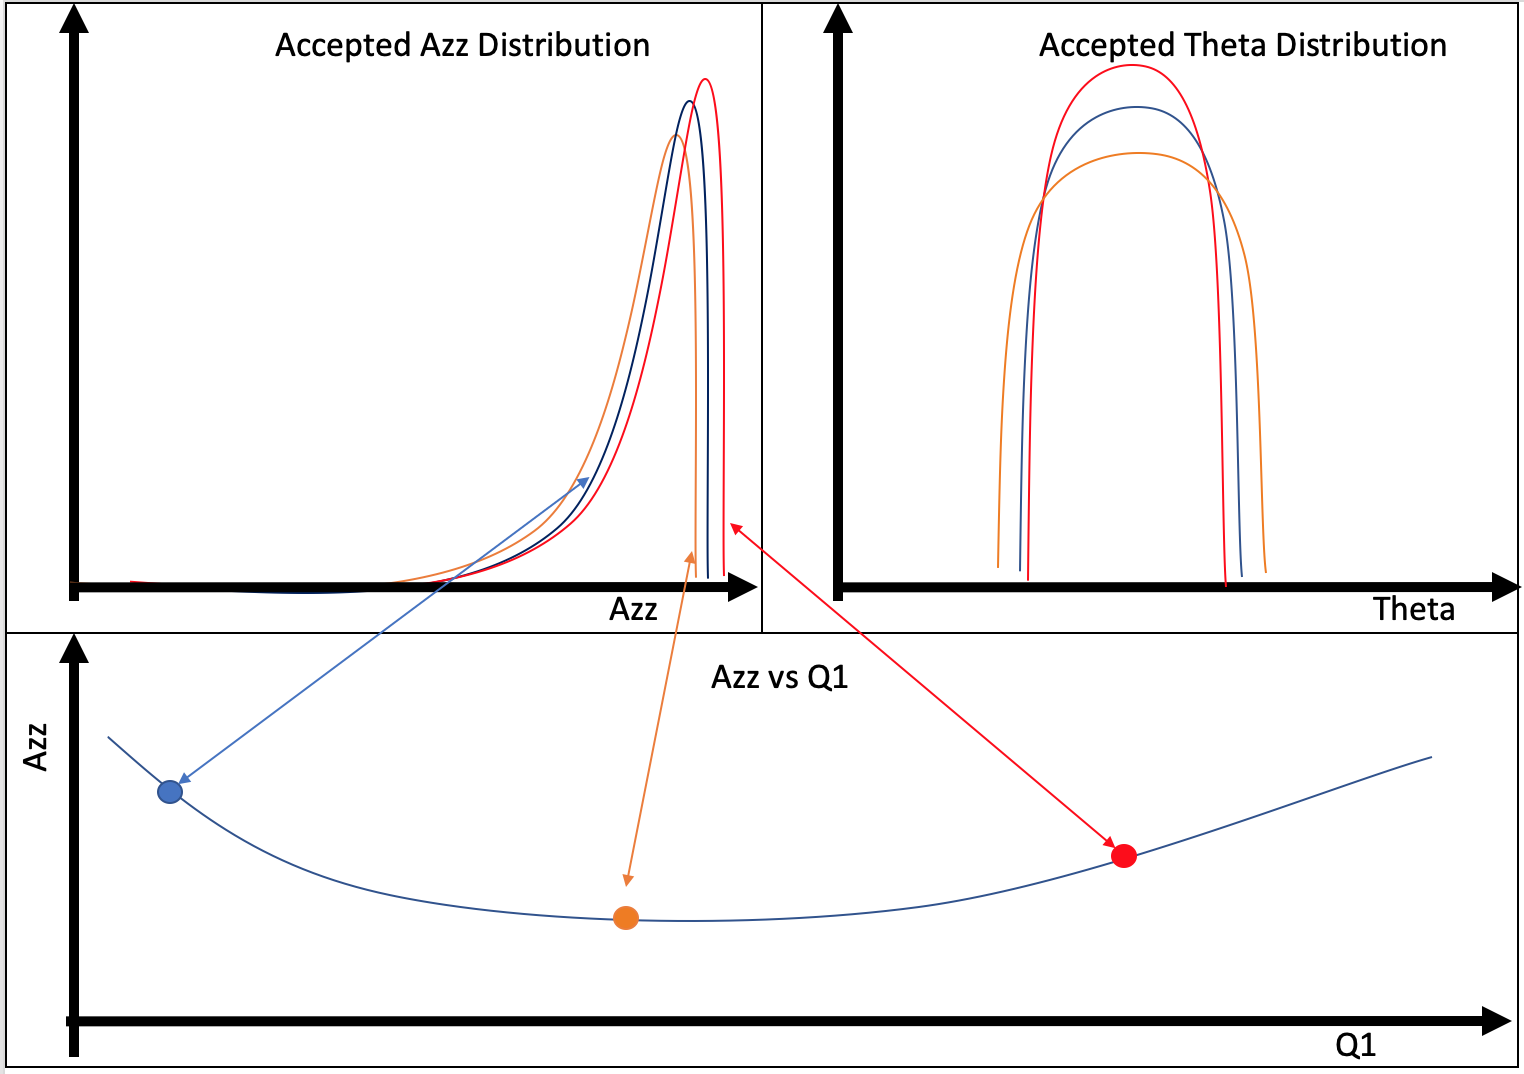
\includegraphics[width=0.7\textwidth]{AzzvsQ1.png}
\caption{\label{fig:AzzvsQ1}Azz and $\theta$ shown for various settings of Q1 current.}
\end{figure}
\begin{figure}[ht]
\centering
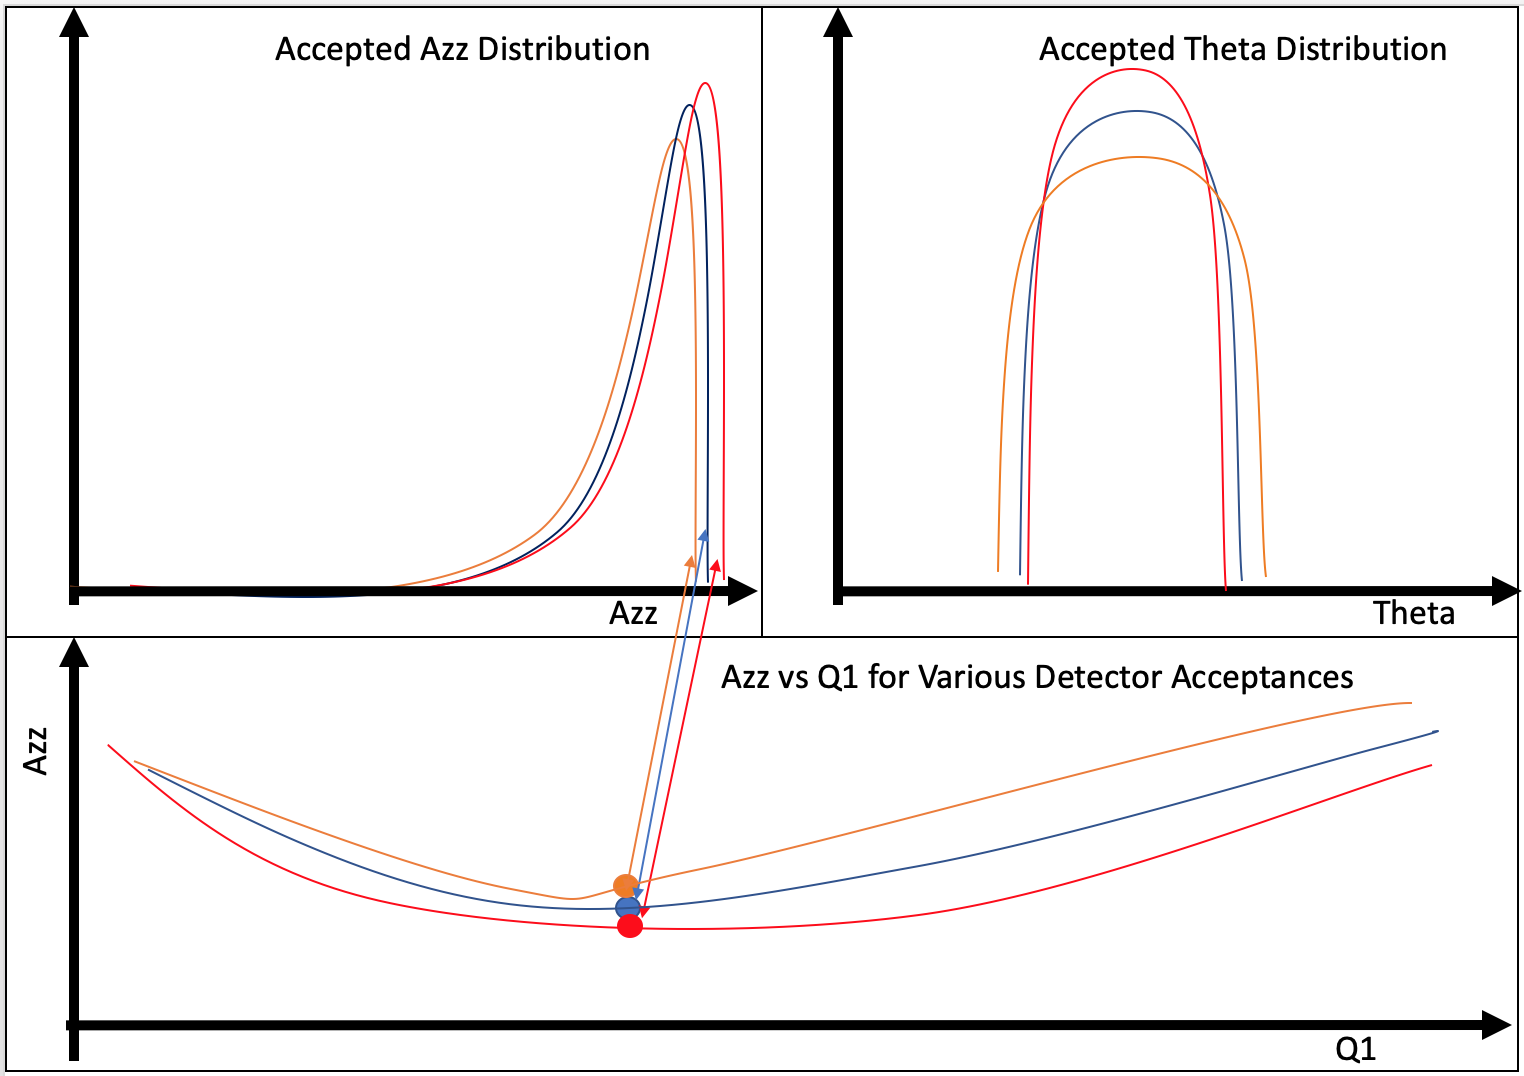
\includegraphics[width=0.7\textwidth]{AzzvsAcceptance.png}
\caption{\label{fig:AzzvsAcceptance}Azz and $\theta$ shown for various choices of momentum acceptance in the detector at CREX energies.}
\end{figure}



\section{Foil Target Polarization}
The M\o ller polarimeter target consists of a set of thin foils magnetized out of plane parallel (or antiparallel) to the beam trajectory. The three ferromagnetic elements, Fe, Co and Ni are the obvious choices due to their relatively high magnetization and the precision with which their magnetization is known. The default foil of choice has thus far been pure iron since its magnetization is known with the least relative error and because it has a relatively high Curie temperature, making it less sensitive to beam heating effects.
\begin{table}[h]
\begin{center}
\begin{tabular}{|r|l|l|l|}\hline
~&Fe&Co&Ni\\\hline
Z&26&27&28\\
Atomic Mass ($\mu$)&55.845(2)&58.933194(4)&58.6934(4)\\
Electron Configuration&[Ar]$4s^23d^6$&[Ar]$4s^23d^7$&[Ar]$4s^23d^8$ or $4s^13d^9$\\
Unpaired Electrons&2.2&1.72&0.6\\
Density near r.t. (g/cm$^3$)&7.874&8.900&8.902\\
$M_o$ at 0 K (emu/g)&222&164&58.6\\
$g^{\prime}$&1.92&1.85&1.84\\
Curie Temperature (K)& 1043&1400&358\\\hline
\end{tabular}
\end{center}
\caption{Properties of the three ferromagnetic elements.}
\end{table}

Although the magnetization of Fe and Ni are both known to high accuracy ($\sim0.2$ emu/g), since the magnetization of Fe is 3 to 4 times larger, the relative error is smaller. The low Curie temperature of Ni makes it susceptible to large (percent level) corrections from target heating effects. There are fewer published measurements of high precision on Co than on the other two ferromagnetic elements.

M\o ller polarimetery requires finding the average target electron polarization; however, magnetization measures the magnetic moment of the whole atom including the orbital and spin magnetic moments. Since we only want the spin component we need to find the fraction of the magnetization that comes from spin. This is typically determined from precise measurements of the gyromagnetic ratio of an elemental sample. Thus, the final error on the target polarization will include uncertainties on both the determination of magnetization and of the spin component.

In the following sections I look at each of the three elements and determine what the total uncertainty would be if we used each of the three ferromagnetic elements as our target.

The issues facing us are follows:
\begin{itemize}
\item{Through the years from 1930-1980 many precise measurements have been made of the magnetization and gyromechanical properties of these elements; however, they do not necessarily agree within error. Sometimes the errors quoted are not realistic given the systematic disagreement in the data. The sources of systematic difference are often not known and yet results are averaged together and the final error quoted as the statistical variation.}
\item{No mention is made of the nuclear contribution to the magnetic moment. The nuclear magneton is smaller than the Bohr magneton by a factor of $m_e/m_p\sim0.05\%$. Fortunately, the main isotopes that make up iron and nickel are even-even and have spinless nuclei, but for Co the average is 4.6 nuclear magnetons taking us above the 0.1\% level we care about.}
\item{How well do we know the corrections needed to take us from the field and temperature values in the literature to the conditions in our polarimeter?}
\item{Through the past century measurement of constants have become more precise and have changed. Examples of constants used in determining quoted magnetization and gyromagnetic data in the literature are the density of elements, the charge to mass ratio of the electron, and the Bohr magneton. Different groups use different values. How can an appropriate uncertainty be assigned for this?}
\item{Experiments measuring properties of these ferromagnetic elements used different levels of purity. What level of uncertainty should be assigned to account for the effects of impurities?}
\end{itemize}

\
%\centering
%\captionsetup{width=5in}
%\includegraphics[width=5in]{}
%\caption{ Fractional }
%\label{fig:Xubo_spectrum}
%\end{figure}

\subsection{Determining Magnetization}\label{method}
Target polarization is determined from measurements of the saturation magnetization of pure iron. Another term used in the literature is ``spontaneous magnetization'', which as the name implies refers to the magnetic moment of a material that spontaneously arises with no applied field. In ferromagnetic materials the magnetic moments of the electrons tend to spontaneously align in a given direction. However, due to energy considerations, domains which are small regions of aligned spin, tend to form in such a way so that the total spin averaged across many domains at the macroscopic level is far below the saturation level and may be zero. In the presence of an applied magnetic field, the domain boundaries shift with enlarging domains with magnetic moments aligned along the direction of the field. As the applied field is increased, eventually the material will reach magnetic saturation where all the spins are aligned along the direction of the applied field. Thus, the saturation magnetization and the spontaneous magnetization are numerically equal although the spontaneous magnetization cannot be measured at room temperature due to domain formation. 

Spontaneous magnetization is a function of temperature and applied field and for this reason it is often given as $M_{0}$, the value of saturation magnetization extrapolated to zero applied field at T = 0~K. However, experiments measure the magnetization at temperatures above 0 K with applied fields. For temperatures well below the Curie temperature and low applied fields, the magnetization has been shown to roughly follow the $T^{3/2}$ law of Bloch given as \cite{Bloch1930}
\begin{equation}
M_s(T) = M_0(1-a_{3/2}T^{3/2}),
\label{eq:bloch}
\end{equation}
where $M_0$ is the saturation magnetization at 0 K and $a_{3/2}$ is an empirically determined constant. At higher fields and temperatures not small compared to the Curie temperature additional terms are required\cite{PauthenetNov1982}. Pauthenet expresses the magnetization as a function of temperature and applied field as follows:\cite{PauthenetMar1982,PauthenetNov1982}
\begin{equation}
M_s(H_i, T) = M_s(T)+A(T)H_i^{1/2}+B(T)H_i,
\label{eq:pauthenet}
\end{equation}
where $M_s$ is given by Eq \ref{eq:bloch} and A(T) and B(T) are functions of temperature and can be extracted from fits to data of magnetization versus internal field at a constant temperature. Pauthenet utilizes fits to his data to give a numerical expression for magnetization as a function of internal magnetic field and temperature (see Eq. 9, 10 and Table 1 from \cite{PauthenetMar1982}). Corrections for differences in temperature and internal field made will come from Eqs. 9 and 10 in \cite{PauthenetMar1982}.

It is important to note the difference between internal field and applied field. In a manner somewhat analogous to the internal electric field cancelation inside a dielectric, the applied magnetic field is partially cancelled inside a ferromagnetic sample. This can be viewed as being caused by magnetic charges moving to the boundaries of the sample in accordance with the direction of the magnetic field. Their displacement will enhance the field outside the sample while reducing it inside. The relationship between the internal field and the applied field is given by the following equation (in the cgs system)
\begin{equation}
H=H_i+\frac{4\pi M}{\rho},
\end{equation}
where $H$ is the applied field, $H_i$ is the internal field, $M$ is the magnetization and $\rho$ is a demagnetization constant that depends on the shape of the sample. Since the internal field is thus partially cancelled by the magnetization, $4\pi M$ is sometimes referred to as the ``demagnetizing field''. 

Well below saturation, the internal field is nearly 0 due to the demagnetizing field. Field-dependent corrections are calculated as a function of internal field $H_i$ not applied field $H$. There appear to be errors in the literature that stem from incorrect exchanges of applied field and internal field. For example, Eq. 3 from deBever {\it et al.} incorrectly interprets Pauthenet's corrections as a function of flux density $B$ instead of internal field. As a result, they calculate a correction from an applied field of 1~T to the final value of 4~T. Their 4~T applied field translates into an internal field of $\sim$1.8~T for Fe foils, requiring a smaller correction. C. D. Graham also appears to confuse the two in Fig. 5  of \cite{Graham1982} where he plots magnetization versus $1/H$ but combines data from multiple sources some of which are in terms of $1/H$ and others which are in terms of $1/H_i$.  


 Thus, the magnetization of an object at a particular temperature and applied field is not just a function of its elemental composition. Other factors that affect the magnetization are
\begin{itemize}
\item{Shape anisotropy: the magnetization depends upon the shape of the object. Needles are very easy to magnetize along their long axis but much more difficult along a direction perpendicular to it. Each shape has a characteristic demagnetizing factor that is a function of the direction of applied field (unless symmetry dictates otherwise). Perfect spheres have a demagnetizing factor of 3. The demagnetizing factor for ellipsoids of rotation is a function of the ratio of the two axis lengths. Figure \ref{fig:demag_ellipsoid} shows the demagnetizing factor of ellipsoids of rotation as a function of the axis ratio where the applied magnetic field is along the axis $R_z$. A thin foil disk such as that used in the M\o ller polarimeter can be taken to a flattened ellipsoid with an axis ratio of $\sim$0. In this case the demagnetizing factor approaches unity.}
\item{Crystal anisotropy: the crystal structure of a material can create directions along which it is easier to magnetize. The direction along which magnetic saturation is reached with the smallest applied field is called the easy axis of the crystal. Monocrystalline nickel, for example, has three different magnetization axes termed the [111],[110] and [100] axes with [111] being the easy axis. Thus, if you are using monocrystalline materials, the magnitude of the external field required to reach saturation will depend upon alignment of the crystal relative to the field. For polycrystalline materials there will be no preferred direction due to crystal structure.}
\item{Crystal structure and phase changes: some crystals have more than one possible crystal structure with different magnetizations. Their history of heating/cooling and annealing can have an effect on their magnetic properties. Cobalt, for example, goes through a phase change when heated at 690~K going from a close-packed hexagonal to a face-centered cubic crystal structure above 690 K which is unstable below that temperature. However, the exact crystal structure below 690 K (and by extension the magnetization) depends upon the grain size and the annealing process used to prepare it \cite{Owen1954}.}
\item{Magnetic history: due to remanence, a ferromagnetic sample may have nonzero magnetization with no applied field. Thus, the magnetization versus applied field curves will depend upon the value of the magnetization at 0 applied field and the history of previously applied fields.}
\item{Stesses and strains: stresses and strains in the material as well as porosity will affect how easily the material is magnetized. This can be seen particularly well by annealing, which often makes the material more easily magnetized\cite{Case1966}.}
\end{itemize}
 
Although different methods are used to measure the saturation magnetization, they broadly break down into two categories. 
\begin{itemize}
\item{Force method: a small ellipsoid sample of the element of interest is placed in a precisely determined field gradient. With a proper setup, the force on the sample by the magnetic field can be shown to be the product of the magnetization and the magnetic field gradient. Thus the magnetization is given as the force divided by the field gradient.}
\item{Induction method: a sample is placed into a magnetic field and its presence creates a magnetic moment that is measured in pickup coils.}
\end{itemize} 
     
Although the experimental methods can be thus broadly categorized, each individual experiment takes a slightly different approach to measurement and calibration.
\begin{figure}
\centering
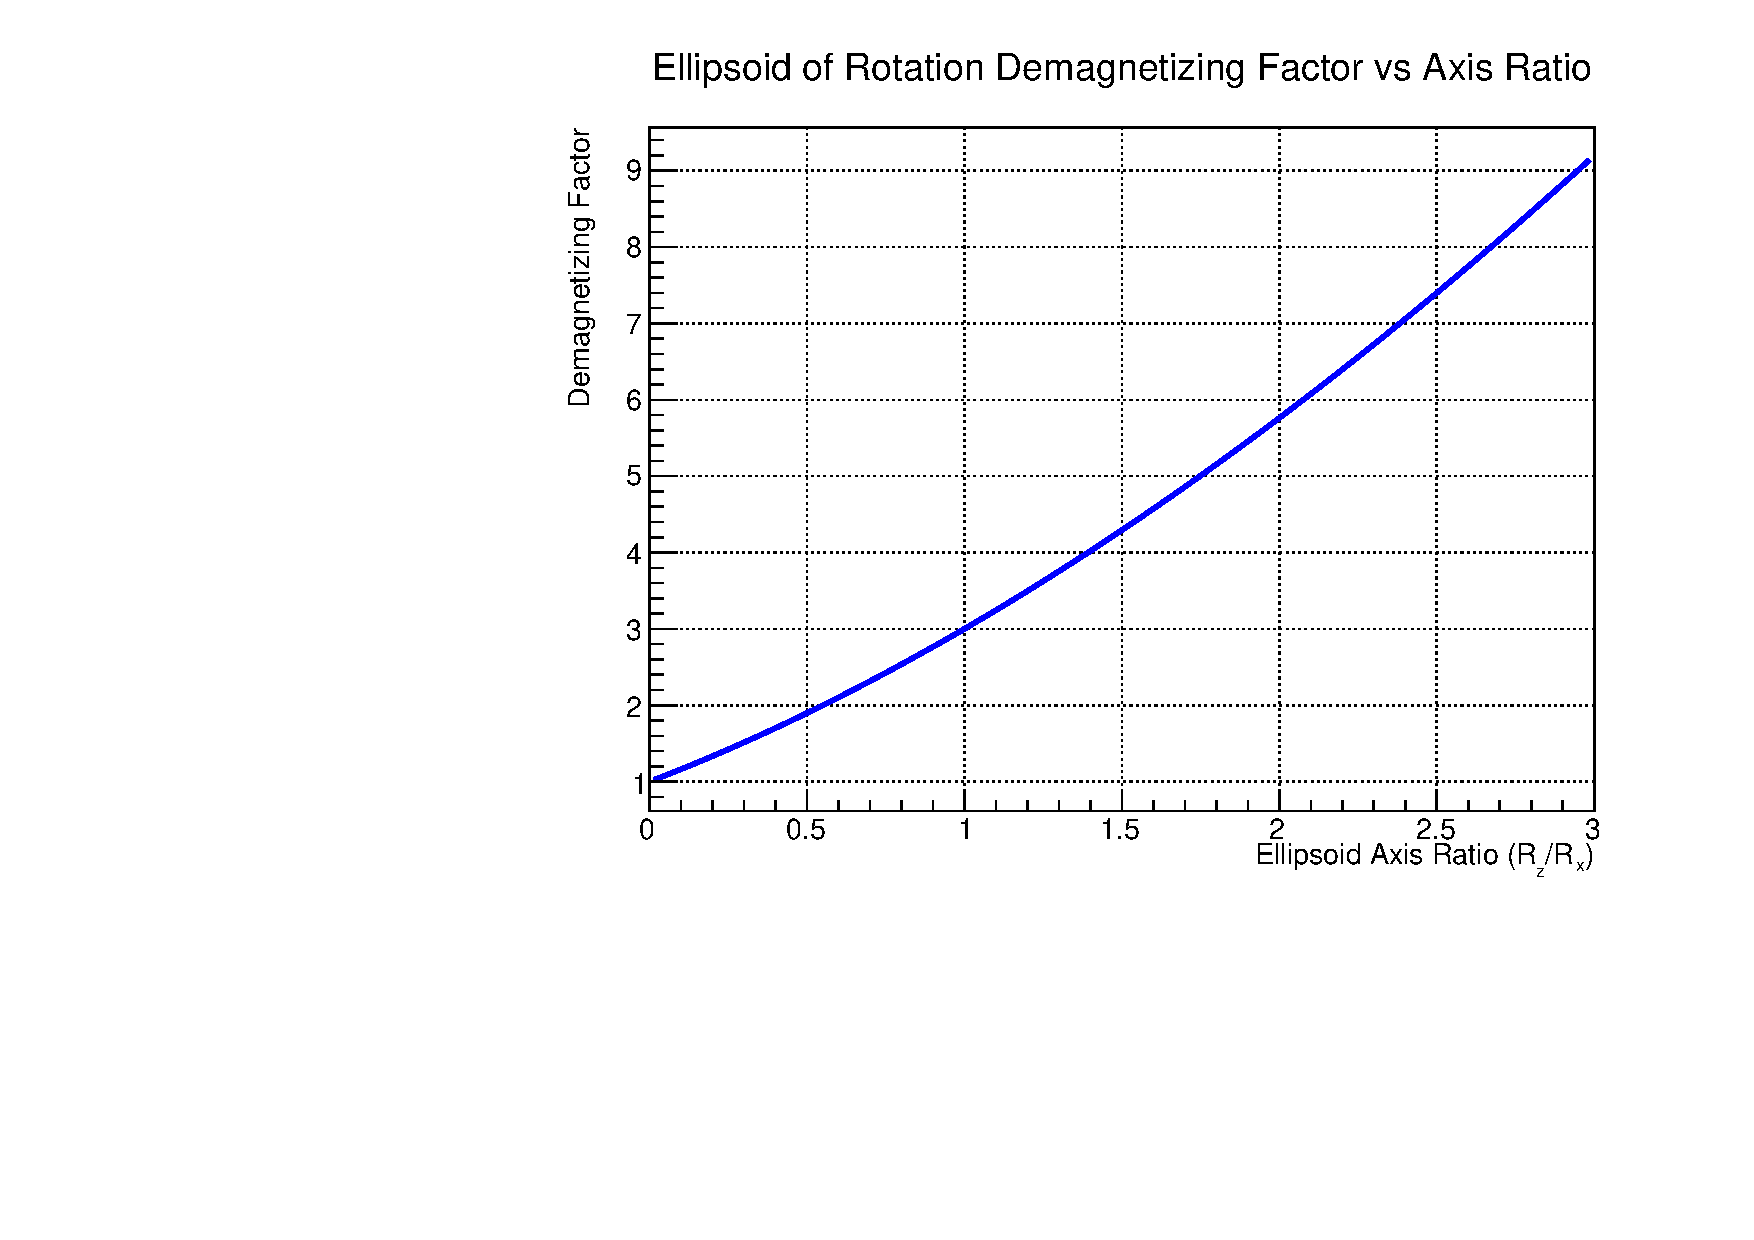
\includegraphics[width=0.7\textwidth]{demagnetizing_factor.pdf}
\caption{Demagnetizing factor for ellipoids of rotation as a function of axis ratio for external magnetic field applied along the axis of rotation $R_z$.}
\label{fig:demag_ellipsoid}
\end{figure}

Measurements of magnetization are performed at a variety of applied magnetic fields and temperature and are typically expressed in terms of the saturation magnetization $M_o$ which is the extrapolation to zero applied field at 0~K\cite{Crangle1971}. A review of the literature yields many measurements of the magnetization of iron and nickel. Different approaches can be taken to obtain ``consensus'' values. One approach taken by H. Danan {\it et al.}\cite{Danan1968} and deBever {\it et al.} \cite{deBever1997} is to average the values of spontaneous magnetization $M_0(H=0, T=0~K)$. A correction must then be applied to obtain the magnetization at room temperature and nonzero applied fields. However, the process of extrapolation to zero field and temperature is not standardized and different methods are utilized, so it is not clear that this is a good standard for comparison. Furthermore, since we are looking for magnetization near room temperature this method introduces error extrapolating down to $M_0$ and once again correcting back up to room temperature and high fields. Since most measurements at least include data at or near room temperature and at internal fields at or close to 10000~Oe (1~T), I chose to utilize magnetization measurement data taken near room temperature and internal fields of order 10~kOe. Where the available data in the literature were not available at precisely $T=294^{\circ}$K, small corrections were applied to the measurements based upon the formulation given in \cite{PauthenetMar1982}. In each case the data of magnetization versus internal magnetic field was parameterized using Eqs. 9 and 10 from \cite{PauthenetMar1982}. 

Although my ``consensus'' values for magnetization include data from a number of measurements done over a period from 1929-2001, this is not an exhaustive data set by any means. Table \ref{tab:magnetization_pubs} lists the publications used in this analysis for iron and nickel. In choosing data which data to include in my value for magnetization I used the following criteria:
\begin{itemize}
\item{Original data was published and publication was available. Some measurements referred to in the literature are not readily available. For example much of Danan's reported measurements on Ni were never published except in his 1968 review which provides few details of the experiment. I chose to used only those data for which I had access to the original publication.}
\item{Data in the publication was available near my chosen standard parameter values of $H_i=10$~kOe and $T=294~$K.}
\item{Enough details were provided to obtain the internal field of the sample either because the data were given versus internal field or the demagnetizing factor could be calculated from information given.}
\item{Sufficient information was provided about the purity of the sample used to ensure this will be a small source of error.}
\item{Systematic errors were sufficiently small to provide useful additional information. For example, Pauthenet \cite{PauthenetMar1982} has very precise data, but since he uses Danan's data for absolute calibration, his systematic error is 0.5\%. Aldred \cite{Aldred1975} also has a precise data set, but calibrates his data using the ``known magnetization of nickel'' which is exactly what I am trying to determine. Because of this I do not utilize these data in determining the absolute magnetization values.} 
\end{itemize}
\begin{table}[h]
\begin{center}
\begin{tabular}{|l|l|l|l|}\hline
Publication & Year & T ($^{\circ}K$) & Comment\\\hline
Weiss and Forrer \cite{Weiss1929} & 1929 & 288 & Only Fe data considered reliable\\
R. Sanford {\it et al.}(NIST)\cite{Sanford1941} & 1941 & 298 & Data on Fe only\\
H. Danan \cite{Danan1959} & 1959 & 288 & Data on Ni and Fe\\
Arajs and Dunmyre \cite{Arajs1967}& 1967 & 298 & Data on Ni and Fe\\
Crangle and Goodman \cite{Crangle1971} & 1971 & 293 & Data on Ni and Fe\\
Behrendt and Hegland (NASA)\cite{Behrendt1972} & 1972 & 298.9 & Data on Fe only\\
R. Shull {\it et al.}(NIST) & 2000 & 298 & Data on Ni only\\\hline
\end{tabular}
\end{center}
\caption{\label{tab:magnetization_pubs}Publications used in obtaining consensus value for magnetization near room temperature at high fields.}
\end{table}

Table \ref{fig:mag_Fe} shows the data for the magnetization of Fe from the published sources before and after correction to T=$294^{\circ}$K. The data cover different ranges of internal field, so to obtain an expression for the evolution of magnetization with internal field, I simply plot all the data together and fit it to the expression given in Eq 9 in \cite{PauthenetMar1982}
\begin{equation}
M(T,H_i)=M_0+aT^{3/2}F(3/2,bH_i/T)+cT^{5/2}F(5/2,b H_i/T)+\chi(T)H_i,~~\textrm{emu/g}
\label{eq:mag_vs_Hi}
\end{equation}
where a, b and c are constants found empirically to be $a=307\times 10^{-6}$, $b=1.378\times10^{-4}$\footnote{Note that Pauthenet uses $b=1.378$ for Fe in Eq. 9 of \cite{PauthenetMar1982} and $b=1.478$ for Ni in Eq. 10 of \cite{PauthenetMar1982}, but the only way I could replicate his plots in Figure 1 of \cite{PauthenetMar1982} and \cite{PauthenetNov1982} was to use  $b=1.378\times10^{-4}$ for Fe and $b=1.478\times10^{-4}$ for Ni. } and $c=-22.8\times10^{-8}$. F is given by $F(s,H/T)=\sum_{p=1}^{\infty}p^{-s}e^{-pg\mu_BH/k_BT}$ with $g$ the Lande g-factor, $\mu_B$ the Bohr magneton and $k_B$ the Boltzmann constant. $\chi(T)$ is the susceptibility as a function of temperature and its evaluation is given in Table 1 of \cite{PauthenetMar1982} for discrete values. In order to be able to evaluate $\chi(T)$ for any temperature, I fit a linear function to the data to obtain $\chi(T)\approx3.644\times10^{-6}+5.0434\times10^{-10}T$ which is the expression I use in evaluating equation \ref{eq:mag_vs_Hi}. I fit this expression to the data with $M_0$ and an offset in internal field as fit parameters. Note that the data for Weiss and Forrer and for Sanford {\it et al.} are given in the literature at a single value of $H_i$ even though they are composed of multiple values across a range of applied fields not included in the publication. To account for this I weighted these data points three times more than any single other point in the fit. 

The magnetization curve fit to the data is slightly sensitive to the range of data selected as well as to whether or not the 0 value of $H_i$ is allowed to float using an offset parameter. Fig. \ref{fig:mag_fit_Fe} shows the data for Fe along with four different fits of Eq. \ref{eq:mag_vs_Hi} to the data demonstrating the range of resulting curves for different conditions placed on the fit. The systematic error from the fit is small compared with the spread in the data. 

My suggestion is to take the average of the red and green curves (the two central curves) in Fig. \ref{fig:mag_fit_Fe} and to assign a conservative systematic error of 0.15\% based upon the spread in the data from many experiments with different systematic errors. This parameterization is shown in Fig.\ref{fig:mag_errorband_Fe}. Since the saturation magnetization of iron is approximately 2.2~T and the demagnetization factor is unity for a thin foil magnetized out of plane, the difference between the internal field is approximately 2.2~T less than the applied field near saturation. Thus a uniform external 4~T magnetic field corresponds to an internal field of approximately 1.8~T. Reading from Fig. \ref{fig:mag_errorband_Fe} gives the magnetization per gram for iron at 294$^{\circ}$K with an applied field of 4~T as $\sigma_{Fe}=217.95\pm0.33$ emu/g. This translates into $2.1793\pm0.0033~\mu_B/$atom which differs by nearly 0.2\% from the value of $2.183\pm0.002~\mu_B/$ determined by deBever {\it et al.}\cite{deBever1997} partially due to their over-correction for the magnetic field. 

A similar analysis of the literature for nickel is shown in Figs. \ref{fig:mag_Fe} to \ref{fig:mag_errorband_Fe}. The error band in Fig \ref{fig:mag_errorband_Fe} is $\pm0.14$~emu/g which is approximately 0.25\%.  Since the saturation magnetization of nickel is approximately 0.6~T and the demagnetization factor is unity for a thin foil magnetized out of plane, the internal field is approximately 0.6~T less than the applied field near saturation. Thus a uniform external 2~T magnetic field corresponds to an internal field of approximately 1.4~T. Reading from Fig. \ref{fig:mag_errorband_Fe} gives the magnetization per gram for nickel at 294$^{\circ}$K with an applied field of 2~T as $\sigma_{Ni}=55.20\pm0.14$ emu/g, which translates into $0.5801\pm0.0015~\mu_B/$atom.
\begin{figure}
\centering
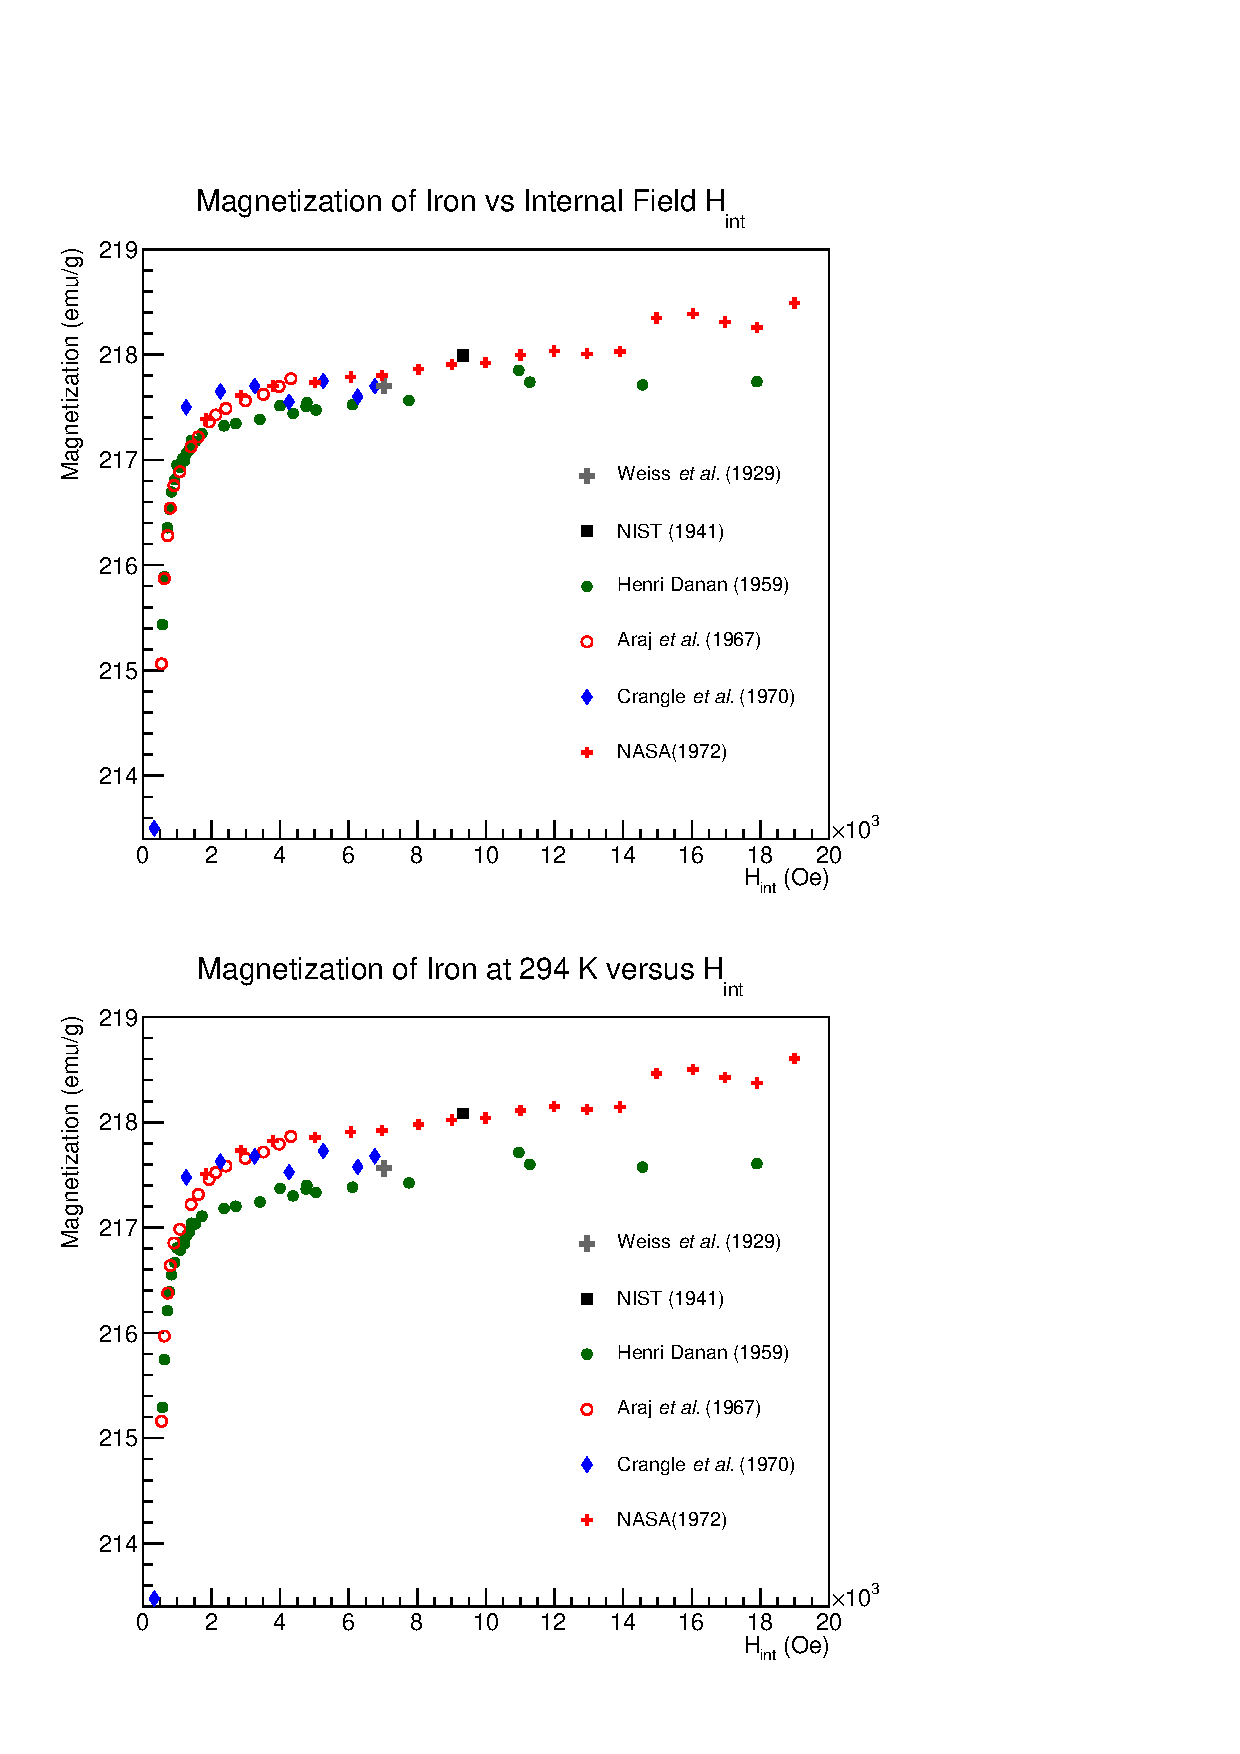
\includegraphics[width=0.64\textwidth]{FeMagnetization_vs_Hint.pdf}
\caption{Published magnetization data from various sources for Fe shown versus internal field. The top plot shows data for temperature at which it was taken and the the bottom plot shows the same data corrected to 294$^{\circ}$K. }
\label{fig:mag_Fe}
\end{figure}
\begin{figure}
\centering
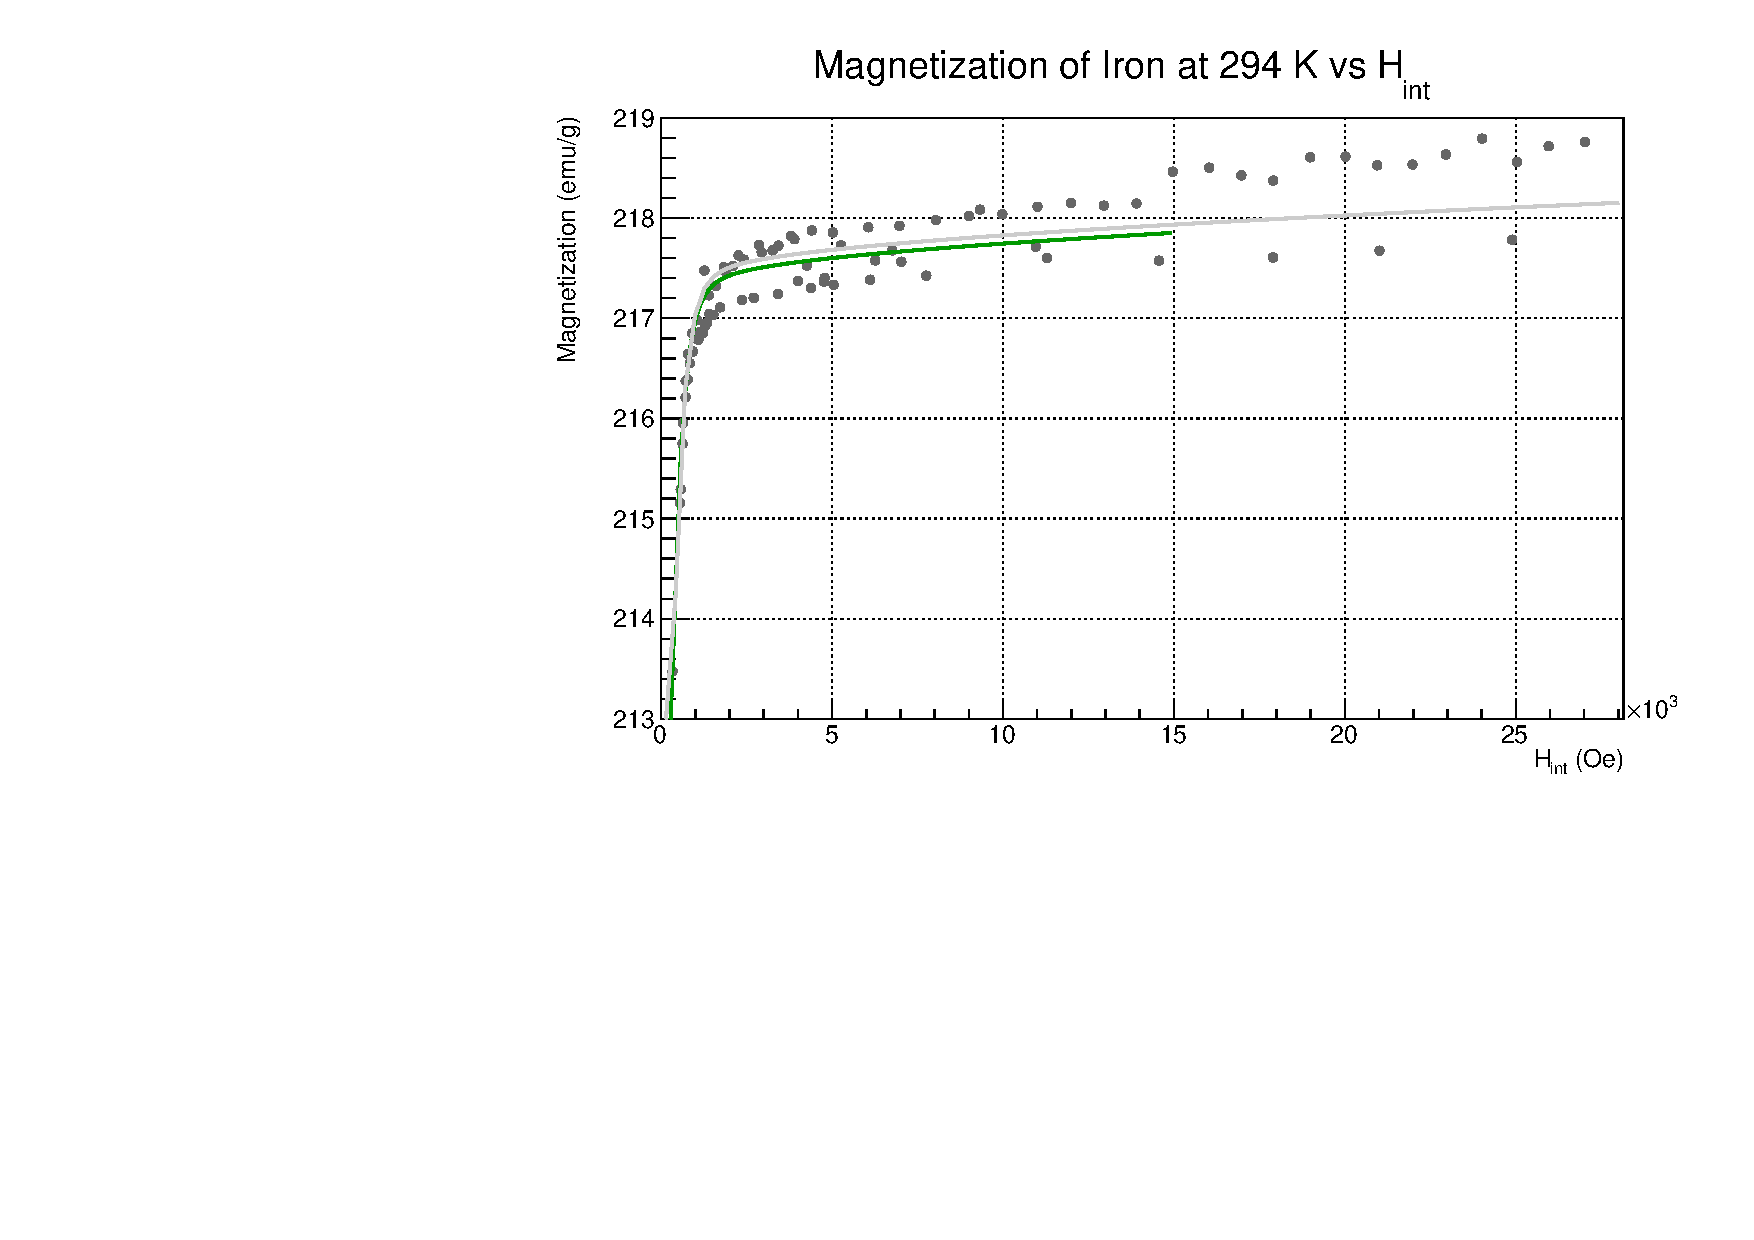
\includegraphics[width=0.7\textwidth]{FeCombinedFit_vs_Hint.pdf}
\caption{Fits to magnetization data using Eq. 9 from \cite{PauthenetMar1982}. The different results demonstrate the systematic uncertainty associated with using this parameterization. The blue line represents a fit over the range 1-20 kOe with the saturation magnetization as a single fit parameter. The remaining fits utilize an additional fit parameter allowing the 0 of the ordinate to float but with different ranges of data fit as can be seen in the figure.}
\label{fig:mag_fit_Fe}
\end{figure}
\begin{figure}
\centering
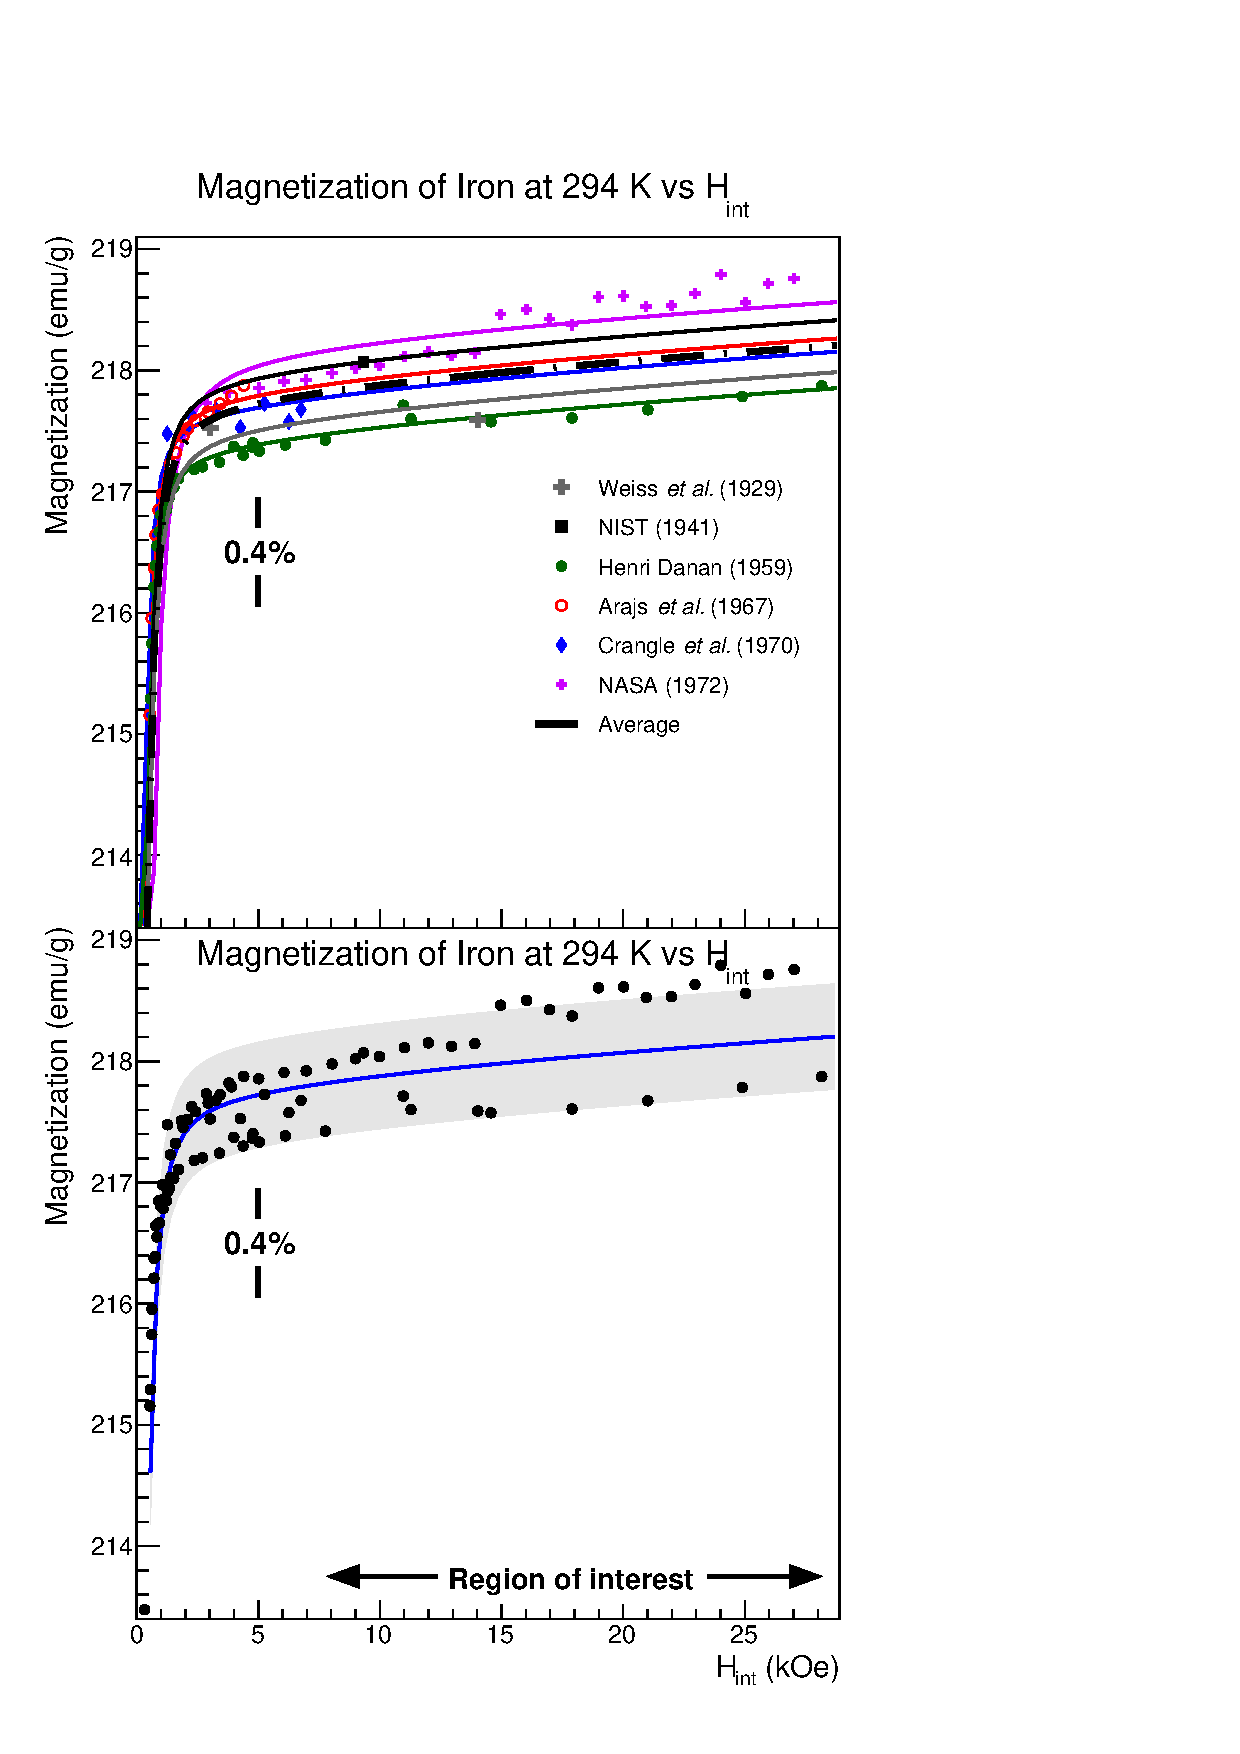
\includegraphics[width=0.7\textwidth]{FeCombinedFitErrorBand_vs_Hint.pdf}
\caption{Published magnetization data from various sources for Fe plotted versus internal field corrected to 294$^{\circ}$K and shown with proposed parametrization curve for internal fields up to 20~kOe (2~T). The curve is approximately the average of the two central curves in Fig. \ref{fig:mag_fit_Fe}. For a thin iron foil magnetized out of plane (normal to the surface) close to saturation, the difference between the internal and applied field is about 2.2~T so 4~T external field corresponds to 1.8~T (18000 Oe) internal field. The error band corresponds to 0.33 emu/g or $\sim$0.15\%. }
\label{fig:mag_errorband_Fe}
\end{figure}


\begin{figure}
\centering
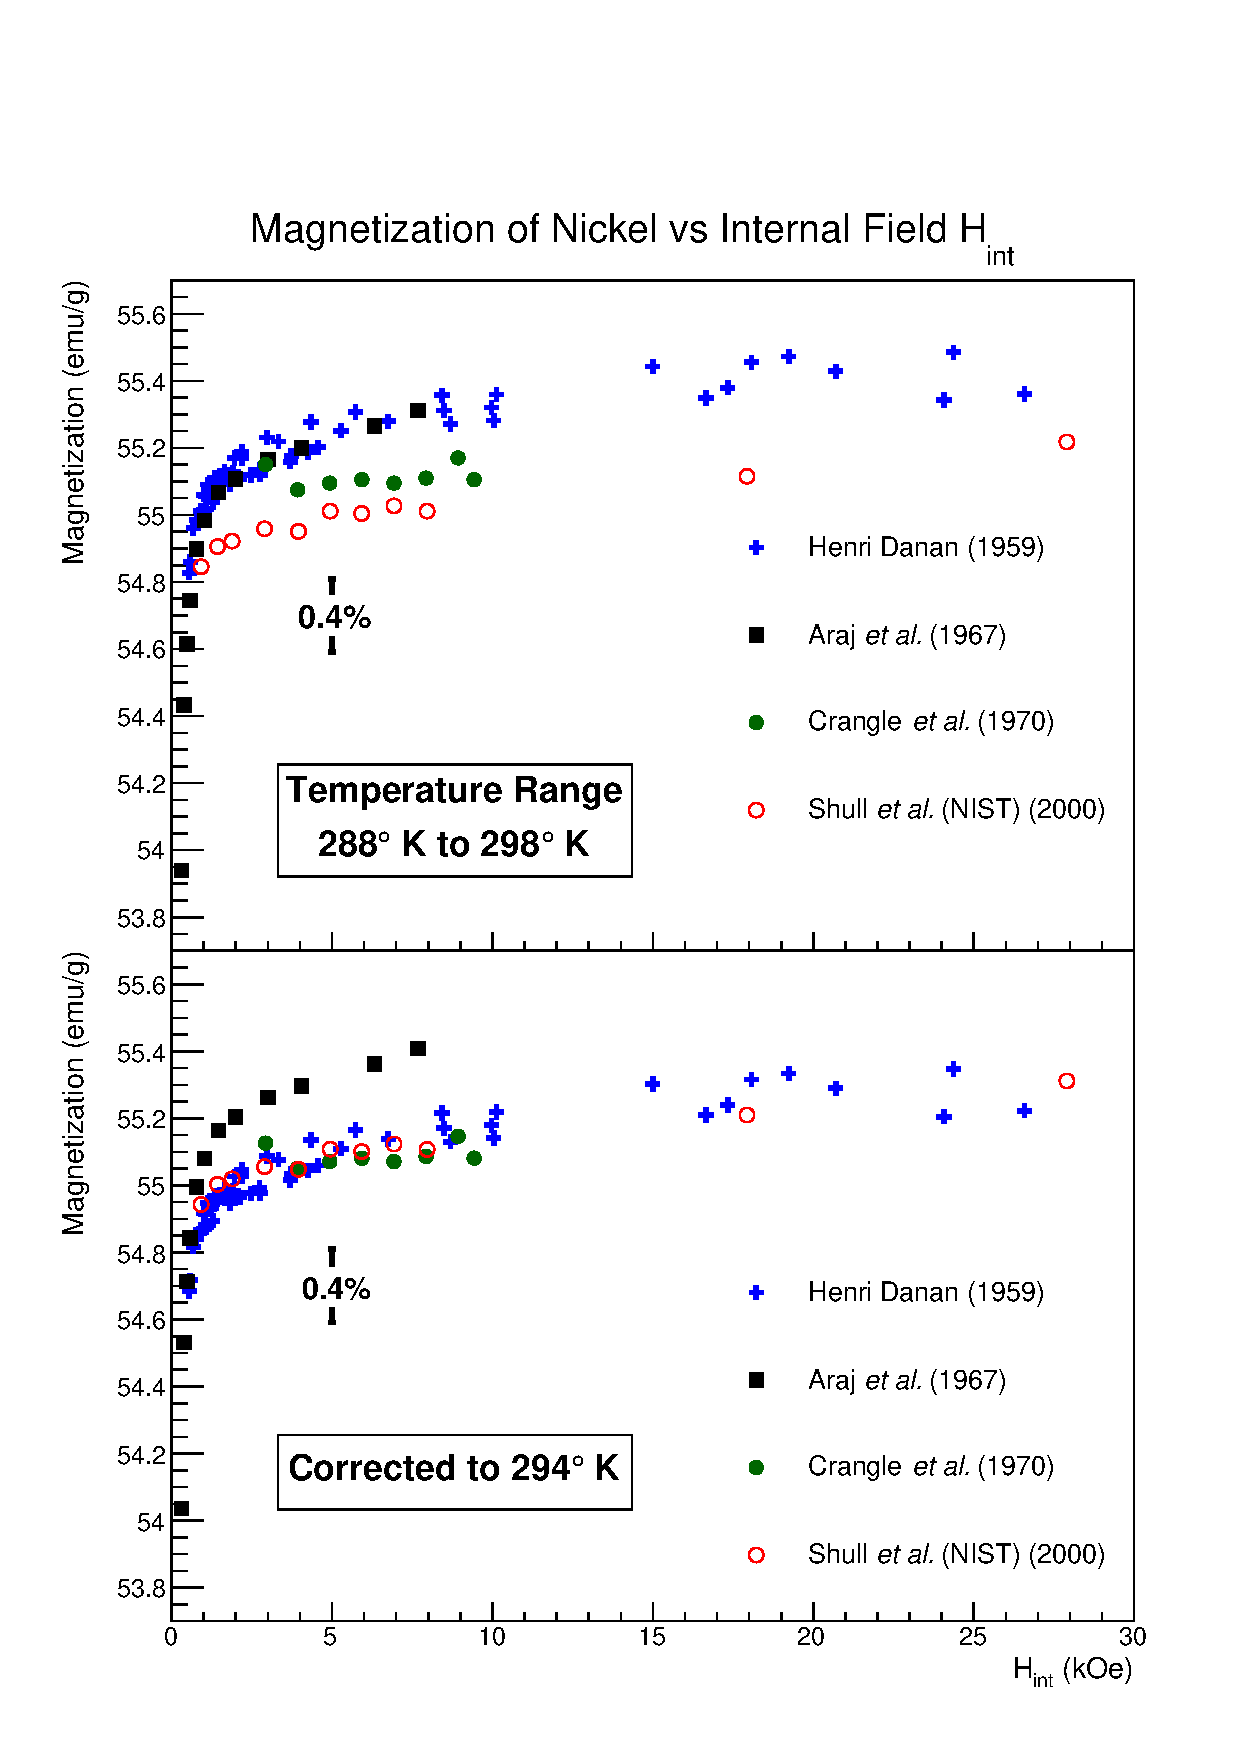
\includegraphics[width=0.64\textwidth]{NiMagnetization_vs_Hint.pdf}
\caption{Published magnetization data from various source for Ni shown versus internal field. The top plot shows data for temperature at which it was taken and the the bottom plot shows the same data corrected to 294$^{\circ}$K. There is good agreement in the data with the clear exception of that from Arajs {\it et al.} which are systematically higher by $\sim0.5\%$. The reason for this discrepancy is not clear.}
\label{fig:mag_Ni}
\end{figure}
\begin{figure}
\centering
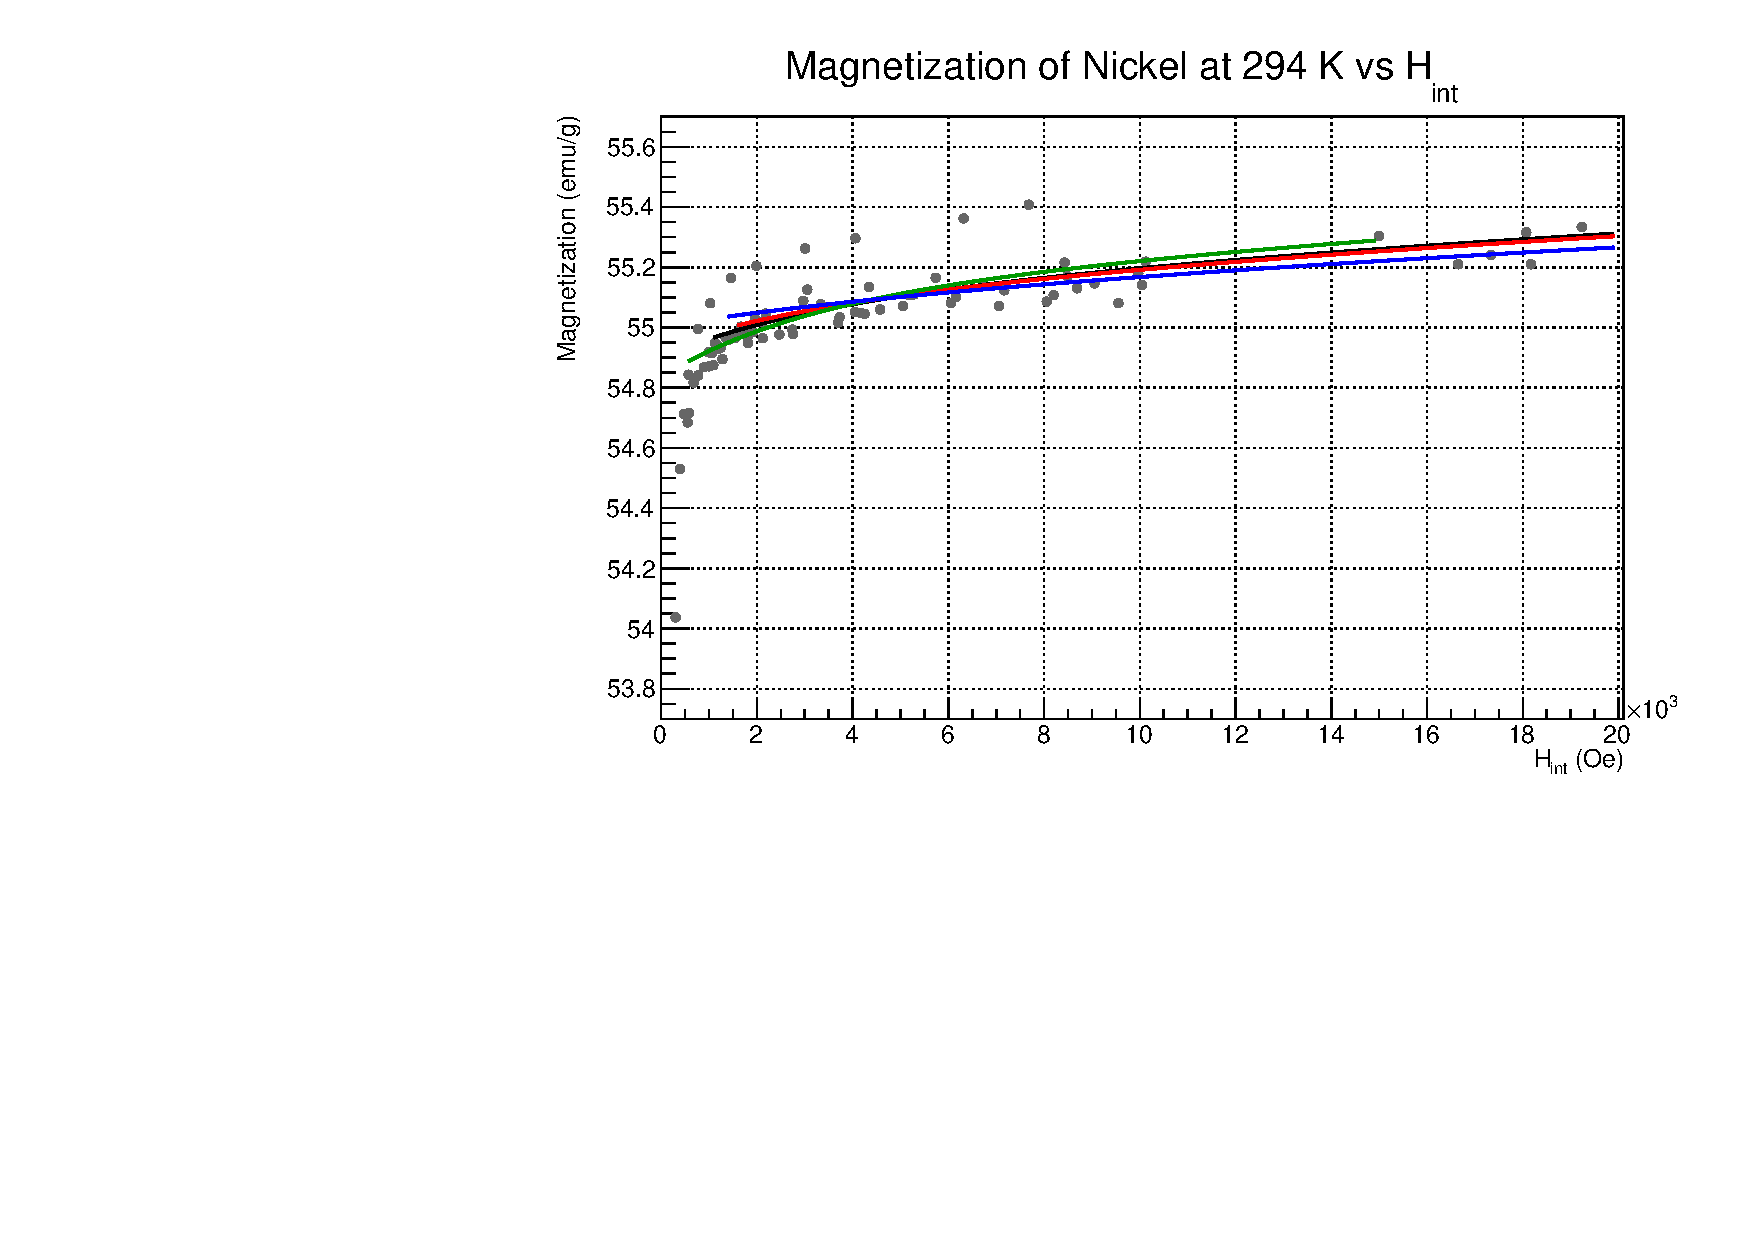
\includegraphics[width=0.7\textwidth]{NiCombinedFit_vs_Hint.pdf}
\caption{Fits to magnetization data using Eq. 10 from \cite{PauthenetMar1982}. The different results demonstrate the systematic uncertainty associated with using this parameterization. The blue line represents a fit over the range 1.3-20 kOe with the saturation magnetization as a single fit parameter. The remaining fits utilize an additional fit parameter allowing the 0 of the ordinate to float but with different ranges of data fit as can be seen in the figure.}
\label{fig:mag_fit_Ni}
\end{figure}
\begin{figure}
\centering
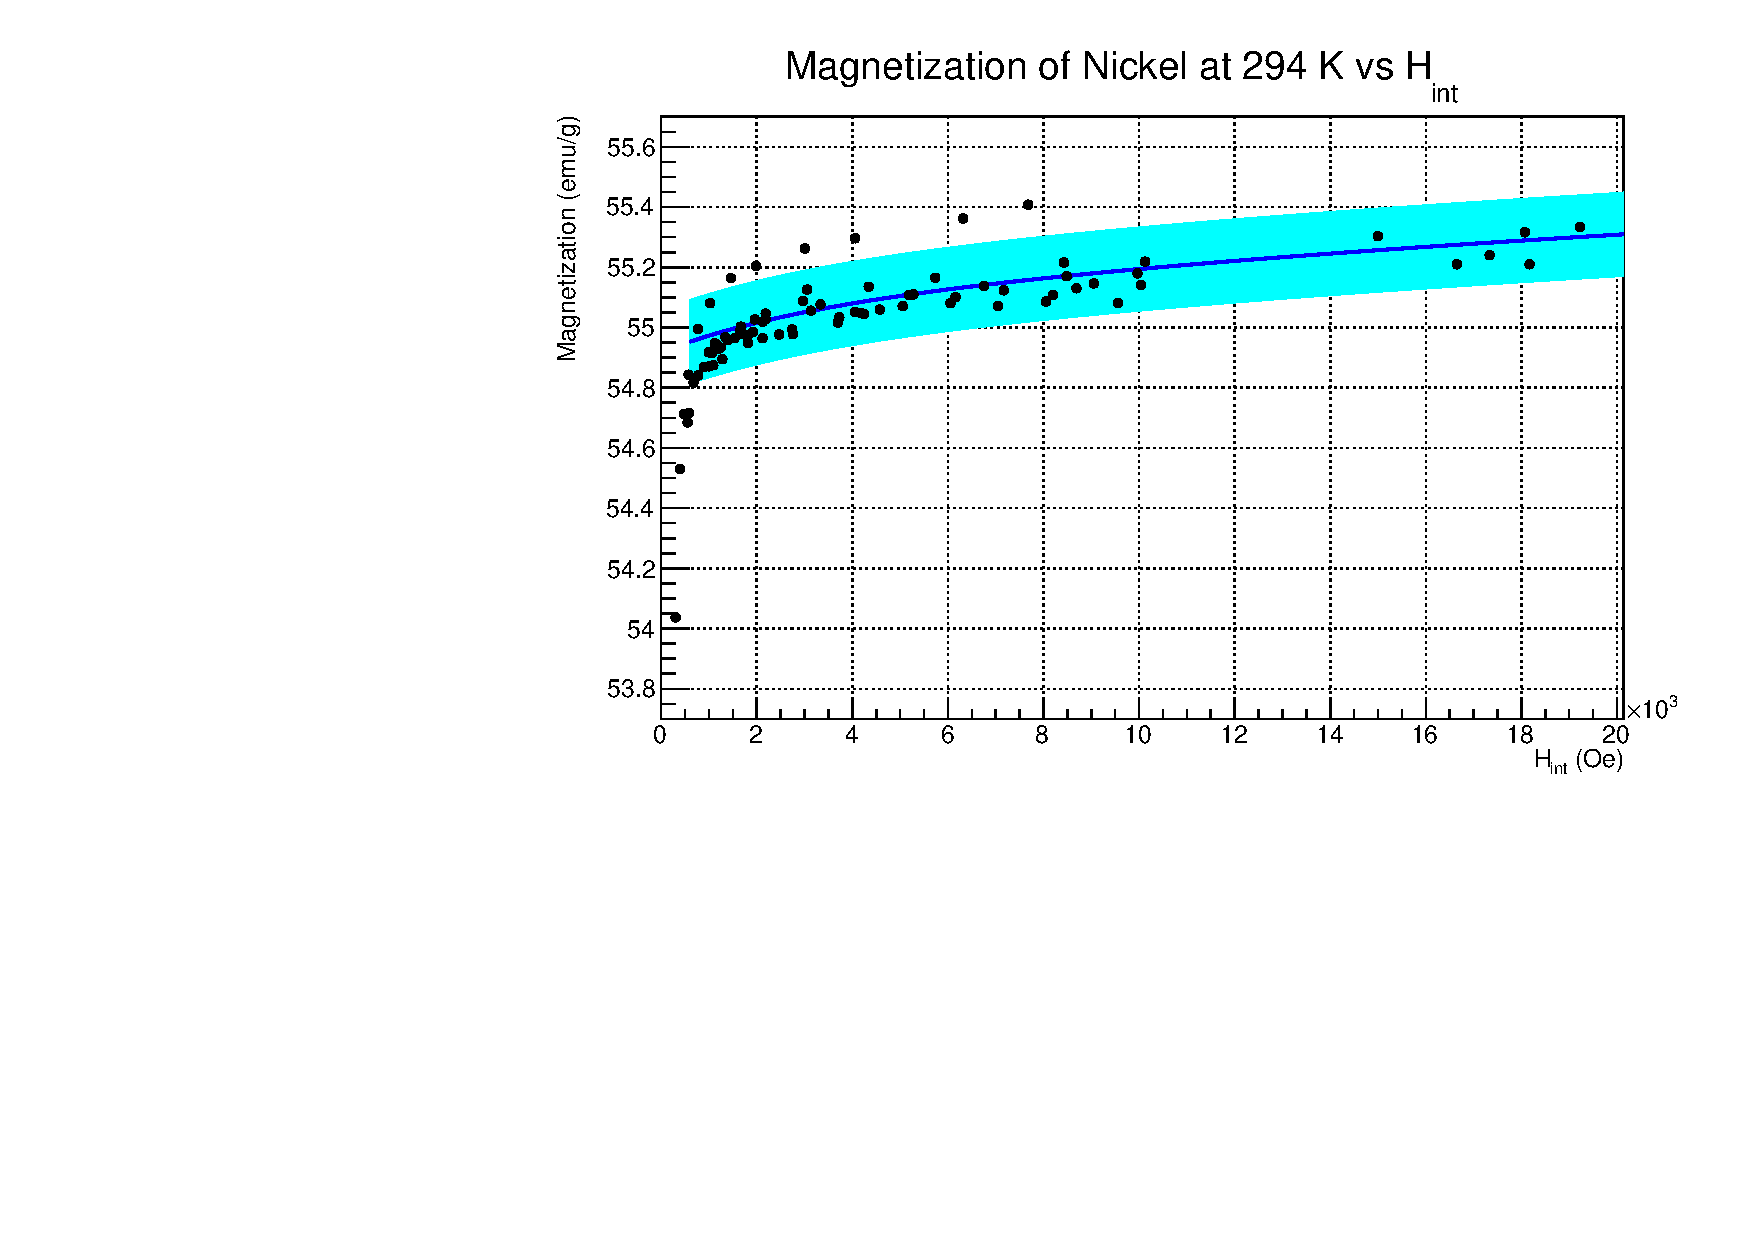
\includegraphics[width=0.7\textwidth]{NiCombinedFitErrorBand_vs_Hint.pdf}
\caption{Published magnetization data from various sources for Ni plotted versus internal field corrected to 294$^{\circ}$K and shown with proposed parametrization curve for internal fields up to 20~kOe (2~T). The curve is approximately the average of the two central curves in Fig. \ref{fig:mag_fit_Ni}. For a thin nickel foil magnetized out of plane (normal to the surface) close to saturation, the difference between the internal and applied field is about 0.6~T so 2~T external field corresponds to 1.4~T internal field. The error band corresponds to 0.14 emu/g or $\sim$0.25\%. }
\label{fig:mag_errorband_Ni}
\end{figure}
\FloatBarrier
\subsubsection{Magnetocrystalline anisotropy and Co}
As previously mentioned, the crystal structure of ferromagnetic elements  creates axes along which it is easier or harder to magnetize the material. The origin of this anisoptropy is nicely explained by a quote from {\it An Introduction to Magnetic Materials} by Cullity and Graham \cite{Cullity2008}:

\begin{quote}
Crystal anisotropy is due mainly to spin-orbit coupling. By coupling is meant a kind of interaction. Thus we can speak of the exchange interaction between two neighboring spins as a spin-spin coupling. This coupling can be very strong, and acts to keep neighboring spins parallel or antiparallel to one another. But the associated exchange energy is isotropic; it depends only on the angle between adjacent spins, as stated by Equation 4.29, and not at all on the direction of the spin axis relative to the crystal lattice. The spin-spin coupling therefore cannot contribute to the crystal anisotropy.


The orbit-lattice coupling is also strong. This follows from the fact that orbital magnetic moments are almost entirely quenched, as discussed in Section 3.7. This means, in effect, that the orientations of the orbits are fixed very strongly to the lattice, because even large fields cannot change them.


There is also a coupling between the spin and the orbital motion of each electron. When an external field tries to reorient the spin of an electron, the orbit of that electron also tends to be reoriented. But the orbit is strongly coupled to the lattice and therefore resists the attempt to rotate the spin axis. The energy required to rotate the spin system of a domain away from the easy direction, which we call the anisotropy energy, is just the energy required to overcome the spin-orbit coupling. This coupling is relatively weak, because fields of a few hundred oersteds or a few tens of kilamps per meter are usually strong enough to rotate the spins. Inasmuch as the ��lattice�� consists of a number of atomic nuclei arranged in space, each with its surrounding cloud of orbital electrons, we can also speak of a spin-lattice coupling and conclude that it too is weak.

\end{quote}

Iron and nickel (iron is body-centered cubic and nickel is face-centered cubic) have hard, medium and easy magnetization axes due to their crystal lattice structure. Magnetization along any axis other than the easy axis requires a larger applied magnetic field due to the anisotropy energy. The plots in Fig. \ref{fig:anisotropy_Ni_Fe} show the magnetization curves for iron and nickel along each of their magnetocrystalline axes. It is interesting that each of the magnetization curves in Fig \ref{fig:anisotropy_Ni_Fe} appears to approach the same saturation magnetization. Pauthenet measures the saturation magnetization with precision along the different crystallographic axes for Ni and Fe and concludes that the saturation magnetization is the same \cite{PauthenetNov1982}. 
\begin{figure}[ht]
\centering
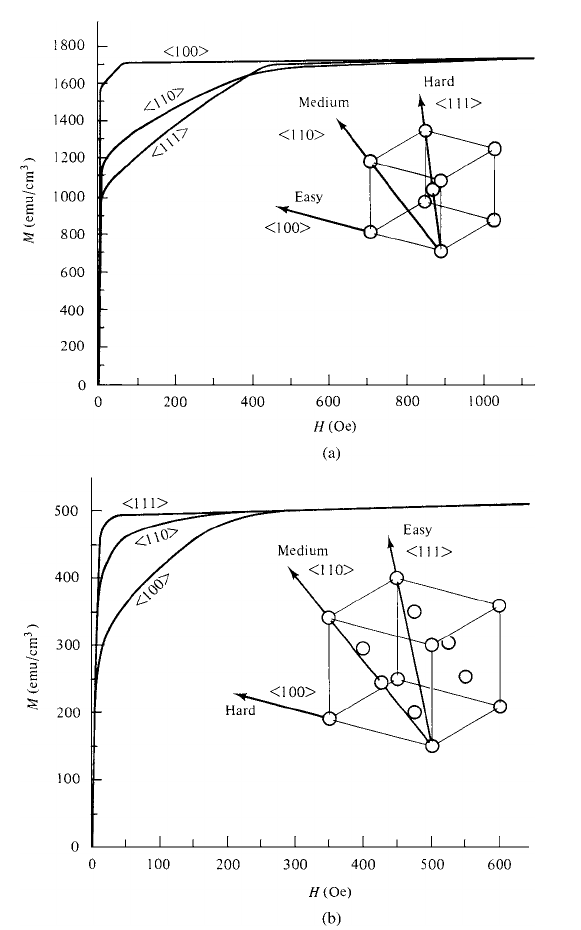
\includegraphics[width=0.5\textwidth]{anisotropy_Ni_Fe.png}
\caption{Magnetization curves for single crystals of Fe (a) and Ni (b) demonstrating the relative difficulty of magnetizing the crystals along different directions. (Figure taken from \cite{Cullity2008}.)}
\label{fig:anisotropy_Ni_Fe}
\end{figure}

The crystal structure of cobalt (close-packed hexagonal at room temperature) creates a greater magnetocrystalline anisotropy than it does for the other two ferromagnetic elements. Cobalt has an easy axis of magnetization and a hard axis perpendicular to the easy axis as can be seen in Fig. \ref{fig:anisotropy_Co} taken from \cite{Cullity2008}. What is striking about these magnetization curves is how difficult it is to magnetize cobalt along its hard axes. A feature not apparent from the $\sim$1~T applied field in Fig. \ref{fig:anisotropy_Co} is that the saturation magnetization is different along the easy and hard axes. Pauthenet measured this difference to be at the 0.5\% level in his careful study of magnetization versus field\cite{PauthenetNov1982}. In a polycrystalline sample such as a foil that might be utilized in the M\o ller polarimeter, it is not apparent how to determine the saturation magnetization. Perhaps it is close enough to average the magnetization curves with twice the weighting on the hard axis value to account for the two orthogonal axes perpendicular to the single easy axis. It is also not apparent how high a field would be required to saturate a cobalt foil normal to its surface.

I have not found an explanation for the magnetization anisotropy in cobalt, but I wonder if the difference is primarily due to the contribution from the orbital magnetization. It is easy to imagine that with significantly different anisotropy constants along the various crystal axes that the sensitivity of the orbital motion to the applied field might be direction-dependent as well. This explanation would also involve a direction dependence to the ratio of magnetization from electron spin to that of the total spin further complicating the interpretation of results using a cobalt foil. 

At temperatures above $690^{\circ}$K the crystal structure of Co becomes face-centered cubic, whereas below that it transitions to close-packed hexagonal. According to Owen {\it et. al}, the crystal structure of polycrystalline cobalt will typically be a mixture of face-centered and close-packed hexagonal crystals\cite{Owen1954}. In any case, given the uncertainties for determining the magnetization for cobalt, its value as a target foil is greatly diminished below the 1\% level.  Quoting from Myers and Sucksmith \cite{Myers1951}
\begin{quote}
On account of the large magnetic anisotropy of hexagonal cobalt and the random orientation of the crystal grains, no reliable values of saturation magnetization can be obtained from the measurements on polycrystalline cobalt at and below room temperature, the magnetic anisotropy becoming more pronounced at lower temperatures. Furthermore, it has been shown be many workers, in particular, Edwards \& Lipson (1943) and Toiano \& Tokich (1948), that polycrystalline cobalt at room temperature is often of mixed-phase content possessing close-packed hexagonal and face-centered cubic structures both being present. Hence apart from the difficulty of magnetization of cobalt, the fact that the two phases of cobalt may co-exist make the significance of some of the results obtained by Wiess \& Forrer (1929) and by Allen \& Constant (1933) very uncertain.
\end{quote}
The reasons for not using cobalt target foils are summarized below.
\begin{itemize}
\item{Large systematic error on magnetization. The best data I could find for the magnetization of cobalt was taken by Pauthenet (see Fig. 3 in \cite{PauthenetMar1982}), for which he quotes a systematic error of 0.5\%.}
\item{Magnetic anisotropy. The magnetic anisotropy of cobalt creates a magnetization that is axis dependent with magnetization values along the hard and easy axes that are different at the  0.5\% level. It is not clear how to choose the value for polycrystalline cobalt.}
\item{Crystal structure uncertainty. The crystal structure of cobalt may vary from sample to sample and may depend on the annealing process or history of heating/cooling. This will create differences in saturation magnetization from sample to sample.}
\item{Source of anisotropy. It is not known if the anisotropy in saturation magnetization is caused primarily by the orbital or spin which adds an additional uncertainty in determining the fraction of magnetization from the spin.}  
\end{itemize}

\begin{figure}[ht]
\centering
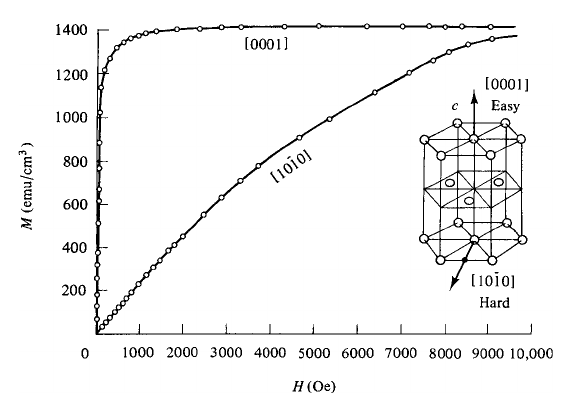
\includegraphics[width=0.5\textwidth]{anisotropy_Co.png}
\caption{Magnetization curves Co demonstrating the relative difficulty of magnetizing the crystal along different directions. (Figure taken from \cite{Cullity2008}.)}
\label{fig:anisotropy_Co}
\end{figure}
\FloatBarrier
\subsubsection{\label{sec:target_heating}Target heating and temperature corrections}
\begin{wrapfigure}{r}{0.3\textwidth}
\vspace{-20pt}
\centering
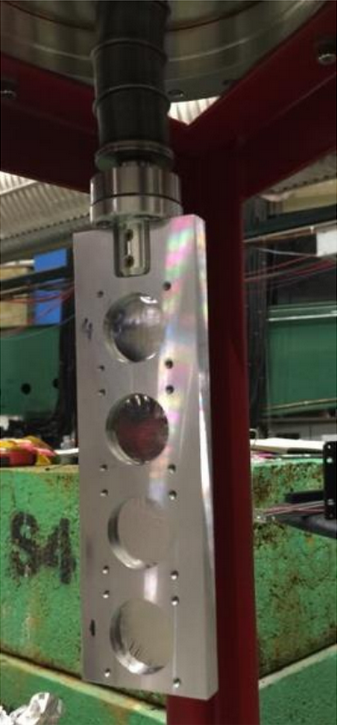
\includegraphics[width=0.25\textwidth]{target_ladder.png}
\caption{Target ladder with four thin iron foil disks. The support structure is aluminum.}
\label{fig:target_ladder}
\end{wrapfigure}
When the electron beam is on target during a M\o ller polarimetry measurement, the foil heats up a few tens of degrees. Since there is a slight temperature dependence to the magnetization a correction will have to be applied. The further from the Curie temperature of the material, the smaller the correction will be. Therefore, we can expect the beam heating correction for Ni to be higher than that of Fe. In the absence of a direct way of determining the temperature of the foil at the beam spot during operation or of monitoring the relative magnetization {\it in situ}, an estimate of the temperature increase must be made. This section provides a calculation of the foil heating from the electron beam under a set of assumptions.

The thin foil disks used in the M\o ller polarimeter are a few microns thick and about 1 inch in diameter (see Fig. \ref{fig:target_ladder}). The electron beam is approximately centered on the target disk during operation to avoid scattering off the aluminum ladder. The electron beam is approximately Gaussian with a 1~$\sigma$ diameter of 90$~\mu$m give or take a few tens of microns. The beam is not typically rastered on the M\o ller target but has a natural helicity-correlated jitter of a few tens of microns. Silviu Covrig from Jefferson Lab kindly provided an analysis using computational fluid dynamics under the following assumptions:
\begin{itemize}
\item{The beam introduces a heat load that is Gaussian on a circle with a 1-$\sigma$ diameter of 90~$\mu$m centered on the foil disk.}
\item{Radiative black-body cooling is negligible.}
\item{The aluminum frame constitutes an approximately infinite heat sink i.e. the temperature of the aluminum frame remains at or near room temperature.}
\item{The foils are 1 inch in diameter and in perfect thermal contact with the aluminum frame.}
\end{itemize}

The temperature distribution of for a 10~$\mu$m thick Fe foil under a 2~$\mu$A heat load provided by Silviu using CFD can be seen in Fig. \ref{fig:target_heating}. The red shows the distribution of heat across the foil all the way to the edge where it is assumed to be held at 300~K, the assumed temperature of the aluminum frame in this calculation. The black tip of the distribution is the part of the foil inside the 90~$\mu$m beam envelope. The temperature-dependent thermal conductivity for Fe was taken from a materials database. The maximum temperature increase at the center of the foil is 40$^{\circ}$C. A similar computation was performed for Ni assuming a simpler constant thermal conductivity and found a nearly identical distribution with a maximum temperature differential of 39.5$^{\circ}$C also for a 2~$\mu$A beam load. This model also shows that for foil thickness in our range of interest, the heating is independent of foil thickness. The maximum temperature differentials are the same for 10~$\mu$m and 20~$\mu$m foils for beam currents from 1-4~$\mu$A. Furthermore, this model also shows that temperature rise is nearly linear in beam current with the following data provided for the Fe foil: 
\[
\Delta \textrm{T}_{max}(1~\mu\textrm{A})=19.74^{\circ}\textrm{C},~~~~\Delta \textrm{T}_{max}(2~\mu\textrm{A})=40.08^{\circ}\textrm{C}~~~~\Delta \textrm{T}_{max}(4~\mu\textrm{A})=82.58^{\circ}\textrm{C}.
\]

Assuming the average temperature rise is about 1$^{\circ}$C below the maximum gives a 19.5$^{\circ}\textrm{C}/\mu$A for both Ni and Fe. Conservatively estimating the temperature differential calculation to be accurate at the 15\% level gives $\delta\textrm{T}=19\pm3~(^{\circ}\textrm{C}/\mu\textrm{A})$.

\begin{figure}[h]
\centering
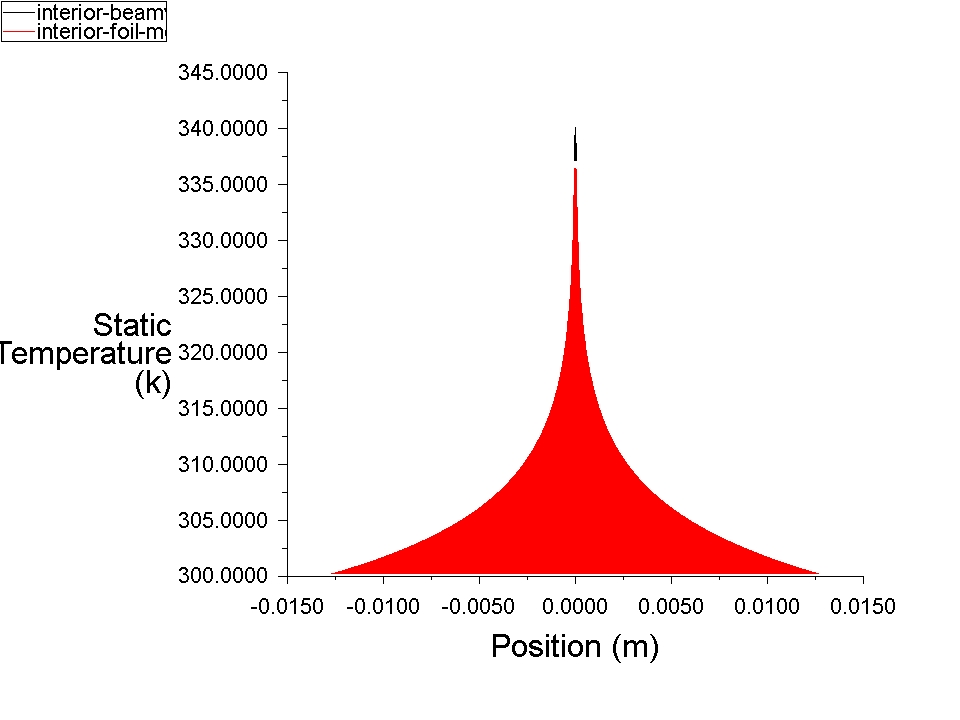
\includegraphics[width=0.7\textwidth]{target_heating_Fe.jpg}
\caption{CFD calculation of the heat distribution in a 1~inch diameter, 10~$\mu$m thick Fe foil under a 2~$\mu$A beam load. The electron beam is assumed to have a Gaussian distribution with a 90~$\mu$m 1-$\sigma$ diameter. The black tip of the distribution is the part of the foil inside the 90~$\mu$m beam spot. The maximum temperature is 340~K or 40 degrees above the temperature of the aluminum frame assumed to be 300~K.}
\label{fig:target_heating}
\end{figure}

Using the model of the temperature dependence of magnetization for iron and nickel from \cite{PauthenetMar1982,PauthenetNov1982} yields the correction shown in Fig. \ref{fig:temperature_correction}. The model was evaluated for applied fields of 2~T for nickel and 4~T for iron. A linear fit to the region of interest for heating from an electron beam between 1 and 2~$\mu$A yields slopes of -0.027~(emu g$^{-1}$$^{\circ}$C$^{-1}$) for Ni and  -0.024~(emu g$^{-1}$$^{\circ}$C$^{-1}$) for Fe. Thus an uncertainty of $\pm$3~$^{\circ}$C/$\mu$A gives an uncertainty in the magnetization for both Fe and Ni of $\pm0.08$~(emu~g$^{-1}~\mu$A$^{-1}$).
\begin{figure}[ht]
\centering
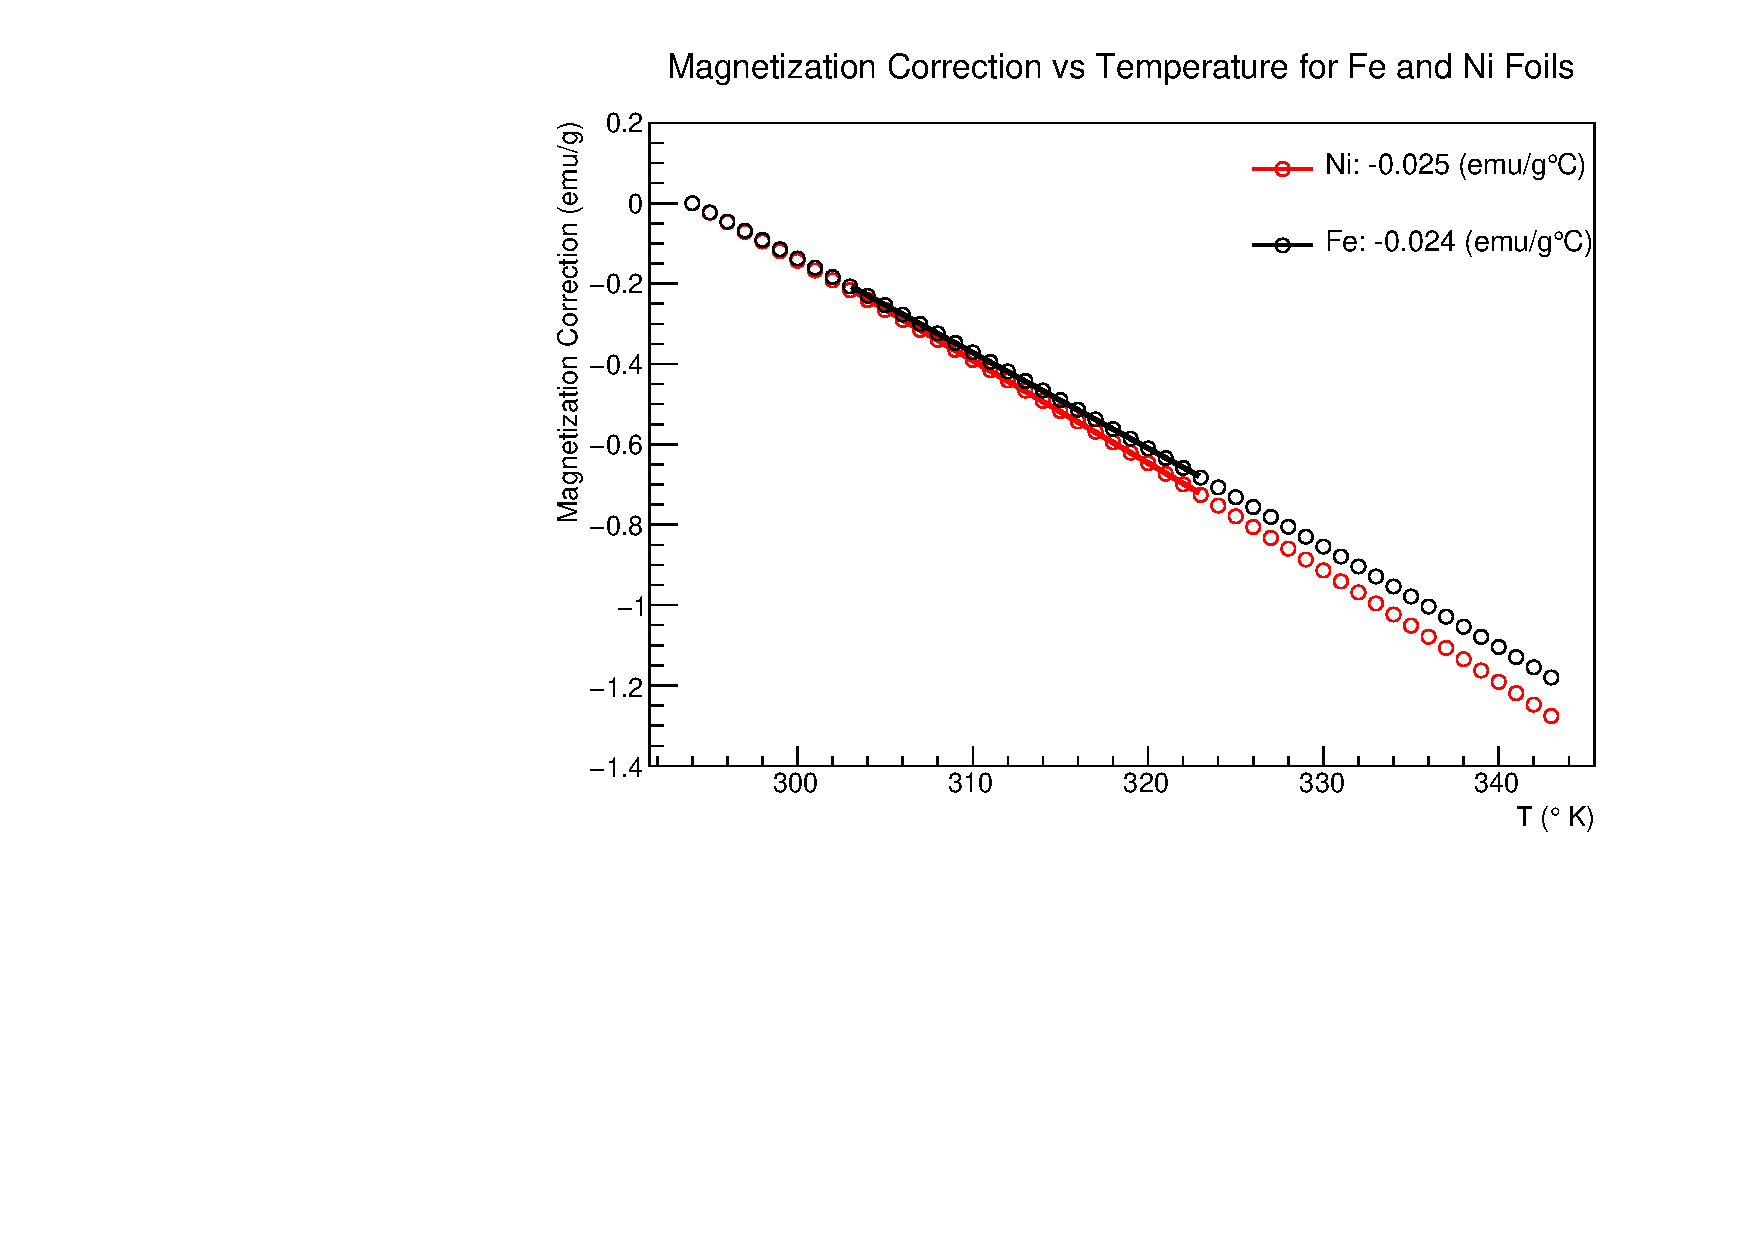
\includegraphics[width=0.7\textwidth]{target_heating_correction.pdf}
\caption{Temperature correction as a function of temperature above room temperature (assumed to be 294 K) for nickel and iron using the model in \cite{PauthenetMar1982,PauthenetNov1982}. The model was evaluated for applied fields of 2~T for nickel and 4~T for iron. The fits are over the temperature range 310 to 338 $^{\circ}$K covering the range plus uncertainty for a beam of 1 to 2~$\mu$A.}
\label{fig:temperature_correction}
\end{figure}
%\begin{figure}[h]
%\centering
%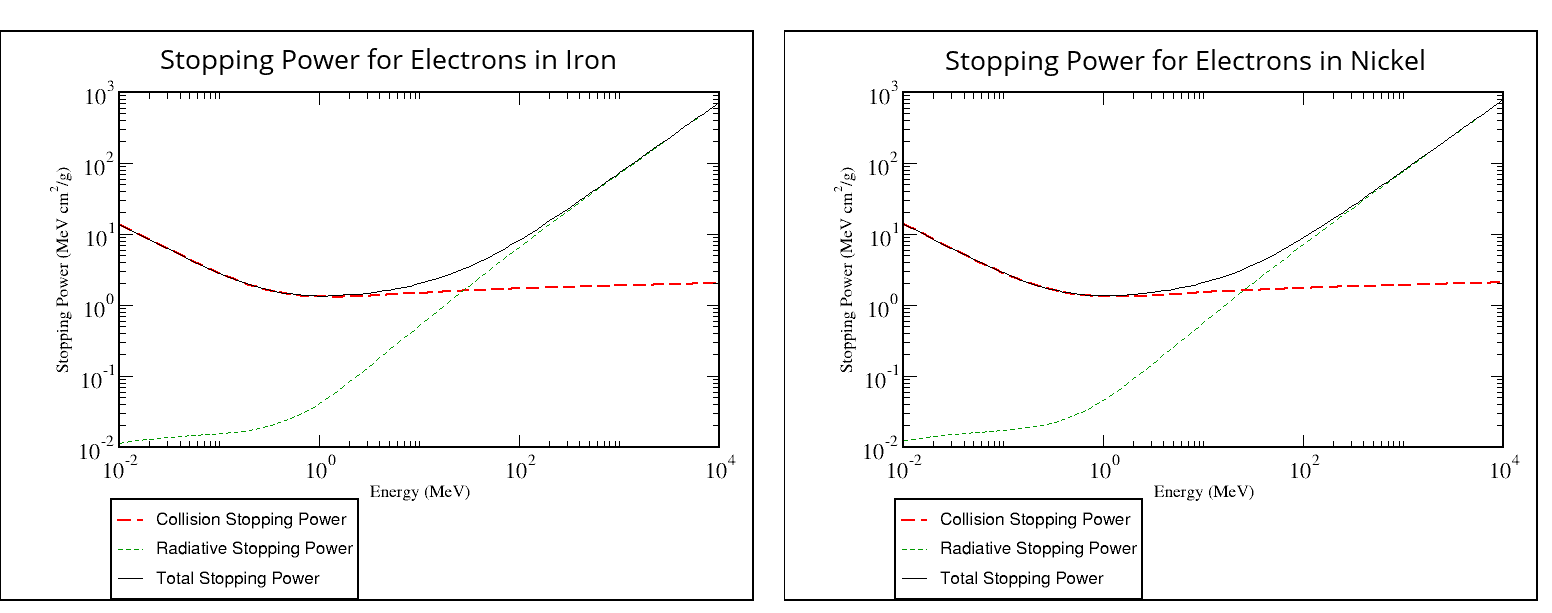
\includegraphics[width=0.9\textwidth]{FeNi_stopping_power.png}
%\caption{Electron stopping power in iron and nickel as a function of electron energy (source PDG https://physics.nist.gov/cgi-bin/Star/e\_table.pl).}
%\label{fig:FeNi_stopping_power}
%\end{figure}
%A simple form of the heat equation in cylindrical coordinates is given by
%\begin{equation}
%\rho C_p\frac{\partial T}{\partial t}=\frac{1}{r}\frac{\partial}{\partial r}\left(kr\frac{\partial T}{\partial r}\right)+\frac{1}{r^2}\frac{\partial}{\partial \phi}\left(k\frac{\partial T}{\partial \phi}\right)+\frac{\partial}{\partial z}\left(k\frac{\partial T}{\partial z}\right)+g(r,\phi,z),
%\label{eq:heat}
%\end{equation} 
%where $\rho$ is the density of the material, $C_p$ is the specific heat capacity, $k$ is the conductivity and $g(r,\phi,z)$ is the heat power generated per unit volume in the material as a function of position. If we think of the steady state where $\frac{\partial T}{\partial t}=0$ and where we assume that there is only a radial dependence to the temperature, and with conductivity $k$ a constant, Eq. \ref{eq:heat} simplifies to
%\begin{equation}
%\frac{1}{r}\frac{\partial}{\partial r}\left(r\frac{\partial T}{\partial r}\right)+\frac{g(r)}{k}=0.
%\label{eq:heat_simp}
%\end{equation} 

%Approximating the electron beam as having a 2-D Gaussian current profile with width $\sigma=90~\mu$m, the heat generation per unit volume can be written as 
%\begin{equation}
%g(r)=\frac{I_0S\rho}{2\pi\sigma^2}e^{-r^2/2\sigma^2},
%\label{eq:specific_heat_gen}
%\end{equation}
% where $I_0$ is the beam current in amperes and $S=2.0\left(\frac{\textrm{MeV~cm}^2}{\textrm{g}}\right)=3.2\times10^{-13}\left(\frac{\textrm{J~cm}^2}{\textrm{g}}\right)$ is the stopping power for electrons in Fe and Ni. Integrating once gives
 
%\begin{equation}
%k2\pi r\frac{\partial T}{\partial r}=\frac{I_0S\rho}{\sigma^2} e^{-r^2/2\sigma^2}+\textrm{const}.
%\end{equation}
%Since the total heat energy is passing through the circumference ($r=R$), then we can say $-\left(k2\pi r\frac{\partial T}{\partial r}\right)\rvert_{r=R}=I_0S\rho\delta$, where $\delta$ is the foil thickness. Since the beam spot is small compared with the target size, the first term is $\sim0$ at the edge $\textrm{const}\approx-I_0S\rho\delta$. Integrating from $r=0$ to $r=R$ gives
%\[
%\Delta T = \frac{I_0S\rho}{2\pi k\sigma^2} \int_0^R\frac{e^{-r^2/2\sigma^2}dr}{r}-I_0S\rho\delta\int_0^R\frac{dr}{r}
%\]

\FloatBarrier

\subsubsection{Effect of impurities}
This section looks at the effect of impurities on the measured magnetization. The experiments whose data are used in this analysis (with the possible exception of the measurement at NASA by Behrendt {\it et al.}) utilized highly pure Fe and Ni samples. Table \ref{tab:impurities} lists the level of impurities in the samples used in the various experiments whose data are used in this analysis. Although Weiss and Forrer \cite{Weiss1929} do not give a numerical value for the level of impurities they assure us that there were no impurities at a measurable level. They used this highly pure sample for the most precise results and many samples of less pure iron for less accurate studies. The less pure sample had a total of 0.22\% impurities with 0.09\% of that being carbon. Since hundreds of ppm were easily measured we can be assured that the pure sample was much better than this. Although the NASA measurement by Behrendt {\it et al.} does not list a purity level for the sample, given the reputation and quality of science from this institution combined with the fact that they were verifying past measurements for pure iron, it is difficult to believe they would utilize a sample with $>$0.1\% impurities.  
\begin{table}[htp]
\caption{Level of impurities from the various measurements used in this analysis.}
\begin{center}
\begin{tabular}{|l|c|c|}\hline
Experiment&Element&Impurity Fraction\\\hline
Weiss and Forrer \cite{Weiss1929} & Fe&``No detectable impurities"\\
R. Sanford {\it et al.}(NIST)\cite{Sanford1941} & Fe&$<$0.01\%\\
H. Danan \cite{Danan1959, Danan1968}& Fe&Same as Weiss and Forrer\\
Arajs and Dunmyre \cite{Arajs1964}\cite{Arajs1967}&Fe& $\sim$600~ppm\\
Crangle and Goodman \cite{Crangle1971} & Fe & 0.06\% and 0.006\%\\
Behrendt and Hegland (NASA)\cite{Behrendt1972} & Fe & Not given\\\hline
H. Danan \cite{Danan1959, Danan1968} & Ni&0.01\% \\
Arajs and Dunmyre \cite{Arajs1963, Arajs1965, Arajs1967}&Ni& $\sim$30~ppm\\
Crangle and Goodman \cite{Crangle1971} & Ni & 0.05\% and 0.005\%\\
R. Shull {\it et al.}(NIST) & Ni & 10~ppm\\\hline
\end{tabular}
\end{center}
\label{tab:impurities}
\end{table}%
Generally speaking, addition of non-ferromagnetic impurities decreases the magnetization (see for example \cite{Luborsky1980, Ahern1958, Sanford1941}). Sanford {\it et al.} corrected for the effect of $\sim0.01\%$ impurities which yielded a correction at the $\sim0.02\%$ level\cite{Sanford1941}. Ahern {\it et al.} also found that adding copper to nickel reduced the magnetization by about 2\% for every 1\% of the nickel replaced by copper. Using the assumption of magnetization being reduced by about 2\% for every 1\% of impurities to set the scale for our uncertainty, we see that the largest error (0.12\%) would be in the Arajs and Dunmyre data on iron. Given the purity of the data samples and the systematic error already assigned from the spread in the data, I believe it is safe to assume that the error from impurities in the determination of magnetization for Fe and Ni is negligible. We will have to revisit impurities once again in the determination of the spin component of the magnetization.

Another source of impurities generally not accounted for in assays is the surface oxidation. Iron oxides such as Fe$_3$O$_4$, have a much smaller magnetization than pure Fe. The research group of Alex Gray, a physicist at Temple University who does XMCD measurements of materials at the Advanced Light Source, took an Fe foil provide to our group by Jefferson Lab and measured its magnetic properties. This measurement only probed the first few nanometers of the foil, but there was evidence of oxides on the surface although it looked shiny and clean. In private communication, Alex confirmed that it is usual to have a couple of nanometers of oxidation on the surface of Fe samples that were not properly cleaned. This suggests that foils nearing micron level thickness will have surface contamination from oxides at the 0.1\% level. To make this uncertainty negligible I recommend using foils 10~$\mu$m or thicker. This, of course, does not include a more difficult to quantify level of oxidation inside the foil resulting from the method in which it is manufactured (eg. rolled or pressed).

\subsubsection{Nuclear contribution to the magnetic moment}
Discussion of the nuclear contribution to the magnetic moment appears to be absent from the literature on magnetization measurements. This is most likely due to the suppression of the nuclear magneton relative to the Bohr magneton by the electron to proton mass ratio ($\mu_B/\mu_N=m_e/m_p$), a factor of about 1/2000. However, in the determination of target polarization for the M\o ller polarimeter, effects at the 0.1\% level require consideration. In the nucleus spins are paired in such a way that all even-even nuclei have zero spin. Fortunately for us, the isotopic distribution of iron (26 protons) is such that 97.9\% of natural iron is from even-even isotopes. The single even-odd naturally occuring isotope $^{57}Fe$ has a negligible nuclear spin of 0.09$\mu_N$\cite{Locher1965}. For nickel (28 protons) the situation is also favorable with natural nickel being composed of 98.9\% even-even isotopes. This gives us another two orders of magnitude suppression and renders the nuclear spin contribution completely negligible. However, for cobalt (27 protons), the only stable isotope has a nuclear spin of 4.63~$\mu_N$, potentially creating errors at the 0.2\% level and adding another reason not to use Co foil.   

\subsection{Determination of $g^{\prime}$ and the spin component of magnetization}
The spin component of the magnetization is obtained from experiments measuring what has become known as $g^{\prime}$, the g-factor obtained from magnetomechanical experiments arising from the Einstein-deHaas effect or the Barnett effect\footnote{The Einstein-deHaas effect (rotation by magnetization) is the rotation of a macroscopic body in a magnetic field when the field is reversed. The Barnett effect (magnetization by rotation) is the converse, the production of a magnetic field by rotation of a macroscopic body.}. In general, the $g$-factor is related the to gyromagnetic ratio $\gamma$ of a charged body as 
\begin{equation}
\gamma=g\frac{e}{2mc}=g\frac{\mu_B}{\hbar},
\label{eq:gyro}
\end{equation}
where $\mu_B$ is the Bohr magneton\footnote{In early publications sometimes the gyromagnetic ratio is given as $\rho=L/M$ the ratio of the angular momentum to the magnetic moment where at other times it is defined in the usual way as the reciprocal $\gamma=1/\rho=M/L$.}. The electron has two g-factors which I will call $g_{sp}\approx2$ for its spin motion and $g_{orb}=1$ for its orbital motion. For atoms with angular momentum from orbital motion and spin, $g$ can take on an arbitrary value. This total $g$ for atomic electrons is referred to as $g^{\prime}$ which is a linear combination of $g_{sp}$ and $g_{orb}$.
In publications from the early to middle 1900's, $g_{sp}$ was assumed to be exactly 2 where we now know it to be (up to a sign) the most precisely measured scientific constant $g_{sp}=2.00231930436182(52)$. In most cases, this $0.1\%$ difference is not consequential, but for the level of precision we are trying to reach for M\o ller polarimetry, this is not negligible and care must be taken to track down wherever 2 has been substituted for $g_{sp}$. The relationship of $g^{\prime}$ to the magnetic moment contribution is often given in the literature in the following form \cite{Meyer1961, Smit1959}
\begin{equation}
g^{\prime}=\frac{2(M_{sp}+M_{orb})}{M_{sp}+2M_{orb}}=\frac{2M_{tot}}{M_{tot}+M_{orb}},
\label{eq:gprime_approx}
\end{equation}
where $M_{orb}$, $M_{sp}$ and  $M_{tot}$ are the orbital, spin and total magnetic moments respectively. This expression immediately leads to the expression of orbital and spin contributions to the magnetic moment as \cite{deBever1997}
\begin{equation}
\frac{M_{orb}}{M_{tot}}=\frac{2-g^{\prime}}{g^{\prime}}, ~~\frac{M_{sp}}{M_{tot}}=1-\frac{M_{orb}}{M_{tot}}.
\label{eq:frac_gprime_approx}
\end{equation}
The derivation of Eq. \ref{eq:gprime_approx} was first done by Kittel in 1949 in his paper ``On the gyromagnetic ration and spectroscopic splitting factor of ferromagnetic substances''\cite{Kittel1949}. It is helpful to follow through the derivation carefully to ensure that it is intended as an exact not approximate equality. From the definition of gyromagnetic ratio we have $\gamma=M_{tot}/J$, where $M_{tot}$ is the total magnetic moment of the atom and $J=L+S$ is the total angular momentum of the atom. We can now use the relationships $M_{sp}=g_{sp}\mu_BS/\hbar$ and $M_{orb}=g_{orb}\mu_BS/\hbar$ along with Eq. \ref{eq:gyro} to re-express $\gamma$ in terms of magnetizations as
\begin{equation}
\gamma=g^{\prime}\frac{\mu_B}{\hbar}=\frac{M_{tot}}{\frac{\hbar}{\mu_B}(M_{sp}/g_{sp}+M_{orb}/g_{orb})},
\end{equation}
or simplifying and substituting $g_{orb}=1$
\begin{equation}
g^{\prime}=\frac{M_{tot}}{M_{sp}/g_{sp}+M_{orb}}=g_{sp}\frac{M_{tot}}{M_{sp}+g_{sp}M_{orb},}
\label{eq:gprime_exact}
\end{equation}
from which we recover Eq. \ref{eq:gprime_approx} if we substitute $g_{sp}=2$. Eq. \ref{eq:gprime_exact} is the exact form which should be used in this analysis. Furthermore, the exact form of Eq. \ref{eq:frac_gprime_approx} is the slightly more complicated
\begin{equation}
\frac{M_{orb}}{M_{tot}}=\frac{g_{sp}-g^{\prime}}{g^{\prime}(g_{sp}-1)}.
\label{eq:frac_gprime_exact}
\end{equation}
This decreases the spin contribution to the total magnetization by $~0.11\%$.

\subsubsection{$g^{\prime}$ for Fe}
The most precise measurments of $g^{\prime}$ come from measurements of the gyromagnetic ratio of iron using the Einstein deHaas effect. These magnetomechanical experiments are highly elaborate requiring high precision to observe the tiny effects of interest. The Einstein-deHaas experiments are simple in principle: a sample is suspended from a torsion pendulum along the axis of a magnetic field. Upon reversal of the field a small torque on the sample is measured primarily due to reversal of the valence electron spins. In practice, these experiments are highly technical since the torques on the sample from the Earth's magnetic field are 7-8 orders of magnitude larger than the torques from spin reversal. Elaborate coil setups were utilized to cancel the Earth's field along with any stray magnetic fields in the region and isolation systems incorporated to keep the sample free from interference from outside vibrations. The gyromagnetic ratio was then determined from the ratio of the angular momentum to the magnetic moment. Similarly complex systems were used in the experiments which measured the Barnett effect. In these experiments a relatively large sample was rotated and the change in magnetic flux measured in a system of pickup coils. 

A compilation of $g^{\prime}$ measurements from magnetomechanical experiments is shown in Fig. \ref{fig:gprime_world_data_Fe}. These data were taken from compilations in two papers\footnote{There were two inconsistencies between these references\cite{Scott1962,Meyer1961} which were resolved as follows. Table 1 of \cite{Meyer1961} has Barnett 1941 $\rho e/mc=1.035$ whereas Barnett\cite{Barnett1952} actually had the following 3 values for different Fe samples: 1.032, 1.032 and 1.034. I use the straight average of  $\rho e/mc=1.0327$ or $g^{\prime}= 1.937\pm0.006$ where error is taken from \cite{Scott1962}. There is also a discrepancy on the value for Meyer and Brown 1957 between the two papers in which case, of course, I went with the value given by Meyer himself \cite{Meyer1961} $g^{\prime}=1.929\pm0.008$, where the error was taken from \cite{Scott1962}.} 
 by G. Scott in 1962\cite{Scott1962} and Meyer and Asch in 1961\cite{Meyer1961}. For reference, the data included in these compilations comes from \cite{Barnett1944,Scott1951,Barnett1952,Scott1962}. The final two measurements done by G. Scott are by far the most precise. It is clear that the error bars do not in all cases reflect the actual systematic error. The systematic errors in these experiments are often determined from the repeatability of the results. Known systematic effects are canceled or averaged by varying techniques and the systematic error is assigned from remaining differences or instability in the data arising from sources not accounted for. It would appear that the systematic error in at least some of the values is underestimated. Scott, without stated justification, concludes that his most recent measurement of $g^{\prime}=1.919\pm0.002$ on a prolate ellipsoid sample is the value to use for iron \cite{Scott1960, Scott1962} even though he measured  $g^{\prime}=1.917\pm0.002$ on a cylindrical sample using the same apparatus. It is worth noting that his latest value  $g^{\prime}=1.919$ appears to be the value taken as standard in the literature (see for example \cite{Wohlfarth1980,Bonnenberg1986}). It is far from clear what systematics may be at play here (sample purity, shape, porosity, preparation/annealing process) or which of the measurements closest represents our sample foil. A naive fit using the quoted systematic error bars gives a value $g^{\prime}=1.9208$.
\begin{figure}[h]
\centering
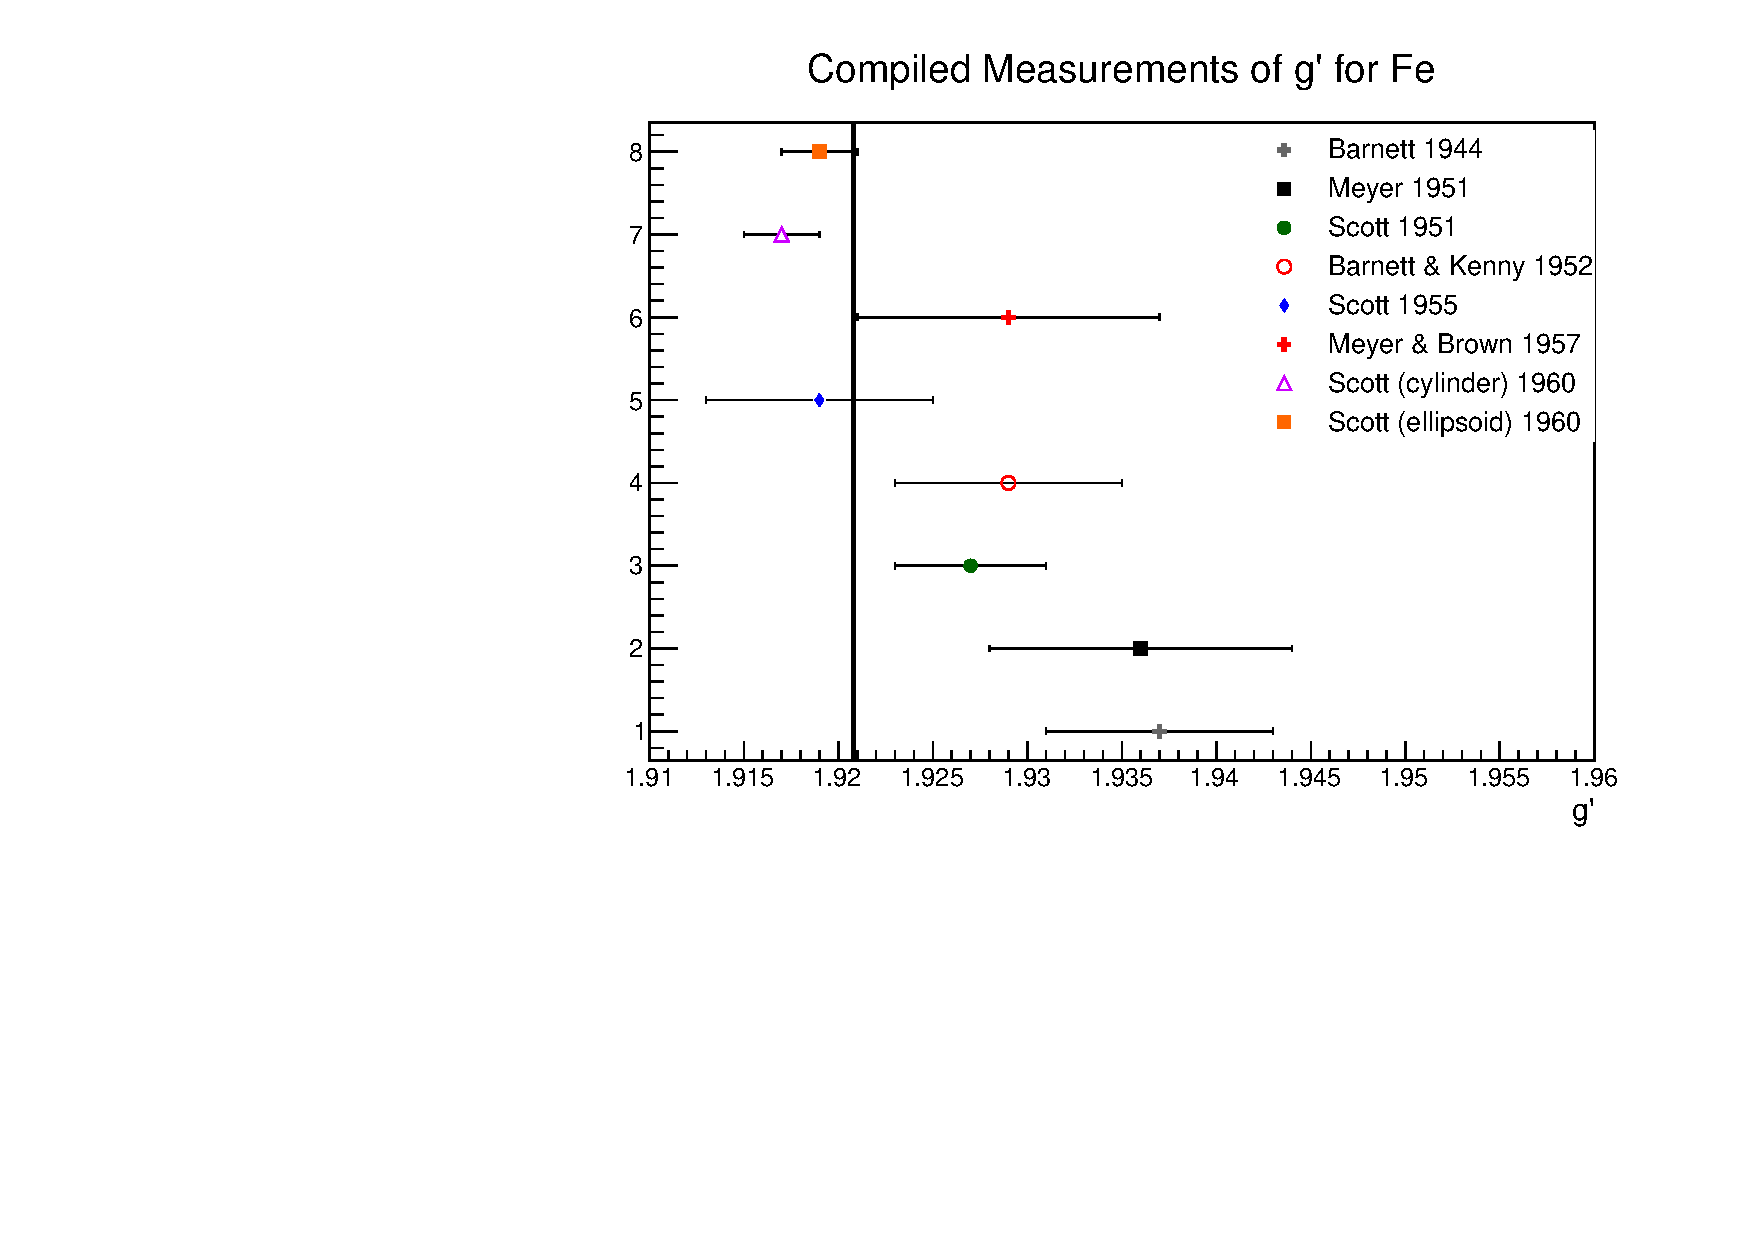
\includegraphics[width=0.8\textwidth]{gprime_world_data_Fe.pdf}
\caption{Values of $g^{\prime}$ for iron as determined by various experiments between 1940 and 1960. The naive constant fit to these data is given by the vertical black line whose value is $g^{\prime}=1.9208$.}
\label{fig:gprime_world_data_Fe}
\end{figure}

For the three samples in used in the measurements $g^{\prime}$ of Fe, the sample purities were as follows: 
\begin{itemize}
\item{Scott cylinder 99.94\% with primary impurities O(0.04\%), C(0.005\%), N(0.004\%), S(0.003\%) and Ni(0.0015\%) \cite{Scott1951}}
\item{Scott ellipsoid, 99.89\% with primary impurities Ni(0.05\%), Si(0.01\%), O(0.005\%), Co(0.005\%) \cite{Scott1960}}
\item{ Meyer 1957, 99.9\% with primary impurities Mn(0.042\%), S(0.029\%), Si(0.02\%) \cite{Meyer1957}}
\item{ Meyer 1958, 99.99\% (negligible impurities) \cite{Meyer1961}}. 
\end{itemize}

Scott carefully measured the effect of mixing the ferromagnetic elements Fe, Co and Ni and since their $g^{\prime}$ values are all within 5\% of each other trace amounts of impurities ($<$1\%) from of Ni and Co in Fe will have negligible effect on the value of  $g^{\prime}$ (see Fig 1 of \cite{Scott1969}). Furthermore, addition of 3\% Si to iron changed the measured g-factor by only 0.5\%. We will see in the coming paragraphs that the spectroscopic g-factor is directly related to $g^{\prime}$ such that if one changes both will. There is little guidance in the literature for the effect of trace amounts of O, Mn, N, C and S on $g^{\prime}$ for Fe. I was also not able to find any way to set the scale for such errors. Perhaps the spread in the measurements of different samples provides a sufficient measure of this uncertainty. 

Related to $g^{\prime}$ is the spectroscopic $g$-factor often referred to as $g$ from ferromagnetic resonance (FMR) experiments\footnote{For a simple explanation of FMR see http://www.physik.fu-berlin.de/einrichtungen/ag/ag-kuch/research/techniques/fmr/index.html}. FMR works by placing a ferromagnetic sample in a resonant microwave cavity. The cavity is placed in a uniform magnetic field at right angles to the direction of propagation of the microwaves. A microwave source feeds the cavity and a detector monitors the energy coming out of the cavity. When the magnetic field is turned on, the magnetic moments of the atoms will begin to precess around the direction of the applied magnetic field with a frequency that depends on the effective magnetic field $H_{eff}$ and the $g$-factor of the sample material material as follows:
\begin{equation}
\hbar\omega=g\mu_BH_{eff}
\label{eq:fmr}
\end{equation}
where $H_{eff}$, the effective magnetic field depends on the applied magnetic field strength as well as the magnetization, shape and relative alignment of the specimen (see \cite{Kittel1949, Smit1959} for a more detailed explanation). The magnetic field strength is then swept over a range until the resonance condition is met where the precession frequency matches that of the microwave cavity. At resonance a drop in power exiting the cavity will be observed due to the energy being absorbed by the sample. Spectroscopic $g$ is determined by measuring the magnetix field which excites this resonance. For a time it was thought that spectroscopic $g$ and $g^{\prime}$ were the same i.e. that spectroscopic and magnetomechanical experiments were measuring the same $g$-factor until Kittel (1949)\cite{Kittel1949} and Van Vleck (1950)\cite{Vleck1950} independently showed that these are distinct although arising from the same physics. In fact, the difference was shown to arise from the contribution of the orbital angular momentum. To a good approximation it can be shown that $g=\frac{2M_{tot}}{M_{tot}-{M_{orb}}}$ where $g^{\prime}$ is given approximately by Eq. \ref{eq:gprime_approx}. Thus, the orbital component increases the magnitude of $g$ and decreases $g^{\prime}$. Using these equations we can easily derive what is known as the Kittel-Van Vleck relationship 
\begin{equation}
\frac{1}{g}+\frac{1}{g^{\prime}}=1.
\label{eq:kittelvanvleck}
\end{equation}
Although this relationship is approximate, it should be good at the 0.1-0.2\% level and it has been shown to work quite well in the literature (see for example Fig. 1 of \cite{Meyer1961}). Therefore, we can utilize spectroscopic measurements of $g$ to check our value of $g^{\prime}$. Figure \ref{fig:gfactor_world_data_Fe} shows a compilation of measurements of $g$ for iron. A naive error-weighted fit to these data gives a value of $g=2.086\pm0.004$. Using Eq. \ref{eq:kittelvanvleck} gives $g^{\prime}=1.9208$ in precise agreement with the error weight fit to $g^{\prime}$ from magnetomechanical experiments. While we cannot place the same confidence in this derived value of  $g^{\prime}$ as the direct measurements, it does provide a greater level of confidence that determinations from completely different techniques appear to be consistent.
\begin{figure}[h]
\centering
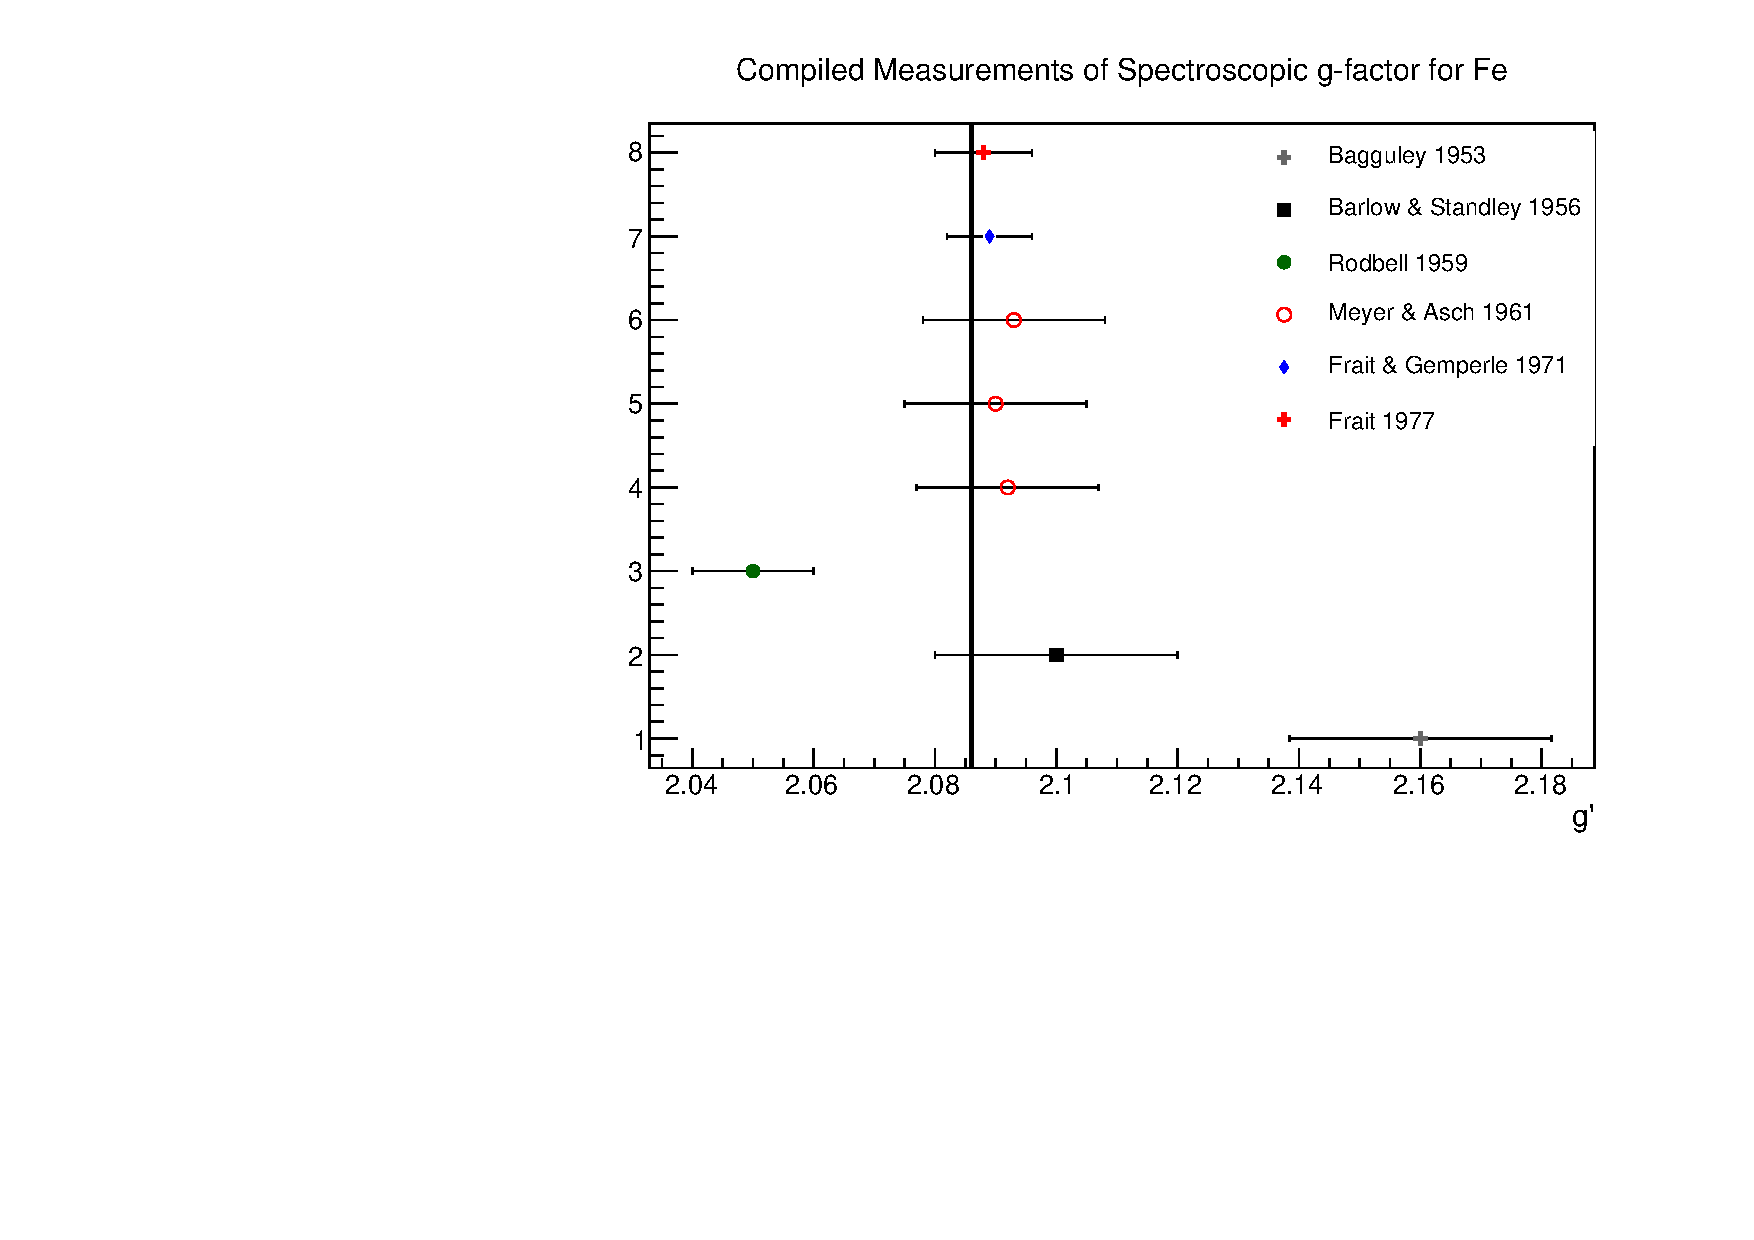
\includegraphics[width=0.8\textwidth]{gfactor_world_data_Fe.pdf}
\caption{Values of spectroscopic $g$ as determined by various experiments over two decades. The error-weighted fit to these data is given by the vertical black line whose value is $g=2.086$.}
\label{fig:gfactor_world_data_Fe}
\end{figure}

{\bf Recommendation for Fe:} In light of these findings my recommendation is that we use the value { $\bf g^{\prime}=1.920\pm0.004$}. The proximity of this number to Scott's $g^{\prime}=1.919\pm0.002$ reflects the fact that after reviewing the world data on $g^{\prime}$ for iron, Scott who made the world's two most precise determinations of this value recommendeded his final value 1.919 as the standard \cite{Scott1962}. Doubling his assigned error reflects unease with the small systematic error given the magnitude of the disagreement with world data.

\subsubsection{ $ g^{\prime}$ for Ni}
A number of measurements of $g^{\prime}$ for nickel were performed by A. J. Meyer {\it et al.}, G. G. Scott {\it et al.} and S. Barnett {\it et al.} during the 1950's. At first there were striking differences in the values found for nickel ranging from 1.83 to $>$1.99. Furthermore, the measurements of spectrocopic $g$ from resonance experiments gave a much lower value of $g^{\prime}$ using the Eq. \ref{eq:kittelvanvleck}. A couple of systematic errors in the measurement techniques of both Meyer and Scott were pointed out by Brown which brought the data into much better agreement\cite{Scott1962}. However, a considerable inconsistency remained between the measurement of Barnett {\it et al.} and that of Scott and Meyer. Barnett determined $g^{\prime}\approx1.91$ compared to the 0.04\% lower $g^{\prime}\approx1.84$ found by Meyer and Scott\cite{Meyer1961,Scott1962}. To investigate the possible reasons for this discrepancy, Meyer measured the Curie temperature and the saturation magnetization of the Ni samples used in each of the measurements. Whereas Scott and Meyer had used nearly pure Ni, Barnett's sample had 1.4\% impurities. The presence of these impurities significantly changed the magnetic properties of his Ni sample such that the Curie temperature was reduced from 360$^{\circ}$C for pure Ni to 285$^{\circ}$C and the saturation magnetization increased from 58.90 to 71.04 (in units of abamp cm$^3$/g)\cite{Scott1962}. Scott concludes that this stark shift in magnetic properties makes Barnett's measurements ``difficult to retain''\cite{Scott1962}. However, this discrepancy provides a scale for the uncertainties arising from impurities in the case of Ni i.e. 1.4\% of impurities shifts the value of $g^{\prime}$ by 3-4\%.

Scott performed a series of four measurements on the same Ni sample in 1952, 1953, 1955 and 1960 and concluded that $g^{\prime}=1.835\pm0.002$\cite{Scott1962}. Meyer {\it et al.} also measured $g^{\prime}$ for different Ni samples in 1957 and 1958 finding 1.852$\pm$0.010 and 1.845$\pm$0.008 \cite{Meyer1961}. An error-weighted fit to these values gives $g^{\prime}=1.836\pm0.002$. However, it is far from clear that this is the correct way to proceed. The impurities in the samples used are as follows:
\begin{itemize}
\item{Scott 99.82\% Ni with main impurities Si(0.1\%), Fe(0.032\%), Mn(0.030\%), and C(0.01\%)\cite{ScottSep1955}}
\item{Meyer 1957 99.9\% Ni with impurities not provided\cite{Meyer1957}}
\item{Meyer 1958 99.99\% with negligible impurities\cite{Meyer1961}}
\end{itemize}

Looking at the impurities in Scott's sample, we can rule out the effects of Fe and Mn as contributing significantly to a systematic offset using the data in \cite{Standley1955, Scott1969}. With carbon impurities at 0.01\% this can be considered negligible. However, I was not able to locate data to rule out the effect of Si impurities at 0.1\% in Ni. Without data to rule out this effect as insignificant, it seems to prudent to add an additional systematic uncertainty to Scott's measurement.

Meyer's analysis of the magnetic properties of the Ni sample used by Scott showed that although the saturation magnetization was changed insignificantly, the Curie temperature decreased by 11$^{\circ}C$. With nearly an $8\times$ improvement in sample purity (1.4\%$\rightarrow$0.18\%) in Scott's sample and an accompanying $8\times$ smaller shift in Curie temperature ($\Delta T_c=75^{\circ}$C$\rightarrow10^{\circ}$C) it is not unreasonable to assume a similar proportional impact on the value of $g^{\prime}$. Barnett measured $g^{\prime}$ higher by $>0.3$\% than Scott and Meyer, so perhaps increasing the uncertainty of Scott's measurement to $\sim$0.3\% or from 0.002 to 0.006 absolute is not unreasonable. One of Barnett's samples also had 0.1\% of impurities; however, its magnetic properties (Curie temperature and saturation magnetization) were unaltered by these impurities and its assigned error (0.01) is already so large that adding uncertainty for this has little effect. The data from Scott and Meyer is shown in Fig. \ref{fig:gprime_world_data_Ni} along with the both the error assigned by Scott to his value and the proposed systematic error. The error-weighted fit to the data using Scott's error is $g^{\prime}=1.836\pm0.002$ with $\chi^2/NDF=4.07/2$. The same fit using my proposed error yields the vertical line shown in Fig. \ref{fig:gprime_world_data_Ni}: $g^{\prime}=1.8411\pm0.0044$ with $\chi ^2/NDF=2.46/2$.

\begin{figure}[h]
\centering
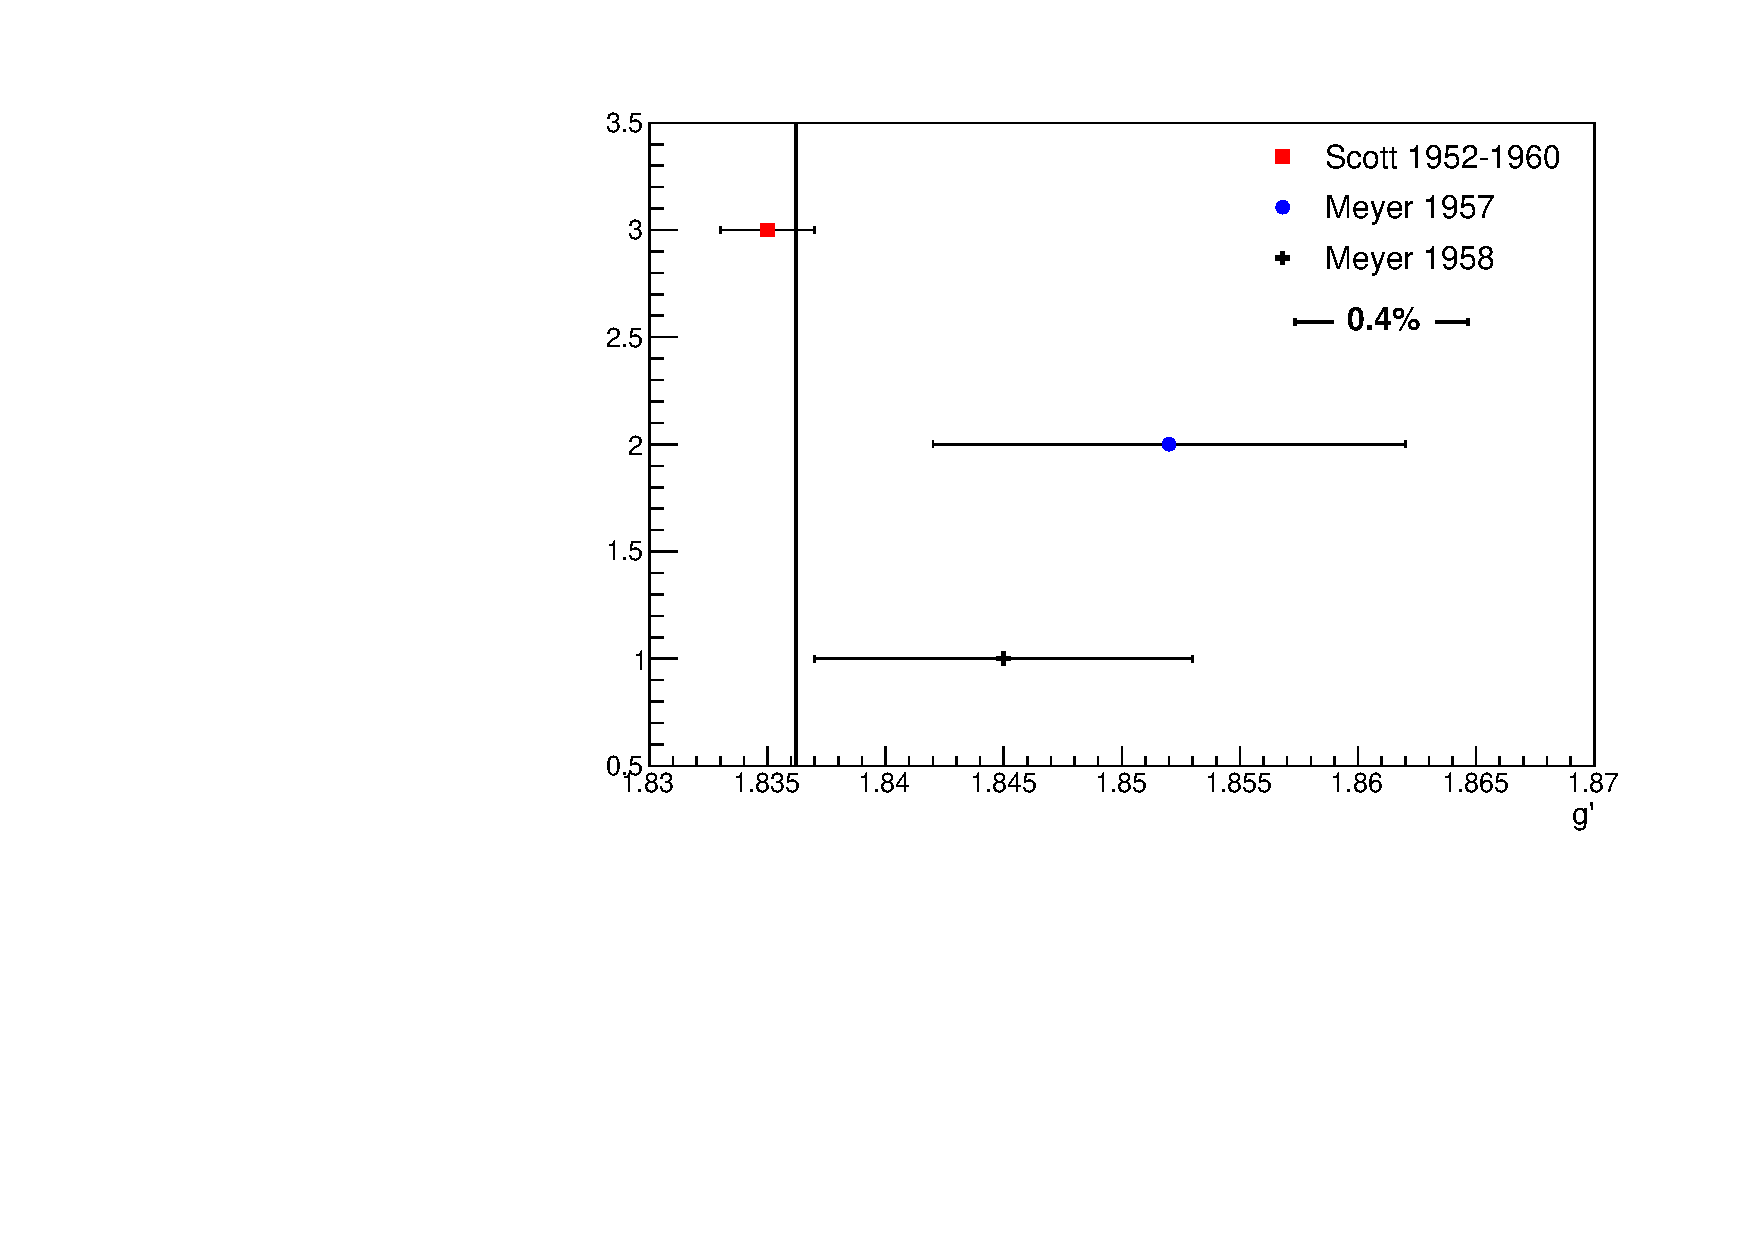
\includegraphics[width=0.8\textwidth]{gprime_world_data_Ni.pdf}
\caption{Values of $g^{\prime}$ for nickel as determined by various experiments between 1950 and 1960. The systematic error on Scott's value as proposed in the text is shown. The error-weighted fit to these data using the proposed error given by the vertical line is $g^{\prime}=1.8411\pm0.0043$.}
\label{fig:gprime_world_data_Ni}
\end{figure}

Once again we can use measurements of the spectroscopic $g$-factor from magnetic resonance experiments and Eq. \ref{eq:kittelvanvleck} as an independent check of our proposed value of $g^{\prime}$. Table II. of Meyer and Asch \cite{Meyer1961} provided a compilation of $g$-factors measured in magnetic resonance experiments and concluded that for nickel $g=2.185\pm0.010$ which translates into $g^{\prime}=1.844\pm0.008$ in good agreement with our proposed value.

{\bf Recommendation for Ni:} In light of these findings my recommendation is that we use the value { $\bf g^{\prime}=1.841\pm0.005$} for nickel. The value comes from an error-weighted fit to Scott's and Meyer's measured values after increasing Scott's systematic error to $\pm0.006$ due to uncertainties from impurities. The error from the fit was 0.0043 which is conservatively rounded up to 0.005.

\subsubsection{\label{sec:gp_temp_dep}Temperature dependence of $g^{\prime}$}
The measurements of $g^{\prime}$ used in this analysis have all been at room temperature which is not well-defined but is broadly accepted to be near 20$^{\circ}$C give or take a few degrees. Although the target foils in the M\o ller polarimeter will generally be at room temperature, during measurements with a typical 1-2~$\mu$A of beam on target, the foils will heat up by 20 to 40 degrees Celsius as we saw in Section \ref{sec:target_heating}. This raises the question of whether or not the room temperature values of $g^{\prime}$ are sufficiently accurate during elevated temperatures.

In Kittel's 1949 paper on the relation of $g$ and $g^{\prime}$, he talks about the temperature dependence of $g^{\prime}$ and suggests there is not enough data to make conclusions\cite{Kittel1949}. Since then several measurements have been made of $g$ across a broad temperature range for the ferromagnetic elements and alloys. These experiments, which measure $g$ since it is a technically much easier measurement than $g^{\prime}$, particularly with changing temperatures, are typically at the 1-2\% precision level. However, a change in $g$ indicates the inverse change in the  $g^{\prime}$ by Eq. \ref{eq:kittelvanvleck}. A nice summary of these measurements is found in \cite{borovik1988}.

It is worth noting that in all cases where pure Ni and Fe were measured, the $g$-factor was always found to be constant within experimental errors, typically at the 1-2\% level. However, for alloys, this is not always the case with variations of several percent being observed (see for example \cite{Gadsden1978, Shanina1998}).

In two cases extremely accurate measurements were made across a broad temperature range, one for pure Ni and the other for 97\% Fe. The first of these was by G. Dewar {\it et al.} in 1977 on pure nickel foil of 20~$\mu$m thickness. They found $g=2.187\pm0.005$ constant over the temperature range 20-364$^{\circ}$C\cite{Dewar1977}. This constitutes a 0.23\% test of temperature dependence over a range much larger than we care about. The second experiment in 1981 by Ladislav Pust and Zdenek Frait measured the $g$-factor of Fe-3wt\%Si in the temperature range from 3.5 to 300 K to be constant at $g=2.0793\pm0.0005$\cite{Pust1981}. The extreme accuracy of their measurement allowed them to probe the temperature dependence of $g$ at the 0.02\% level and they conclude that there is no evidence of temperature dependence across the temperature range they measured. The plot from their paper showing the measurement of $g$ with temperature is shown in Fig. \ref{fig:Frait1981}. A summary of the various measurements of $g$ is provided in Table \ref{tab:gfactor_Tdep}.

Thus, there is strong evidence that spectroscopic $g$ and by extension $g^{\prime}$ are, in fact, highly constant for nickel and iron below their Curie temperatures. We can proceed with confidence using the room temperature measurements of $g^{\prime}$ with negligible error.

\begin{table}[h]
\begin{center}
\begin{tabular}{|r|l|l|l|l|}\hline
Publication&Year&Material&$g$-factor&Temp Range($^{\circ}$C)\\\hline
Frait {\it et al.} \cite{Pust1981}&1981&Fe-3wt\%Si&2.0793$\pm$0.0005&$-$270 to 27\\
Haraldson {\it et al.} \cite{Haraldson1981}&1981&Ni&2.20$\pm$0.02&20 to 358\\
Gadsden {\it et al.} \cite{Gadsden1978}&1978&Ni&2.20&$-$269 to 20\\
Dewar {\it et al.} \cite{Dewar1977}&1977&Ni&2.187$\pm$0.005&20 to 364\\
Bastian {\it et al.} \cite{Bastian1976_2}&1976&Ni-Fe alloys&constant at $\sim$1\% level&20 to $>$300\\
Rodbell \cite{Rodbell1964}&1964&Ni&2.22$\pm$0.03&$-$140 to 360\\
Rodbell \cite{Rodbell1959}&1959&Fe&2.05$\pm$0.01&$-$196 to 850\\
Standley {\it et al.}\cite{Standley1955}&1955&Ni&all data between 2.17-2.18&20 to 200\\
Bagguley {\it et al.}\cite{Bagguley1954}&1954&Ni&2.22$\pm$0.02&20 to 600\\
Bloembergen \cite{Bloembergen1950}&1950&Ni&2.20$\pm$1-2\%&24 to 358\\\hline

\end{tabular}
\end{center}
\caption{\label{tab:gfactor_Tdep}Results of experiments measuring the spectroscopic $g$-factor as a function of temperature for various ferromagnetic materials. Without exception all consider the $g$-factor to be constant within error.}
\end{table}

\begin{figure}[h]
\centering
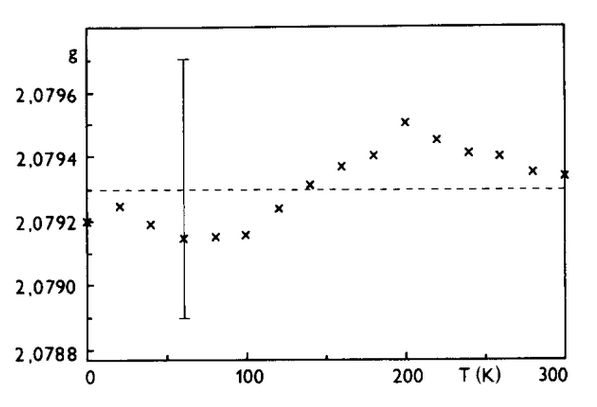
\includegraphics[width=0.8\textwidth]{Frait1981.png}
\caption{Plot of $g$-values vs. temperature taken from \cite{Pust1981}. The vertical bar denotes the accuracy of these values ($\pm0.0004$). }
\label{fig:Frait1981}
\end{figure}

\subsubsection{Magnetic field dependence of $g^{\prime}$}
In the 1950's while Scott was performing precise measurements of $g^{\prime}$, he noticed that $g^{\prime}$ decreased at very low fields and asymptotically approached a larger constant value at higher fields. He published two papers documenting the low-field behavior of $g^{\prime}$ for nickel and iron\cite{ScottAug1955, ScottSep1955}. He concluded that the low-field limit for nickel was $g^{\prime}=1.873\pm0.005$ and its asymptotic value was $g^{\prime}=1.919\pm0.005$ at higher fields. Incidentally, 1.919 is the same value he later more accurately measured as the value for iron. For nickel he determined the low-field limit to be $g^{\prime}=1.801\pm0.002$ and the asymptotic value for higher fields to be $g^{\prime}=1.830$ with no error estimate provided. He later determined the asymptotic value for nickel to be $g^{\prime}=1.835\pm0.002$. 

Scott apparently considered the asymptotic value to be the true value for all fields higher than the low-field region. He did not specifically give information on the strength of the magnetic field used in his higher field measurements, but piecing together information from his papers, it would appear that measurements were all made in the fews tens of Gaus\footnote{To estimate the applied magnetic field in Scott's experiments I assumed from the drawing in figure 4 of \cite{Scott1962} that the magnetic coil was about the same size as the nickel and iron cylindrical samples which were 22~cm long and 1.5~cm in diameter. The ``winding constant'' of the coil was about 78,500~cm$^2$, which I divided by the cross-sectional area and the length to get the number of turns per meter n$\approx$2000. The maximum current through the coil appears to be 16~mA which makes the applied field $H=\mu_0nI\approx 4$~mT=40~G.}. It is natural to wonder if this value truly is asymptotic or if it changes at high field. 

We can again gain insight from FMR measurements of spectroscopic $g$. FMR measurements are made by sweeping the uniform magnetic field strength typically through ranges of order 1~T (see for example Fig. 3 and Table 1 of \cite{Bloembergen1950} where the nickel sample is saturated). As noted in Eq. \ref{eq:fmr}, the resonant frequency depends on the magnetization of the sample. Thus, in order to find the $g$-factor, one has to know {\it a priori} the magnetization of the sample. For ferromagnetic elements, the saturation magnetization is well-determined from the literature and is repeatable i.e. there is a single saturation magnetization value for a given field and temperature. Therefore, these measurements are taken with a saturated sample. We can this consider these to be high-field measurements of the $g$-factor. Furthermore, many FMR measurements take data at multiple frequencies requiring a range of magnetic fields for the different resonance frequencies.

In 1971, Z. Frait and R. Gemperle measured the $g$-factor of single iron crystals across a range of frequencies from 12 to 70~GHz requiring a broad range of static magnetic fields which I estimate to be from 0.1~T to higher than 1.5~T. They found that $g=2.089\pm0.007$ and that it  is frequency independent over this range within their experimental error, constituting a $\sim$0.3\% test of the field dependence of $g$\cite{Frait1971}. In 1977, Z. Frait published an FMR measurement of $g=2.088\pm0.008$ for pure polycrystalline iron at three frequencies, 26~GHz (at 0.32~T), 36~GHz (at 0.57~T) and 70~GHz (at 1.53~T)\cite{Frait1977}. Once again he concluded that within experimental error this value is frequency independent. This constitutes a 0.4\% high-field test of field dependence on $g$ on iron. Taken together these constitute a 0.25\% test of the field dependence of $g$ on iron. In addition, the 0.024\% measurement of the $g$-factor of Fe-3wt\%Si by Pust {\it et al.} was accomplished by averaging measurements at four different frequencies, 36~GHz, 70~GHz, 86~GHz and 95~GHz\cite{Pust1981}. Information in a later paper shows that their electromagnet was capable of creating fields as high as 3~T which sets the scale of the range of these measurements\cite{Pust1984}. They averaged their measurements taken at the four different frequencies (and by extension magnetic fields) to obtain the final result. Although no specific statement is made about the frequency independence of these measurements, the fact that the values were averaged and a tiny error assigned seems to point to a small or non-existent systematic frequency dependence. Finally, we can connect these observations of the field-independence of $g$ with $g^{\prime}$ using Eq. \ref{eq:kittelvanvleck}. I conclude that within the error of the experimental data available $g$ and $g^{\prime}$ appear to be field-independent at least in fields high enough to saturate the sample. Furthermore, the value of $g^{\prime}$ for iron derived from high-field measurements of $g$ agrees well with the low field direct measurements of $g^{\prime}$ consistent with the determination of Scott that $g^{\prime}$ asymptotically approaches the low-field value he measured.

For nickel the data are less precise but point to the same conclusion that $g$ is field-independent. In 1950 Bloembergen measured the $g$-factor of nickel to be 2.23 at 9.05~GHz with a field of 0.116~T and 2.24 at 22.44~GHz with a magnetic field of 0.54~T. These values are equal within the error of the experiment. In 1959, Rodbell found that for nickel $g$ was constant at the 0.5\% level over a range of magnetic fields up to 0.3~T\cite{Rodbell1959}. In 1965, Frait found that $g$ was independent of frequency for pure nickel at the 2\% level over a range of frequencies from 8.5~GHz to 72~GHz. He also found that an alloy consisting of 42\% Fe and 58\% Ni was independent of frequency over the same range at the 1\% level. I estimate the fields for this range to be as high as 1.5~T. Finally, as we saw earlier in Section \ref{sec:gp_temp_dep} the value of $g^{\prime}$ for nickel derived from high-field measurements of $g$ agrees well within error with the direct measurements at low field, providing further evidence of the validity of the asymptotic value of $g^{\prime}$ for nickel.  

For pure iron I would argue from the agreement of $g^{\prime}$ derived from Eq. \ref{eq:kittelvanvleck} that there is no evidence of $g^{\prime}$ depending on magnetic field at the 0.25\% level. Combining this with what appears to be the lack of frequency dependence in Fe-3wt\%Si for extremely accurate measurements gives me confidence that the asymptotic direct measurements of $g^{\prime}$ for iron measured at comparatively low fields are valid. For nickel the value of $g$ is not known as accurately so the comparison between $g^{\prime}$ derived from high-field values of $g$ and the low field measurements of $g^{\prime}$ suffer from $\sim$0.5\% level uncertainties. Within this level of uncertainty $g^{\prime}$ does not appear to depend on magnetic field.  Without evidence to the contrary I would recommend taking the direct low-field asymptotic measurements of $g^{\prime}$ and including no additional uncertainty for magnetic field dependence. 

\FloatBarrier
\section{Calculation of Target Polarization}\label{sec:final_calc}
We are now in a position to calculate the final target polarization and the uncertainty on the value. Tables \ref{tab:final_errors_Fe} and \ref{tab:final_errors_Ni} provide the path to final target polarization from the measured values of saturation magnetization and $g^{\prime}$ for Fe and Ni respectively. The values for magnetization and polarization are calculated for applied magnetic fields of 4~T and 2~T for Fe and Ni foils respectively. In the calculation of target polarization by deBever {\it et al.} in \cite{deBever1997} an equivalence is drawn between target electron polarization and the average electron magnetic moment. This is an approximation valid in the limit that $g_{sp}=2$ and introduces an error at the 0.1\% level. The calculation is as follows:
\[
\hat{\mu}=g_{sp}\frac{e}{2m_e}\hat{S_z}=g_{sp}\mu_B\frac{1}{\hbar}\hat{S_z}.
\]
Substituting the eigenvalues of spin $S_z=\pm\hbar/2$ gives
\[
\mu=\pm\frac{g_{sp}}{2}\mu_B.
\]
Thus the spin of an electron is approximately 1.00116$\mu_B$.

Temperature corrections due to target heating are calculated for a 1~$\mu$A beam load. To first order increasing the beam load linearly increases the temperature correction whereas increasing target thickness leaves the temperature unchanged. Therefore, increasing foil thickness is the better choice for higher scattering rates. 
\begin{table}[h]
\begin{center}
\begin{tabular}{|l|l|l|c|}\hline
Quantity&Value&Error&Unit\\\hline
Saturation Magnetization $M_s$&217.95&0.33&emu/g\\
Saturation Magnetization $M_s$&2.1793&0.0033&$\mu_B/$atom\\
$g^{\prime}$&1.920&0.004&$-$\\
$\frac{M_{orb}}{M_{tot}}=\frac{g_{sp}-g^{\prime}}{g^{\prime}(g_{sp}-1)}$&0.0428&0.0022&$-$\\
Magnetization from orbital motion $M_{orb}$&0.0932&0.0048&$\mu_B$\\
Magnetization from spin $(M_s-M_{orb})$&2.0861&0.0058&$\mu_B$\\
Average electron magnetization (T=294 K, B=4~T)&0.08023&0.00022&$\mu_B/$atom\\
Average electron magnetization (T=313 K, B=4~T)&0.08008&0.00024&$\mu_B/$atom\\
Average electron polarization (T=294 K, B=4~T)&0.08014&0.00022&$-$\\
Average electron polarization (T=313 K, B=4~T)&0.07999&0.00024&$-$\\\hline
\end{tabular}
\end{center}
\caption{\label{tab:final_errors_Fe}Summary of values and errors involved in calculating the target polarization for Fe foils. The ratio of electron magnetization in Bohr magnetons and electron polarization is $g_{sp}/2\approx1.0012$ not unity as supposed in \cite{deBever1997}.}
\end{table}

\begin{table}[h]
\begin{center}
\begin{tabular}{|l|l|l|c|}\hline
Quantity&Value&Error&Unit\\\hline
Saturation Magnetization $M_s$&55.20&0.14&emu/g\\
Saturation Magnetization $M_s$&0.5801&0.0015&$\mu_B/$atom\\
$g^{\prime}$&1.841&0.005&$-$\\
$\frac{M_{orb}}{M_{tot}}=\frac{g_{sp}-g^{\prime}}{g^{\prime}(g_{sp}-1)}$&0.0874&0.0030&$-$\\
Magnetization from orbital motion $M_{orb}$&0.0507&0.0018&$\mu_B/$atom\\
Magnetization from spin $(M_s-M_{orb})$&0.5294&0.0023&$\mu_B/$atom\\
Average electron magnetization (T=294 K, B=2~T)&0.018907&0.000084&$\mu_B$\\
Average electron magnetization (T=313 K, B=2~T)&0.018732&0.000089&$\mu_B$\\
Average electron polarization (T=294 K, B=2~T)&0.018885&0.000084&$-$\\
Average electron polarization (T=313 K, B=2~T)&0.018710&0.000089&$-$\\\hline
\end{tabular}
\end{center}
\caption{\label{tab:final_errors_Ni}Summary of values and errors involved in calculating the target polarization for Ni foils.}
\end{table}

It is important to verify at the $<$0.1\% level that the target indeed is saturated at the final magnetic field settings. Diagrams such as Figs. 1 and 2 in \cite{deBever1997} imply that a perfectly aligned foil will saturate out-of-plane at 2.2~T, which is the saturation magnetization of Fe and that if it does not thenalignment is the most likely issue. However, numerous other effects such as ``impurities, strains, anisoptropic contributions, geometric effects etc.'' prevent saturation \cite{Foner1969}. Foner {\it et al.} found for an Fe foil that ``although the saturation value of $H_{DM}$\footnote{$H_{DM}$ is the demagnetizing field which for the case of a thin iron foil magnetized out of plane is $4\pi M=21.8~\textrm{kG}=2.18$~T.} is 21.8~kG, because of the anisotropy energy associated with the rotation of domains and the movement of domains boundaries, we have experimentally determined that fields of the order of 30~kG applied perpendicular to the plane of the iron foil are necessary to align completely the magnetization along the external field direction''\cite{Foner1969}.   
 

\section{Concluding Discussion}\label{conclusions}
The polarization of a saturated ferromagnetic target has been calculated for both nickel and iron foils. With the stringent demands of the proposed MOLLER experiment, it seemed wise to revisit the claim that the polarization of an Fe target was known to 0.2\% as claimed by deBever {\it et al.}\cite{deBever1997}. A different approach was taken than that in \cite{deBever1997} where instead of using the saturation magnetization value at 0~K and then correcting back to room temperature, measured values of magnetization were taken at or near room temperature. A small error was found in the magnetic field correction in equation (3) of \cite{deBever1997} where the applied magnetic field was used instead of the internal magnetic field, introducing a small error of about 0.1\%. A couple of approximations also introduced further errors of order 0.1\% in \cite{deBever1997}. These were as follows: 

1). The expression $M_{orb}/M_{tot}=(2-g^{\prime})/g^{\prime}$ used to calculate the orbital and spin components of the magnetization is an approximate expression which more accurately is given by Eq.~\ref{eq:gprime_exact}. 

2). The equating of electron target polarization and average electron magnetization in units of $\mu_B$ is true only in the approximation $g^{\prime}/2=1$. 

The error in target polarization listed in the MEI proposal for the MOLLER experiment was 0.25\%. This study concludes that the polarization at room temperature of a saturated Fe foil can be known to 0.28\% and that of an Ni foil to 0.45\%.  Additional uncertainty associated with the temperature correction under a 1~$\mu$A electron beam load takes the relative uncertainties for Fe and Ni to 0.3\% and 0.48\%.  However, the combination of measurements on Ni and Fe foils will reach the 0.25\% level even under a 1~$\mu$A beam load.

\FloatBarrier
%% The Appendices part is started with the command \appendix;
%% appendix sections are then done as normal sections
%% \appendix

%% \section{}
%% \label{}

%% If you have bibdatabase file and want bibtex to generate the
%% bibitems, please use
\bibliographystyle{elsarticle-num} 
%%  \bibliography{<your bibdatabase>}

%% else use the following coding to input the bibitems directly in the
%% TeX file.

\bibliography{bibliography}
\end{document}
%\endinput
%%
%% End of file `elsarticle-template-num.tex'.
� 2020 GitHub, Inc.
Terms
Privacy
Security
Status
Help
Contact GitHub
Pricing
API
Training
Blog
About
